% ============================================================================
% Thermodynamic Dynamics of\\Observer-Memory Entanglement
% Complete Collected Volume
% ============================================================================

\documentclass[12pt,a4paper,openany]{book}

\usepackage[utf8]{inputenc}
\usepackage[T1]{fontenc}
\usepackage{amsmath,amssymb,amsfonts,amsthm}
\usepackage{mathtools}
\usepackage{mathrsfs}
\usepackage{physics}
\usepackage{graphicx}
\usepackage[hidelinks]{hyperref}
\usepackage{tikz}
\usetikzlibrary{shapes,arrows,positioning,calc,decorations.pathmorphing}
\usepackage{geometry}
\usepackage{fancyhdr}
\usepackage{titlesec}
\usepackage{array}
\newcolumntype{P}[1]{>{\raggedright\arraybackslash}p{#1}}
\usepackage{booktabs}
\usepackage{tcolorbox}
\usepackage{xcolor}
\usepackage{caption}
\usepackage{float}
\usepackage{enumitem}
\usepackage{newunicodechar}
\newunicodechar{आ}{\textit{aa}}
\newunicodechar{ल}{\textit{la}}
\newunicodechar{य}{\textit{ya}}
\newunicodechar{व}{\textit{va}}
\newunicodechar{ि}{\textit{i}}
\newunicodechar{ज}{\textit{ja}}
\newunicodechar{ञ}{\textit{~na}}
\newunicodechar{न}{\textit{na}}
\newunicodechar{श}{\textit{sha}}
\newunicodechar{ू}{\textit{uu}}
\newunicodechar{ण}{\textit{.na}}
\newunicodechar{त}{\textit{ta}}
\newunicodechar{ा}{\textit{aa}}
\newunicodechar{स}{\textit{sa}}
\newunicodechar{भ}{\textit{bha}}
\newunicodechar{ृ}{\textit{.r}}
\newunicodechar{ह}{\textit{ha}}
\newunicodechar{्}{}
\newunicodechar{§}{\S{}}
\newunicodechar{É}{\'{E}}
\newunicodechar{ñ}{\~{n}}
\newunicodechar{Ā}{\={A}}
\newunicodechar{ā}{\={a}}
\newunicodechar{ś}{\'{s}}
\newunicodechar{ū}{\={u}}
\newunicodechar{ṃ}{\d{m}}
\newunicodechar{ṅ}{\.{n}}
\newunicodechar{ṇ}{\d{n}}
\newunicodechar{—}{---}

\graphicspath{{TDOME_Complete_supplement/}{TDOME_I_supplement/}{TDOME_II_supplement/}{TDOME_III_supplement/}}
\geometry{a4paper, margin=1in, headheight=28pt}

\newtheorem{theorem}{Theorem}[chapter]
\newtheorem{proposition}[theorem]{Proposition}
\newtheorem{lemma}[theorem]{Lemma}
\newtheorem{definition}[theorem]{Definition}
\newtheorem{remark}[theorem]{Remark}
\newtheorem{corollary}[theorem]{Corollary}
\newtheorem{conjecture}[theorem]{Conjecture}
\newtheorem{constraint}[theorem]{Constraint}
\newtheorem{example}[theorem]{Example}
\newtheorem{assumption}[theorem]{Assumption}
\newtheorem{criterion}[theorem]{Criterion}


\pagestyle{fancy}
\fancyhf{}
\fancyhead[LE,RO]{\thepage}
\fancyhead[RE]{\textit{Thermodynamic Dynamics of Observer-Memory Entanglement}}
\fancyhead[LO]{\textit{\leftmark}}
\renewcommand{\headrulewidth}{0.4pt}

\title{
  \vspace{-2cm}
  {\Huge\textbf{Thermodynamic Dynamics of\\Observer-Memory Entanglement}}\\[1cm]
  {\Large\textit{Memory, Ego, and Self-Referential Calibration\\ in Persistent Far-from-Equilibrium Systems}}\\[2cm]
  {\large Complete Collected Volume}\\[0.5cm]
  {\normalsize Papers I, II, and III}
}

\author{
  \textbf{Sidong Liu, PhD}\\[0.5em]
  iBioStratix Ltd\\[0.3em]
  \texttt{sidongliu@hotmail.com}
}

\date{July 2026}

\begin{document}
\emergencystretch=2em
\raggedbottom
\hbadness=10000
\vbadness=10000

\frontmatter
\maketitle

\newpage
\thispagestyle{empty}
\vspace*{\fill}
\begin{center}
\textbf{Publication Record}\\[2em]
\begin{tabular}{ll}
Paper I & DOI: 10.5281/zenodo.18574342 \\
Paper II & DOI: 10.5281/zenodo.18579703 \\
Paper III & DOI: 10.5281/zenodo.18591771 \\
\end{tabular}
\\[3em]
\textit{This collected volume compiles previously published works\\
for archival and reference purposes.}
\\[2em]
\copyright{} 2026 Sidong Liu. All rights reserved.
\end{center}
\vspace*{\fill}

\chapter*{Abstract}
\addcontentsline{toc}{chapter}{Abstract}

This volume develops conditional models of persistent agency under thermodynamic, computational, and calibration constraints.

The three papers are not presented as an irreversible proof of necessary observer architecture.  Paper I gives a restricted Markovian baseline and a conditional memory advantage when usable system--environment correlations are supplied.  Paper II studies a declared archive and coordinate-projection model in which compression can reduce computational load.  Paper III analyzes a specified self-referential calibration implementation and its costs under explicit likelihood, drift, convexity, and hardware assumptions.

Together, the papers define a running architecture of memory, reference-frame selection, and second-order calibration.  The architecture is a model template and test bed, not a proof that all persistent agents require these layers or that the list is necessary, sufficient, minimal, or complete.

\bigskip
\noindent\textbf{Keywords}: non-Markovian dynamics, open quantum systems, memory kernel, reference-frame selection, bounded rationality, Fisher information, information geometry, self-referential calibration, Lyapunov stability, implementation cost

\tableofcontents

\mainmatter

% ============================================================================
% Paper I --- ``The Seed''
% ============================================================================
\chapter{Non-Markovian Memory and Temporal Accumulation: A Conditional Thermodynamic Analysis}
\label{chap:paperI}

\begin{center}
\textit{Paper I --- ``The Seed''}\\[0.5em]
Originally published: Zenodo, DOI: 10.5281/zenodo.18574342
\end{center}

\bigskip

\section*{Abstract}
We investigate a conditional thermodynamic role for memory in open
quantum systems interacting with stochastic environments.  Working
within stochastic and information thermodynamics, we define a
\emph{survival functional} $\mathcal{S}:=\Delta F-W$ measuring the
difference between non-equilibrium free energy gained and work invested
by an agent.

For a fixed-Hamiltonian autonomous Davies/GKSL baseline with no
measurement or feedback, we prove a restricted Markovian ceiling:
$\mathcal{S}\leq0$.  This is not a universal ceiling for driven or
feedback-controlled Markovian agents.  We then derive an accounting
identity for finite-dimensional autonomous evolution, with the
interaction-energy term retained or a declared weak-coupling
approximation made, expressing the survival functional through changes
in system--environment mutual information and bath displacement.  In
models where prior interaction has supplied usable correlations, their
consumption during non-Markovian backflow intervals can yield
$\mathcal{S}>0$, bounded by the initial correlation budget.

The result is therefore a conditional memory advantage, not a proof that
memory or non-Markovianity is necessary or sufficient for all persistent
systems.  Fisher accretion and the comparison with the accessibility
ordering of the Holographic Alaya-Field Framework (HAFF) are presented
as heuristics.  A worked spin-boson example with Lorentz--Drude spectral
density illustrates how the accounting can operate in one supplied
model.

Finally, using entropy rate and predictive information from
computational mechanics, we study the implementation cost of a specified
irreversible archive-reset model.  Universal Landauer costs for merely
storing or maintaining memory, and the resulting universal ``Memory
Catastrophe,'' are withdrawn; only the declared archive implementation
is charged.

\medskip
\noindent\textbf{Keywords}: non-Markovian dynamics, open quantum systems,
Nakajima--Zwanzig equation, memory kernel, thermodynamic arrow of time,
information backflow, entropy production, stochastic thermodynamics


% ============================================================
\section{Introduction}
\label{I-sec:intro}

% ------------------------------------------------------------
\subsection{Context: The Problem of Persistence}

A quantum system coupled to a thermal environment generically
relaxes toward equilibrium. This is the content of the
\emph{zeroth crisis}: absent special structure, every open
subsystem is eventually erased by thermal noise~\cite{BreuerPetruccione2002}.

Yet the physical world contains persistent far-from-equilibrium
structures---from molecular machines to living organisms---that
maintain themselves against the entropic tide for timescales
vastly exceeding their intrinsic relaxation times. What
structural feature of their dynamics makes this possible?

The standard answer invokes free-energy input: a persistent system
continuously imports low-entropy energy and exports high-entropy
waste~\cite{Schrodinger1944}.  This paper asks the narrower accounting
question of when pre-existing system--environment correlations can fund
a later interval.  It does not claim that memory distinguishes every
persistent system from every non-persistent one.

% ------------------------------------------------------------
\subsection{Position within the Series}

This paper is the first of three constituting the
\textbf{T-DOME} (Thermodynamic Dynamics of Observer-Memory
Entanglement) framework, the third pillar of a three-paper
program.

\begin{center}
\small
\setlength{\tabcolsep}{4pt}%
\begin{tabular}{@{}lP{3.2cm}cP{3.4cm}c@{}}
\toprule
\textbf{Framework} & \textbf{Question} & & \textbf{Result} & \textbf{Status} \\
\midrule
HAFF~\cite{Liu2026HAFF_A,Liu2026HAFF_B}
  & How does geometry emerge?
  & Ocean
  & Conditional algebra/dictionary models
  & Revised \\[3pt]
Q-RAIF~\cite{Liu2026QRAIF_A,Liu2026QRAIF_B}
  & What algebra must an observer have?
  & Fish
  & Clifford representation as model input
  & Revised \\[3pt]
\textbf{T-DOME I} (this work)
  & What can inter-epoch correlations fund?
  & Seed
  & ELV-type accounting identity; restricted ceiling
  & \textbf{This paper} \\[3pt]
T-DOME II
  & How can a supplied archive be budgeted?
  & Ego
  & Conditional feature selection
  & Companion \\[3pt]
T-DOME III
  & When can residual statistics track drift?
  & Loop
  & Conditional Fisher calibration
  & Companion \\
\bottomrule
\end{tabular}
\end{center}

The three T-DOME papers form a conditional modelling sequence,
not an irreversible theorem chain:
\begin{enumerate}
\item \textbf{Paper I (The Seed):} The accounting identity asks when
  correlations built in earlier epochs can fund a later interval.
  A deliberately uncompressed archive is then introduced only as
  motivation for a finite-budget problem.
\item \textbf{Paper II (The Ego):} Given that archive model and a
  supplied component representation, Paper II studies conditional
  feature selection under a processing budget.
\item \textbf{Paper III (The Loop):} Given a selected frame and an
  explicit residual likelihood, Paper III studies conditions under
  which a calibration controller can track drift.
\end{enumerate}

\noindent
The present paper addresses only the first link in this chain.

% ------------------------------------------------------------
\subsection{Relation to HAFF Paper F}

Revised HAFF Paper F~\cite{Liu2026HAFF_F} treats record growth and
algebra inclusion as protocol-relative orderings and does not derive
a universal temporal partial order.  Section~\ref{I-sec:arrow} therefore
uses it only as motivation: a memory-influence relation and a
pointer-record ordering may be compared after both are supplied, but
neither is proved to embed in the other.

% ------------------------------------------------------------
\subsection{Scope and Disclaimers}

\begin{enumerate}
\item This work does \emph{not} claim that memory or
  non-Markovianity is necessary for persistence.  Continuously driven
  Markovian dissipative structures can persist.  The narrower claim is
  that pre-existing inter-epoch correlations can fund a positive
  interval of the survival accounting functional.
\item The sign of that functional is governed by changes in initial
  correlation and bath-displacement resources, not by Markovianity as
  such.  No strict comparison of Markovian and non-Markovian suprema is
  proved.
\item We do \emph{not} derive the specific form of the memory
  kernel from first principles. The kernel is treated as a
  structural feature of the system-environment coupling.
\item The term ``agent'' is used in the control-theoretic sense
  (a subsystem that acts on its environment to maintain a target
  state) and carries no implication of consciousness, intention,
  or subjective experience.
\item A broader structural analogy with classical philosophical
  concepts of temporal persistence exists but is outside the
  scope of this paper.
\end{enumerate}

\paragraph{Result-status ledger.}
The information--thermodynamic identity is a general finite-dimensional
unitary accounting identity (GvN/THM/OK-cond, with the interaction-energy
term retained or a declared weak-coupling approximation).  The original
time-dependent-control Markovian Ceiling is retracted; a narrower
autonomous Davies-semigroup theorem is proved below (FD/I/THM/OK-cond).
Fisher accretion and the HAFF bridge are heuristics.  Universal
Landauer costs for storing or maintaining memory and the resulting
``Memory Catastrophe'' are retracted; only a specified irreversible
archive-reset model remains.

% ============================================================
\section{Mathematical Preliminaries}
\label{I-sec:prelim}

% ------------------------------------------------------------
\subsection{Open Quantum Systems: The Markovian Baseline}

Consider a bipartite Hilbert space
$\mathcal{H} = \mathcal{H}_R \otimes \mathcal{H}_E$,
where $R$ denotes the ``agent'' (reduced system) and $E$ the
environment. The total Hamiltonian is
\begin{equation}
\label{I-eq:H_total}
H = H_R \otimes \mathbb{1}_E
  + \mathbb{1}_R \otimes H_E
  + \lambda\, H_{\mathrm{int}},
\end{equation}
where $\lambda$ parametrizes the coupling strength.

Under the Born--Markov and secular approximations, the reduced
dynamics of $\rho_R(t) = \mathrm{Tr}_E[\rho(t)]$ is governed by
the Gorini--Kossakowski--Sudarshan--Lindblad (GKSL) master
equation~\cite{Lindblad1976,GKS1976}:
\begin{equation}
\label{I-eq:GKSL}
\dot{\rho}_R(t)
= -i[H_{\mathrm{eff}},\, \rho_R(t)]
  + \sum_k \gamma_k \left(
    L_k \rho_R(t) L_k^\dagger
    - \tfrac{1}{2}\{L_k^\dagger L_k,\, \rho_R(t)\}
  \right),
\end{equation}
with $\gamma_k \geq 0$ and Lindblad operators $\{L_k\}$.

\begin{remark}[Markovian = Memoryless]
\label{I-rem:markov}
The GKSL equation is \emph{time-local}: $\dot{\rho}_R(t)$ depends
only on $\rho_R(t)$, never on $\rho_R(s)$ for $s < t$.
Physically, this corresponds to an environment with vanishing
correlation time ($\tau_E \to 0$): the bath ``forgets'' its
interaction with the system instantaneously.
The semigroup property $\Lambda(t+s) = \Lambda(t)\Lambda(s)$
ensures complete positivity at all times but precludes any
information backflow from environment to system~\cite{RivasHuelgaPlenio2014}.
\end{remark}

% ------------------------------------------------------------
\subsection{Beyond Markov: The Nakajima--Zwanzig Equation}

When the environmental correlation time $\tau_E$ is non-negligible,
the Born--Markov approximation fails. The exact reduced dynamics
is captured by the Nakajima--Zwanzig (NZ) integro-differential
equation~\cite{Nakajima1958,Zwanzig1960}:
\begin{equation}
\label{I-eq:NZ}
\dot{\rho}_R(t)
= -i[H_{\mathrm{eff}},\, \rho_R(t)]
  + \int_0^t ds\; \mathcal{K}(t,s)\, \rho_R(s),
\end{equation}
where $\mathcal{K}(t,s)$ is the \textbf{memory kernel}---a
superoperator encoding the influence of the system's entire
history on its present dynamics.

\begin{definition}[Memory Kernel]
\label{I-def:kernel}
The memory kernel $\mathcal{K}: [0,\infty)^2 \to
\mathcal{L}(\mathcal{B}(\mathcal{H}_R))$ is the superoperator
satisfying~\eqref{I-eq:NZ}. It encodes two types of information:
\begin{enumerate}
\item \textbf{Environmental structure:} the spectral density,
  correlation functions, and non-equilibrium features of the bath;
\item \textbf{Temporal reach:} the effective support
  $\tau_{\mathrm{mem}} := \inf\{\tau : \|\mathcal{K}(t,s)\| < \epsilon
  \;\forall\; t - s > \tau\}$, the ``memory depth.''
\end{enumerate}
The Markovian limit corresponds to
$\mathcal{K}(t,s) \to \mathcal{K}_0\, \delta(t-s)$,
recovering the GKSL generator.
\end{definition}

\begin{remark}[Information Backflow]
\label{I-rem:backflow}
Non-Markovian dynamics admits \emph{information backflow}:
the distinguishability of two initial states, as measured by
trace distance $D(\rho_1(t), \rho_2(t))$, can temporarily
increase~\cite{BreuerLainePiilo2009}. This is the operational
signature of memory---the environment returns previously
absorbed information to the system.
\end{remark}

% ------------------------------------------------------------
\subsection{Thermodynamic Framework}
\label{I-subsec:thermo}

We adopt the framework of stochastic thermodynamics for open
quantum systems~\cite{EspositoLindenbergVandenBroeck2010}.
The following conventions are fixed throughout.

\begin{definition}[Thermodynamic Setup]
\label{I-def:thermo_setup}
\leavevmode
\begin{enumerate}
\item \textbf{Hamiltonian decomposition.}
  The system Hamiltonian is
  $H_S(t) = H_R + H_{\mathrm{ctrl}}(t)$,
  where $H_R$ is the \emph{fixed} bare Hamiltonian and
  $H_{\mathrm{ctrl}}(t)$ is the agent's time-dependent
  control protocol.
  The bath Hamiltonian $H_E$ and coupling $H_{\mathrm{int}}$
  are as in~\eqref{I-eq:H_total}.

\item \textbf{Reference state.}
  The thermal equilibrium state of the bare Hamiltonian is
  \begin{equation}
  \label{I-eq:rho_eq}
  \rho_{\mathrm{eq}} := \frac{e^{-\beta H_R}}{Z_R},
  \qquad Z_R := \tr(e^{-\beta H_R}),
  \qquad \beta := (k_B T)^{-1}.
  \end{equation}
  Since $H_R$ is time-independent, $\rho_{\mathrm{eq}}$ is a
  well-defined, fixed reference throughout the protocol.

\item \textbf{Non-equilibrium free energy.}
  For any state $\rho$ of the reduced system,
  \begin{equation}
  \label{I-eq:F_neq}
  F(\rho) := \tr(\rho\, H_R) + \beta^{-1}\tr(\rho\ln\rho)
  = \langle H_R \rangle_\rho - \beta^{-1} S(\rho),
  \end{equation}
  where $S(\rho) = -\tr(\rho\ln\rho)$ is the von~Neumann entropy.
  The equilibrium value is $F_{\mathrm{eq}} = -\beta^{-1}\ln Z_R$.

\item \textbf{Free energy--relative entropy identity.}
  \begin{equation}
  \label{I-eq:DKL_F}
  D_{\mathrm{KL}}(\rho \| \rho_{\mathrm{eq}})
  = \beta\bigl(F(\rho) - F_{\mathrm{eq}}\bigr) \geq 0.
  \end{equation}
  Thus $D_{\mathrm{KL}}$ measures the free-energy surplus in
  units of $k_B T$.

\item \textbf{Work.}
  The inclusive work performed on the total system by the control protocol
  over $[0,\tau]$ is
  \begin{equation}
  \label{I-eq:work}
  W[0,\tau] := \int_0^\tau
  \tr\!\left(\rho(t)\,
  \frac{\partial H_{\mathrm{ctrl}}}{\partial t}\right) dt.
  \end{equation}

\item \textbf{Entropy-production functional.}
  The \emph{generalised entropy production} over $[0,\tau]$ is
  \begin{equation}
  \label{I-eq:Sigma}
  \Sigma[0,\tau] := \beta\bigl(W[0,\tau] - \Delta F\bigr),
  \end{equation}
  where $\Delta F = F(\rho(\tau)) - F(\rho(0))$.
  For uncorrelated (product) initial states,
  $\Sigma \geq 0$ recovers the standard second-law bound.
  For initially correlated states, $\Sigma$ can be
  \emph{negative}, reflecting the consumption of
  pre-existing correlations
  (see Remark~\ref{I-rem:battery}).
\end{enumerate}
\end{definition}

\begin{remark}[Why $H_R$ is fixed]
\label{I-rem:H_fixed}
The bare Hamiltonian $H_R$ defines the system's energy scale and
hence the reference state $\rho_{\mathrm{eq}}$.
The agent acts on the world through $H_{\mathrm{ctrl}}(t)$,
which may be time-dependent.
This separation ensures that $\rho_{\mathrm{eq}}$ is
well-defined and time-independent for the accounting identity.
It does \emph{not} make a driven generator satisfy detailed balance
with respect to that fixed state.  The ceiling result below therefore
uses autonomous $H_{\mathrm{ctrl}}=0$ dynamics.
\end{remark}

\begin{definition}[Standing Assumptions]
\label{I-def:assumptions}
The following minimal assumptions are in force throughout
Sections~\ref{I-sec:advantage}--\ref{I-sec:example} unless
stated otherwise.
Every main result
(Lemma~\ref{I-lem:info_thermo},
Theorem~\ref{I-thm:advantage},
Corollary~\ref{I-cor:three_regimes})
relies \emph{only} on items
\textup{(A1)--(A5)} below.
\begin{enumerate}
\item[\textup{(A1)}]
  \textbf{Finite-dimensional bipartite system.}
  $\mathcal{H} = \mathcal{H}_S \otimes \mathcal{H}_E$,
  with total Hamiltonian~\eqref{I-eq:H_total}
  and global unitary evolution
  $U(t) = \mathcal{T}\exp(-i\int_0^t H(s)\,ds)$.

\item[\textup{(A2)}]
  \textbf{Weak coupling.}
  The system--environment interaction satisfies
  $\lambda \ll 1$ in~\eqref{I-eq:H_total}, so that
  $\Delta\langle H_{\mathrm{int}} \rangle
  = O(\lambda)$~\cite{BreuerPetruccione2002}.
  The first-law bookkeeping is
  $W=\Delta\langle H_R\rangle
  + \Delta\langle H_{\mathrm{ctrl}}\rangle
  + \Delta\langle H_E\rangle
  + \Delta\langle H_{\mathrm{int}}\rangle$.
  Dropping the last term is the declared weak-coupling approximation
  $\Delta\langle H_{\mathrm{int}}\rangle=O(\lambda)$; it is not
  an energy-conservation equation with a zero right-hand side.

\item[\textup{(A3)}]
  \textbf{Fixed environmental reference.}
  $\rho_E^{\mathrm{th}} := e^{-\beta H_E}/Z_E$
  is a fixed \emph{bookkeeping} Gibbs state at inverse
  temperature $\beta$.
  The \emph{actual} initial bath state $\rho_E(0)$
  need not coincide with $\rho_E^{\mathrm{th}}$;
  when $\rho_E(0) \neq \rho_E^{\mathrm{th}}$, the quantity
  $D_{\mathrm{KL}}(\rho_E(t)\|\rho_E^{\mathrm{th}})$
  tracks the nonequilibrium free energy stored in the bath
  relative to this reference.
  The bath Hamiltonian $H_E$ is time-independent.

\item[\textup{(A4)}]
  \textbf{Arbitrary initial state.}
  The total initial state $\rho_{SE}(0)$ is \emph{not}
  required to be a product state.
  In particular, initial system--environment correlations
  $I(S{:}E;\,0) > 0$ and initial bath displacement
  $D_{\mathrm{KL}}(\rho_E(0)\|\rho_E^{\mathrm{th}}) > 0$
  are both permitted.
\item[\textup{(A5)}]
  \textbf{Regularity.}
  All quantum states appearing in the thermodynamic
  identities are assumed to have full rank (or are
  restricted to their support), so that all relative
  entropies $D_{\mathrm{KL}}(\rho\|\sigma)$ are finite.
\end{enumerate}
\end{definition}

\begin{remark}[Bookkeeping conventions]
\label{I-rem:bookkeeping}
The heat absorbed by the environment is
$Q := \Delta\langle H_E \rangle
= \mathrm{Tr}[\rho_E(\tau) H_E]
  - \mathrm{Tr}[\rho_E(0) H_E]$
(matching
Esposito \emph{et al.}~\cite{EspositoLindenbergVandenBroeck2010}).
We define $\Sigma := \beta(W - \Delta F)$ as a
\emph{generalised entropy-balance functional};
for correlated initial conditions $\Sigma$ need not be
nonnegative
(see Remark~\ref{I-rem:battery}).
\end{remark}

% ------------------------------------------------------------
\subsection{The Survival Functional}
\label{I-subsec:survival}

We now define the central quantity of this paper.

\begin{definition}[Survival Functional]
\label{I-def:survival}
For a reduced system $R$ evolving under dynamics $\Lambda$
over $[0,\tau]$, the \textbf{survival functional} is
\begin{equation}
\label{I-eq:survival}
\mathcal{S}[\Lambda, \tau]
:= \Delta F - W[0,\tau]
= \bigl[F(\rho(\tau)) - F(\rho(0))\bigr] - W[0,\tau].
\end{equation}
Equivalently, using~\eqref{I-eq:Sigma},
\begin{equation}
\label{I-eq:survival_Sigma}
\beta\,\mathcal{S}[\Lambda,\tau] = -\Sigma[0,\tau].
\end{equation}
\end{definition}

\noindent\textit{Note on nomenclature.}
We retain the term ``survival functional'' to emphasize
the biological interpretation of persistence far from
equilibrium; mathematically, $\mathcal{S}$ is strictly a
\emph{generalized entropy-balance functional} derived from
the first and second laws.

\begin{remark}[Interpretation]
\label{I-rem:survival_interp}
The survival functional has a transparent physical meaning:
\begin{itemize}
\item $\mathcal{S} > 0$: the system gained more free energy than
  was invested by the external protocol---a \emph{thermodynamic
  profit}. The agent has extracted usable work from environmental
  correlations.
\item $\mathcal{S} = 0$: the agent breaks even (reversible limit,
  $\Sigma = 0$).
\item $\mathcal{S} < 0$: the agent paid more than it gained
  (the generic irreversible case).
\end{itemize}
Under the standard second law ($\Sigma \geq 0$),
$\mathcal{S} \leq 0$ always.
As Section~\ref{I-sec:advantage} shows, a positive interval requires
consumption of a resource present at that interval's initial time,
such as system--environment correlation or bath displacement.
Whether a memory kernel preserves access to that resource is a
model-specific dynamical question.
\end{remark}

\begin{remark}[Connection to Information Thermodynamics]
\label{I-rem:connection_SU}
In the Sagawa--Ueda framework~\cite{SagawaUeda2010,SagawaUeda2012},
a system under feedback control satisfies the generalized second law
\begin{equation}
\label{I-eq:sagawa_ueda}
\Sigma \geq -I_{\mathrm{feedback}},
\end{equation}
where $I_{\mathrm{feedback}} \geq 0$ is the mutual information
gained through measurement of the system.
This permits $\Sigma < 0$ (and hence $\mathcal{S} > 0$) at
the expense of information.
Pre-existing correlations can enter the entropy balance in a role
analogous to measurement information.  A memory kernel is not
automatically a measurement or feedback controller; a concrete model
must show that it preserves and later exposes those correlations.
\end{remark}

% ============================================================
\section{A Restricted Markovian Baseline}
\label{I-sec:ceiling}

The former ``Markovian Ceiling'' allowed a time-dependent control
Hamiltonian while using a fixed bare Gibbs state as the
detailed-balance reference.  A driven generator need not preserve that
state, so the asserted balance law did not follow from Spohn's
inequality.  That theorem, its open-loop control class, and its
temporal-blindness corollary are retracted.  The autonomous result below
is the narrower statement that survives.

\subsection{Spohn's Inequality}

Throughout this section we assume that the GKSL generator
$\mathcal{L}$ is a \emph{thermal Lindbladian}: it is obtained
from the weak-coupling (Davies) limit of a system coupled to a
single thermal bath at inverse temperature $\beta$, and satisfies
\textbf{quantum detailed balance} (the KMS
condition)~\cite{Spohn1978,BreuerPetruccione2002}.
Under this assumption, the unique stationary state is the Gibbs
state $\rho_{\mathrm{ss}} = \rho_{\mathrm{eq}}$
of~\eqref{I-eq:rho_eq}, and the generator is self-adjoint with
respect to the KMS inner product.
This ensures that the entropy production rate below is
well-defined and non-negative.

\begin{definition}[Autonomous Davies baseline]
\label{I-def:autonomous_davies}
The autonomous baseline has $H_{\mathrm{ctrl}}=0$, fixed system
Hamiltonian $H_R$, and a time-independent Davies/GKSL generator
$\mathcal L$ satisfying quantum detailed balance with respect to the
faithful Gibbs state $\rho_{\mathrm{eq}}=e^{-\beta H_R}/Z_R$.
No measurement, feedback, or initial system--bath resource is included
in this reduced semigroup model.
\end{definition}

\begin{lemma}[Spohn~\cite{Spohn1978}]
\label{I-lem:spohn}
For any GKSL dynamical semigroup $\Lambda_t = e^{\mathcal{L}t}$
satisfying quantum detailed balance with unique invariant state
$\rho_{\mathrm{eq}}$, the entropy production
rate
\begin{equation}
\label{I-eq:spohn_sigma}
\sigma(t) := -\tr\!\bigl(\mathcal{L}[\rho(t)]\,
(\ln\rho(t) - \ln\rho_{\mathrm{eq}})\bigr)
\end{equation}
satisfies $\sigma(t) \geq 0$, equivalently
$dD_{\mathrm{KL}}(\rho(t)\|\rho_{\mathrm{eq}})/dt\leq0$.
\end{lemma}

\begin{proof}
This follows from the contractivity of CPTP maps under quantum
relative entropy~\cite{Spohn1978,BreuerPetruccione2002}:
$D_{\mathrm{KL}}(\Lambda_t\rho \| \Lambda_t\rho_{\mathrm{eq}})
\leq D_{\mathrm{KL}}(\rho \| \rho_{\mathrm{eq}})$
for all $t \geq 0$.
Differentiating at $t = 0$ yields $\sigma(t) \geq 0$.
\end{proof}

\subsection{The Restricted Autonomous Ceiling}

\begin{theorem}[Restricted Autonomous Ceiling]
\label{I-thm:autonomous_ceiling}
Under Definition~\ref{I-def:autonomous_davies}, the survival functional
obeys
\begin{equation}
\label{I-eq:ceiling}
\mathcal S[0,\tau]=F(\rho(\tau))-F(\rho(0))\leq0.
\end{equation}
Equality requires no decrease of relative entropy on the interval
(for a primitive semigroup, equilibrium is the stationary equality case).
\end{theorem}

\begin{proof}
Here $W=0$.  By~\eqref{I-eq:DKL_F} and Lemma~\ref{I-lem:spohn},
$\beta\Delta F=\Delta D_{\mathrm{KL}}\leq0$, hence
$\mathcal S=\Delta F\leq0$.
\end{proof}

\begin{remark}[Driven protocols require a different theorem]
\label{I-rem:driven_protocol}
For time-dependent $H_S(t)$ one may define the instantaneous Gibbs
state of the full driven Hamiltonian and assume a generator satisfying
instantaneous detailed balance, together with inclusive work
$\int\tr(\rho\,\dot H_S)dt$.  Those hypotheses describe a different
driven-thermodynamics result and are not proved here.  Open-loop alone
does not repair the missing relation between generator and reference
state; feedback protocols require their own information balance.
\end{remark}

\begin{remark}[Memorylessness and temporal correlations]
\label{I-rem:temporal_blindness}
Under the Born--Markov approximation, the bath correlation
function is replaced by its white-noise limit
$C(t,s) \to C_0\,\delta(t-s)$, and the GKSL dissipator depends
only on the spectral density $J(\omega)$ evaluated at the
system's Bohr frequencies.
The reduced semigroup therefore omits explicit inter-epoch bath
correlations.  This modelling loss does not imply a universal spectral
gap formula, a universal maintenance-work bound, or impossibility of
continuously driven Markovian persistence.
\end{remark}

\begin{remark}[Dissipative vs.\ Self-Nourishing Structures]
\label{I-rem:ceiling_physics}
The restricted theorem is a free-energy monotonicity statement for one
autonomous detailed-balance class.  It does not say that Markovian
systems cannot persist under continuous driving, that non-Markovianity
is necessary for persistence, or that a memory kernel alone supplies
usable feedback.  It is a controlled baseline for comparisons at fixed
initial resources.
\end{remark}

% ============================================================
\section{Initial-Correlation Accounting}
\label{I-sec:advantage}

We now separate a dynamics-agnostic accounting identity from the
model-dependent question of memory.  Quantum mutual information
$I(S{:}E)$ can be a consumable initial resource.  A non-Markovian model
may preserve such a resource across epochs, but non-Markovianity alone
does not fix the sign of $\mathcal S$ and is neither necessary nor
sufficient for a positive interval.

\subsection{System--Environment Mutual Information}

We work with the total system--environment state
$\rho_{SE}(t)$, evolving unitarily under the total
Hamiltonian~\eqref{I-eq:H_total}.
The quantum mutual information
\begin{equation}
\label{I-eq:mutual_info}
I(S{:}E;\, t) := S(\rho_S(t)) + S(\rho_E(t))
  - S(\rho_{SE}(t))
= D_{\mathrm{KL}}\!\bigl(\rho_{SE}(t) \,\big\|\,
  \rho_S(t) \otimes \rho_E(t)\bigr)
\geq 0
\end{equation}
quantifies the total correlations (classical and quantum)
between the system $S$ and the environment $E$ at time $t$.

\begin{remark}[Role of Initial Correlations]
\label{I-rem:initial_corr}
Under the Born approximation, the initial state is taken as a
product $\rho_{SE}(0) = \rho_S(0) \otimes \rho_E^{\mathrm{th}}$,
so $I(S{:}E;\, 0) = 0$.
For a system already interacting with its environment, a restart state
\emph{may} be correlated.  If a specified memory mechanism preserves
those correlations and a later interval consumes them, they contribute
to that interval's resource balance.  This is a conditional mechanism,
not a generic property of every persistent system or memory kernel.
\end{remark}

\subsection{The Information--Thermodynamic Identity}

The following identity is the central technical tool of this
section.
It holds for \textbf{any} initial state---product or
correlated---and relies only on unitarity and the definitions
of mutual information and relative entropy.
It is the Esposito--Lindenberg--Van den Broeck entropy-production
decomposition~\cite{EspositoLindenbergVandenBroeck2010}, written so
that arbitrary initial-correlation terms are retained explicitly.

\begin{remark}[Relative-entropy chain rule]
\label{I-rem:chain_rule}
We repeatedly use the identity
\begin{equation}
\label{I-eq:chain_general}
D_{\mathrm{KL}}\!\bigl(\rho_{SE}\,\big\|\,
  \rho_S\otimes\sigma_E\bigr)
= I(S{:}E)_{\rho_{SE}}
  + D_{\mathrm{KL}}(\rho_E\|\sigma_E),
\end{equation}
valid for \emph{arbitrary} (possibly correlated)
$\rho_{SE}$ and any full-rank reference state
$\sigma_E$.\footnote{This follows from the definition of
quantum relative entropy and
$\ln(\rho_S\otimes\sigma_E)
= \ln\rho_S\otimes\mathbb{1}_E
  +\mathbb{1}_S\otimes\ln\sigma_E$.
See, e.g., M.~M.~Wilde, \emph{Quantum Information
Theory}, 2nd ed., Cambridge University Press (2017),
Sec.~11; and M.~A.~Nielsen and I.~L.~Chuang,
\emph{Quantum Computation and Quantum Information},
Cambridge University Press (2000), Ch.~11.}
Importantly, this is a \emph{pure algebraic identity} and
does not assume product initial conditions.
\end{remark}

\begin{lemma}[Information--Thermodynamic Identity]
\label{I-lem:info_thermo}
Let $\rho_{SE}(t)$ evolve unitarily under the total
Hamiltonian.
Then, for \textbf{any} initial state $\rho_{SE}(0)$
(product or correlated):
\begin{equation}
\label{I-eq:info_thermo}
\Delta I(S{:}E)
+ \Delta D_{\mathrm{KL}}\!\bigl(\rho_E \,\big\|\,
  \rho_E^{\mathrm{th}}\bigr)
= \Delta S_S + \beta\,\Delta\langle H_E \rangle,
\end{equation}
where $\Delta S_S = S(\rho_S(\tau)) - S(\rho_S(0))$ is the
change in the system's von~Neumann entropy and
$\Delta\langle H_E \rangle
= \mathrm{Tr}[\rho_E(\tau)\, H_E]
  - \mathrm{Tr}[\rho_E(0)\, H_E]$
is the energy absorbed by the environment.
\end{lemma}

\begin{proof}
Applying the chain rule~\eqref{I-eq:chain_general}
(Remark~\ref{I-rem:chain_rule}) with
$\sigma_E = \rho_E^{\mathrm{th}}$:
\begin{equation}
\label{I-eq:chain_step}
D_{\mathrm{KL}}\!\bigl(\rho_{SE}(t) \,\big\|\,
  \rho_S(t) \otimes \rho_E^{\mathrm{th}}\bigr)
= I(S{:}E;\, t)
  + D_{\mathrm{KL}}\!\bigl(\rho_E(t) \,\big\|\,
    \rho_E^{\mathrm{th}}\bigr).
\end{equation}
Expanding the left side using
$\ln\rho_E^{\mathrm{th}} = -\beta H_E - \ln Z_E$:
\begin{equation}
\label{I-eq:phi_expand}
D_{\mathrm{KL}}\!\bigl(\rho_{SE}(t) \,\big\|\,
  \rho_S(t) \otimes \rho_E^{\mathrm{th}}\bigr)
= -S(\rho_{SE}(t)) + S(\rho_S(t))
  + \beta\langle H_E \rangle_t + \ln Z_E.
\end{equation}
Since the total evolution is unitary,
$S(\rho_{SE}(t)) = S(\rho_{SE}(0))$ for all $t$.
Taking the difference between times $\tau$ and $0$ cancels
both $S(\rho_{SE})$ and $\ln Z_E$, yielding
\begin{equation}
\Delta\!\left[I(S{:}E)
  + D_{\mathrm{KL}}(\rho_E \| \rho_E^{\mathrm{th}})\right]
= \Delta S_S + \beta\,\Delta\langle H_E \rangle.
\end{equation}
\end{proof}

\begin{remark}[No assumption on the initial state]
\label{I-rem:no_product_lemma}
The proof of Lemma~\ref{I-lem:info_thermo} uses \emph{only}
unitarity ($\Delta S(\rho_{SE}) = 0$) and the algebraic
structure of the KL divergence.
No assumption is made about the initial state $\rho_{SE}(0)$,
the coupling strength, or the character (Markovian or
non-Markovian) of the reduced dynamics.
For a product thermal initial state, autonomous driving, and negligible
endpoint interaction energy, the associated entropy balance reduces to
the Esposito decomposition~\cite{EspositoLindenbergVandenBroeck2010}:
$\Sigma = I(S{:}E;\,\tau)
+ D_{\mathrm{KL}}(\rho_E(\tau) \| \rho_E^{\mathrm{th}})
+O(\lambda)$.
\end{remark}

\subsection{The Survival Identity}

We now connect the information--thermodynamic
identity~\eqref{I-eq:info_thermo} to the survival
functional $\mathcal{S}$ defined in
Section~\ref{I-subsec:survival}.

\begin{theorem}[Survival Balance: General Form]
\label{I-thm:advantage}
Under Assumptions \textup{(A1)--(A5)} of
Definition~\ref{I-def:assumptions},
let $\rho_{SE}(t)$ evolve unitarily from an \emph{arbitrary}
(possibly correlated) initial state $\rho_{SE}(0)$.
The survival functional
satisfies
\begin{equation}
\label{I-eq:advantage}
\boxed{\;
\beta\,\mathcal{S}[\Lambda,\tau]
= -\Delta I(S{:}E)
  - \Delta D_{\mathrm{KL}}\!\bigl(\rho_E \,\big\|\,
    \rho_E^{\mathrm{th}}\bigr)
  - \beta\,\Delta\langle H_{\mathrm{ctrl}} \rangle
  - \beta\,\Delta\langle H_{\mathrm{int}} \rangle,
\;}
\end{equation}
where $\Delta\langle H_{\mathrm{ctrl}} \rangle
= \mathrm{Tr}[\rho_S(\tau)\, H_{\mathrm{ctrl}}(\tau)]
  - \mathrm{Tr}[\rho_S(0)\, H_{\mathrm{ctrl}}(0)]$
is the change in the control-field energy.

For \textbf{autonomous evolution} with negligible interaction-energy
change at the endpoints
($H_{\mathrm{ctrl}} = 0$ and
$\Delta\langle H_{\mathrm{int}}\rangle=O(\lambda)$),
the weak-coupling form is
\begin{equation}
\label{I-eq:advantage_auto}
\beta\,\mathcal{S}[\Lambda,\tau]
= -\Delta I(S{:}E)
  - \Delta D_{\mathrm{KL}}\!\bigl(\rho_E \,\big\|\,
    \rho_E^{\mathrm{th}}\bigr)+O(\lambda).
\end{equation}
\end{theorem}

\begin{proof}
The proof uses three ingredients: the definition of
$\mathcal{S}$, the first law, and
Lemma~\ref{I-lem:info_thermo}.

\noindent\textbf{Step 1 (First law in weak coupling).}
Since $H_{\mathrm{ctrl}}(t)$ is the only explicitly time-dependent
component of $H$, inclusive work satisfies the exact first law
$W = \Delta\langle H \rangle
= \Delta\langle H_R \rangle
  + \Delta\langle H_{\mathrm{ctrl}} \rangle
  + \Delta\langle H_E \rangle
  + \Delta\langle H_{\mathrm{int}} \rangle$.

\noindent\textbf{Step 2 (Connecting $\Sigma$ to the
identity).}
From Definition~\ref{I-def:survival} and~\eqref{I-eq:Sigma},
using $\Delta F = \Delta\langle H_R \rangle
- \beta^{-1}\Delta S_S$:
\begin{align}
\Sigma &= \beta(W - \Delta F)
= \beta\bigl(W - \Delta\langle H_R \rangle\bigr)
  + \Delta S_S \nonumber \\
&= \beta\bigl(\Delta\langle H_{\mathrm{ctrl}} \rangle
  + \Delta\langle H_E \rangle
  + \Delta\langle H_{\mathrm{int}} \rangle\bigr) + \Delta S_S
\nonumber \\
&= \bigl(\Delta S_S
  + \beta\,\Delta\langle H_E \rangle\bigr)
  + \beta\,\Delta\langle H_{\mathrm{ctrl}} \rangle
  + \beta\,\Delta\langle H_{\mathrm{int}} \rangle.
\label{I-eq:Sigma_decomp}
\end{align}
By Lemma~\ref{I-lem:info_thermo}, the parenthesized term
equals
$\Delta I(S{:}E)
+ \Delta D_{\mathrm{KL}}(\rho_E \| \rho_E^{\mathrm{th}})$.
Hence
\begin{equation}
\label{I-eq:Sigma_general}
\Sigma = \Delta I(S{:}E)
  + \Delta D_{\mathrm{KL}}\!\bigl(\rho_E \,\big\|\,
    \rho_E^{\mathrm{th}}\bigr)
  + \beta\,\Delta\langle H_{\mathrm{ctrl}} \rangle
  + \beta\,\Delta\langle H_{\mathrm{int}} \rangle.
\end{equation}

\noindent\textbf{Step 3 (Survival functional).}
$\beta\,\mathcal{S} = -\Sigma$ by~\eqref{I-eq:survival_Sigma},
yielding~\eqref{I-eq:advantage}.
For $H_{\mathrm{ctrl}} = 0$ and weak endpoint coupling, the last
term is $O(\lambda)$, yielding~\eqref{I-eq:advantage_auto}.
\end{proof}

\begin{remark}[Nature of the result]
\label{I-rem:identity_not_bound}
Equation~\eqref{I-eq:advantage} is an exact
\emph{accounting identity}, not an inequality or
optimality bound.
It establishes that the sign is governed by the declared initial
resources and endpoint bookkeeping: changes in correlation, bath
displacement, control energy, and interaction energy.  The identity
itself is dynamics-agnostic and does not make non-Markovianity a
resource.  A memory kernel matters only when a model shows that it
preserves correlations across epochs and later permits their
consumption.
\end{remark}

\begin{remark}[Scope of the theorem]
\label{I-rem:no_product}
Theorem~\ref{I-thm:advantage} holds for \emph{any} initial
state $\rho_{SE}(0)$---product or correlated.
The proof requires only
Assumptions~\textup{(A1)--(A5)} of
Definition~\ref{I-def:assumptions} and the definitions of
$\mathcal{S}$, $I(S{:}E)$, and $D_{\mathrm{KL}}$.
No assumption about the reduced dynamics (Markovian,
non-Markovian, or otherwise) is needed.
An interacting system may carry correlations at the chosen interval
boundary.  When present and subsequently consumed, those correlations
are one thermodynamic resource; persistence does not require that every
model use this resource.
\end{remark}

\subsection{Three Regimes of Survival}

We specialize to the autonomous, endpoint-decoupled weak-coupling
convention ($H_{\mathrm{ctrl}} = 0$ and the $O(\lambda)$ interaction
term suppressed).  This isolates the initial-resource accounting.

\begin{corollary}[Three Regimes]
\label{I-cor:three_regimes}
Under autonomous evolution, identity~\eqref{I-eq:advantage_auto}
identifies three regimes:
\begin{enumerate}
\item \textbf{Product initial state}
  ($I(S{:}E;\, 0) = 0$,
  $D_{\mathrm{KL}}(\rho_E(0) \| \rho_E^{\mathrm{th}}) = 0$):
  Both $\Delta I$ and $\Delta D_{\mathrm{KL}}$ are increases
  from zero to non-negative final values, so
  \[
  \beta\,\mathcal{S}
  = -\bigl(I(S{:}E;\,\tau)
  + D_{\mathrm{KL}}(\rho_E(\tau) \| \rho_E^{\mathrm{th}})\bigr)
  \leq 0.
  \]
  This product-state unitary balance is dynamics-agnostic and is
  compatible with, but logically distinct from, the restricted Davies
  result (Theorem~\ref{I-thm:autonomous_ceiling}).

\item \textbf{Correlated initial state}
  ($I(S{:}E;\, 0) > 0$):
  If the dynamics \emph{consumes} pre-existing correlations
  ($\Delta I < 0$, i.e., $I(S{:}E;\, \tau) < I(S{:}E;\, 0)$),
  the first term contributes \emph{positively} to
  $\mathcal{S}$.
  Provided
  \begin{equation}
  \label{I-eq:ceiling_breach}
  |\Delta I(S{:}E)| > \Delta D_{\mathrm{KL}}\!\bigl(\rho_E
  \,\big\|\, \rho_E^{\mathrm{th}}\bigr),
  \end{equation}
  the survival functional is strictly positive:
  $\mathcal{S} > 0$.
  The agent has converted pre-existing correlations into
  usable free energy.

\item \textbf{Upper bound:}
  Since $I(S{:}E;\, \tau) \geq 0$ and
  $D_{\mathrm{KL}}(\rho_E(\tau) \| \rho_E^{\mathrm{th}})
  \geq 0$, the maximum survival gain is bounded by
  \begin{equation}
  \label{I-eq:S_upper}
  \beta\,\mathcal{S}
  \leq I(S{:}E;\, 0)
    + D_{\mathrm{KL}}\!\bigl(\rho_E(0) \,\big\|\,
      \rho_E^{\mathrm{th}}\bigr).
  \end{equation}
  The thermodynamic profit cannot exceed the total initial
  ``resource budget''---the pre-existing correlations plus
  the initial displacement of the bath from equilibrium.
\end{enumerate}
\end{corollary}

\subsection{The Correlation Battery}

The three regimes of Corollary~\ref{I-cor:three_regimes} raise a
natural question: \emph{where do the initial correlations
$I(S{:}E;\, 0) > 0$ come from?}

\begin{remark}[The Correlation Battery]
\label{I-rem:battery}
The answer is: from \textbf{prior interaction epochs}.
A persistent agent does not begin its existence in a product
state.
Over any interaction interval, unitary evolution generically
builds system--environment correlations ($\Delta I > 0$),
at a thermodynamic cost ($\mathcal{S} < 0$ during this
phase by Corollary~\ref{I-cor:three_regimes}(i)).
A non-Markovian dilation can preserve correlations across the chosen
epoch boundary, but whether they are later consumed with
$\mathcal S>0$ must be checked from the full balance.

The process is analogous to a \textbf{battery}:
\begin{itemize}
\item \textbf{Charging phase}
  (correlation building, $\Delta I > 0$):
  the agent ``pays'' free energy to build
  system--environment correlations.
  $\mathcal{S} < 0$.
\item \textbf{Discharging phase}
  (correlation consumption, $\Delta I < 0$):
  the agent extracts free energy from the stored
  correlations.
  $\mathcal{S} > 0$.
\end{itemize}
The repeated-product Born approximation removes this resource by
construction at each reset.  A reduced semigroup law by itself does not
state that every microscopic dilation is uncorrelated.  Conversely, a
memory kernel only represents retained history; it does not guarantee
that the history is usable as thermodynamic work.

Crucially, global thermodynamics remains respected.
For any full cycle starting from an uncorrelated thermal
state ($I(S{:}E;\,0) = 0$,
$D_{\mathrm{KL}}(\rho_E(0)\|\rho_E^{\mathrm{th}}) = 0$),
the total survival functional satisfies
\begin{equation}
\label{I-eq:battery_closure}
\beta\,\mathcal{S}[0, t]
= -\Sigma[0, t] \;\leq\; 0
\qquad\text{(second law).}
\end{equation}
The local positivity $\mathcal{S}[t^*, t] > 0$ during the
discharging phase is strictly funded by the free energy
dissipated during the earlier charging phase
(see Proposition~\ref{I-prop:full_cycle} for the formal
decomposition).
\end{remark}

\begin{proposition}[Full-cycle closure]
\label{I-prop:full_cycle}
Under the conditions of
Theorem~\textup{\ref{I-thm:advantage}} with autonomous evolution
($H_{\mathrm{ctrl}} = 0$) and negligible interaction-energy changes
at the endpoints of each displayed balance, partition $[0,\tau]$ at any
intermediate time $t^*$ into a charging phase $[0,t^*]$ and
a discharging phase $[t^*,\tau]$.
\begin{enumerate}
\item[\textup{(i)}]
  \textbf{Charging} (product initial state, $I(S{:}E;\,0) = 0$).
  By Corollary~\textup{\ref{I-cor:three_regimes}(i)},
  \begin{equation}
  \label{I-eq:charge}
  \beta\,\mathcal{S}[0,t^*]
  = -I(S{:}E;\,t^*)
    - D_{\mathrm{KL}}\!\bigl(\rho_E(t^*) \,\big\|\,
      \rho_E^{\mathrm{th}}\bigr)
  \;\leq\; 0.
  \end{equation}
\item[\textup{(ii)}]
  \textbf{Discharging} (correlated initial state at $t^*$).
  Applying~\eqref{I-eq:advantage_auto} to $[t^*,\tau]$:
  \begin{equation}
  \label{I-eq:discharge}
  \beta\,\mathcal{S}[t^*,\tau]
  = -\bigl(I(S{:}E;\,\tau) - I(S{:}E;\,t^*)\bigr)
    - \bigl(D_{\mathrm{KL}}(\rho_E(\tau)\|\rho_E^{\mathrm{th}})
      - D_{\mathrm{KL}}(\rho_E(t^*)\|\rho_E^{\mathrm{th}})\bigr),
  \end{equation}
  which is positive whenever the decrease in correlations
  dominates the change in bath displacement
  (Corollary~\textup{\ref{I-cor:three_regimes}(ii)}).
\item[\textup{(iii)}]
  \textbf{Full cycle.}
  Since $\mathcal{S}$ is additive over concatenated intervals,
  $\beta\,\mathcal{S}[0,\tau]
  = \beta\,\mathcal{S}[0,t^*]
    + \beta\,\mathcal{S}[t^*,\tau]$.
  Equivalently, applying~\eqref{I-eq:advantage_auto} directly to
  $[0,\tau]$ with $I(S{:}E;\,0) = 0$:
  \begin{equation}
  \label{I-eq:full_cycle}
  \beta\,\mathcal{S}[0,\tau]
  = -I(S{:}E;\,\tau)
    - D_{\mathrm{KL}}\!\bigl(\rho_E(\tau) \,\big\|\,
      \rho_E^{\mathrm{th}}\bigr)
  \;\leq\; 0.
  \end{equation}
\end{enumerate}
The net thermodynamic profit over the full cycle is
non-positive---the ``interest'' paid during charging
meets or exceeds the ``dividend'' collected during
discharging.
But the \emph{local} positivity of $\mathcal{S}$ during
discharge~\eqref{I-eq:discharge} is what enables the agent
to survive through intervals that would kill a memoryless
system.
\end{proposition}

\begin{proof}
The survival functional is additive over concatenated
intervals:
\[
\mathcal{S}[0,\tau]
= \underbrace{(\Delta F[0,t^*] - W[0,t^*])}_{\mathcal{S}[0,t^*]}
  +\; \underbrace{(\Delta F[t^*,\tau] - W[t^*,\tau])}_{\mathcal{S}[t^*,\tau]},
\]
since both $\Delta F$ and $W$ decompose additively.
Items (i) and (iii) then follow from
Theorem~\ref{I-thm:advantage} (autonomous case) applied to
$[0,t^*]$ and $[0,\tau]$ respectively, each starting from
a product state.
Item (ii) follows from Theorem~\ref{I-thm:advantage} applied
to $[t^*,\tau]$ with correlated initial state
$\rho_{SE}(t^*)$.
Inequality~\eqref{I-eq:full_cycle} holds because
$I(S{:}E;\,\tau) \geq 0$ and
$D_{\mathrm{KL}}(\rho_E(\tau)\|\rho_E^{\mathrm{th}}) \geq 0$.
\end{proof}

\subsection{Connection to Non-Markovianity Measures}

\begin{remark}[The Born Approximation Destroys the Resource]
\label{I-rem:born_kills}
Under the Born (product-state) approximation, every
infinitesimal time step begins from
$\rho_{SE} \approx \rho_S \otimes \rho_E^{\mathrm{th}}$,
enforcing $I(S{:}E) = 0$ at all times.
Corollary~\ref{I-cor:three_regimes}(i) then guarantees
$\mathcal{S} \leq 0$ for \emph{every} finite interval.
The Born approximation does not merely simplify the
dynamics---it \emph{eliminates the thermodynamic resource}
(system--environment correlations) that would otherwise be
available.
\end{remark}

\begin{remark}[Connection to BLP Non-Markovianity]
\label{I-rem:BLP}
The Breuer--Laine--Piilo (BLP) measure of
non-Markovianity~\cite{BreuerLainePiilo2009} is defined via
the temporary increase of trace distance between pairs of
initial states:
$\mathcal{N}_{\mathrm{BLP}} := \max_{\rho_{1,2}}
\int_{\dot{D}>0} \frac{d}{dt}
D(\rho_1(t),\rho_2(t))\, dt$.
BLP backflow and correlation consumption can coincide in particular
models, but neither condition implies the other in general
\cite{RivasHuelgaPlenio2014}.  The BLP measure therefore diagnoses one
reduced-dynamics notion of non-Markovianity; it is not a witness for the
sign of $\mathcal S$ without the accompanying energy and correlation
balance.
\end{remark}

\begin{remark}[Consistency with the Sagawa--Ueda Framework]
\label{I-rem:SU_consistency}
In the Sagawa--Ueda framework~\cite{SagawaUeda2010,SagawaUeda2012},
measurement-based feedback permits
$\Sigma \geq -I_{\mathrm{feedback}}$, where
$I_{\mathrm{feedback}}$ is the mutual information gained
through measurement.
Pre-existing correlations are an analogous accounting resource, but a
memory kernel is not itself a measurement record and the two protocols
must not be identified.
The total system (agent + bath) still satisfies
$\Sigma_{\mathrm{total}} \geq 0$; the apparent ``profit'' for
the agent is paid for by the correlations consumed from the
system--environment entanglement.
The bound~\eqref{I-eq:S_upper} is the non-Markovian analogue of
the Sagawa--Ueda bound $\beta\,\mathcal{S} \leq
I_{\mathrm{feedback}}$.
\end{remark}

\subsection{Mechanism: The Surfer Analogy}

The physical mechanism admits an intuitive picture.

\begin{itemize}
\item \textbf{The Markovian Agent (The Stone):}
A stone thrown into the ocean sinks.
It interacts with the water only at the instant of contact,
dissipates its kinetic energy, and thermalizes
($\mathcal{S} \leq 0$).
Each collision builds system--environment correlations that are
immediately discarded (Born approximation), so
$I(S{:}E) = 0$ at all times.
The wave structure is invisible to it.

\item \textbf{The Non-Markovian Agent (The Surfer):}
A surfer carries \emph{memory} of past wave patterns---encoded
in the correlations $I(S{:}E;\, t_0) > 0$ built up over
previous interactions (the ``charging phase'' of
Remark~\ref{I-rem:battery}).
During backflow intervals ($\Delta I < 0$), the surfer
\emph{spends} these stored correlations to extract free energy
from the wave itself.
The surfer remains far from equilibrium not by fighting the
environment, but by converting temporal correlations into
thermodynamic profit.
\end{itemize}

\begin{remark}[Thermodynamic Rectification]
\label{I-rem:rectification}
The ``surfing'' mechanism is \textbf{thermodynamic
rectification}: the memory kernel $\mathcal{K}(t,s)$ functions
as a temporal filter that enables the system to accumulate
correlations during one phase and consume them during another.
Formally, the kernel enables access to the resource
$I(S{:}E;\, 0)$ accumulated during previous interaction
epochs---converting the environment's temporal correlations
into the system's structural persistence via the
$\Delta I$ term in Theorem~\ref{I-thm:advantage}.
\end{remark}

\begin{remark}[Memory as Implicit Maxwell's Demon]
\label{I-rem:demon}
The memory kernel functions as an \emph{implicit Maxwell's demon}.
A Markovian system interacts with each environmental fluctuation
exactly once, at the moment of contact; the Born approximation
resets $I(S{:}E) = 0$ after each step.
A non-Markovian system retains a trace of past fluctuations
(via $\mathcal{K}(t,s)$ with $s < t$) and can exploit
correlations between past and present environmental states.
This is not a violation of the second law but an instance of
the Sagawa--Ueda generalization: the demon's cost is paid in
the currency of memory maintenance (Landauer erasure), a point
we quantify in Section~\ref{I-sec:cost}.
The total budget for ``demonic profit'' is capped by the
bound~\eqref{I-eq:S_upper}.
\end{remark}

% ============================================================
\section{Operational Temporal Relations}
\label{I-sec:arrow}

The accounting identity does not derive a temporal order.  This section
records two heuristic structures that can be studied after a reduced
memory model is specified: an operational influence relation between
times and a comparison with pointer-record growth.  Neither is a
universal partial order, and no HAFF theorem is inherited.

\subsection{Thresholded Memory-Influence Relation}

A non-Markovian memory kernel $\mathcal{K}(t,s)$ defines a
causal link between a past state at $s$ and the present dynamics
at $t$.
We define a thresholded relation based on the effective response.

\begin{definition}[Operational memory-influence relation]
\label{I-def:memory_order}
For a declared reduced model, let $\mathcal R_{t\leftarrow s}$ denote
the linear response of the predicted state or read-out at time $t$ to
a perturbation applied at time $s<t$.  At tolerance $\epsilon>0$, define
\begin{equation}
\label{I-eq:memory_order}
s\rightsquigarrow_K t
\quad\Longleftrightarrow\quad
\|\mathcal R_{t\leftarrow s}\|>\epsilon .
\end{equation}
The response norm, perturbation class, and tolerance are part of the
protocol.  This relation need not be transitive or antisymmetric, so it
is not asserted to be a partial order.
\end{definition}

An ideal delta-memory reduced model has no off-diagonal response in this
description.  A finite-memory model can have
$s\rightsquigarrow_K t$ within its response window.  This statement is
about the chosen reduced model, not about the existence of time or a
universal thermodynamic arrow.

\subsection{A Fisher-Accretion Conjecture}

One may ask whether a specified survival optimizer tends to retain
parameter information in the forward protocol direction.  The following
statement is a conjecture; the survival identity alone does not create
statistical irreversibility.

\begin{conjecture}[Fisher Information Accretion]
\label{I-prop:fisher_accretion}
Let $\mathcal{I}_F(\theta;\, \rho(t))$ denote the Fisher
information contained in the system state $\rho(t)$ regarding
a parameter $\theta$ encoded in the environment at time $s < t$.
For an agent whose dynamics maximize the survival
functional~\eqref{I-eq:survival}, the time-averaged Fisher
information satisfies
\begin{equation}
\label{I-eq:fisher_accretion}
\overline{\frac{d}{dt}\,
\mathcal{I}_F(\theta;\, \rho(t))} \geq 0,
\end{equation}
where the overbar denotes a time average over scales larger
than the bath correlation time $\tau_B$.
\end{conjecture}

\begin{remark}[Status of the conjecture]
The survival balance supplies no optimization domain, controller class,
or monotonicity theorem for Fisher information.  Mutual information and
Fisher information are distinct functionals, and information backflow
can make either non-monotone.  Establishing the displayed inequality
requires a concrete controlled process and objective; it is not used as
an input to later theorems.
\end{remark}

\subsection{The Bridge to HAFF}

Revised HAFF Paper~F~\cite{Liu2026HAFF_F} distinguishes an
algebra-inclusion preorder from a protocol-relative redundancy
diagnostic and does not prove generic monotone record expansion.  The
following comparison is therefore a heuristic interface, not a theorem.

\begin{conjecture}[Conditional pointer-record comparison]
\label{I-prop:HAFF_bridge}
Suppose a concrete branching/record model supplies (i) a pointer
coarse-graining $\Phi$, (ii) a fixed fragmentation, and (iii) a
monotone record channel for a specified observation window.  One may
then test whether an influence $s\rightsquigarrow_K t$ is accompanied
by nested record algebras,
\begin{equation}
\label{I-eq:HAFF_bridge}
\mathcal R_s\subseteq\mathcal R_t.
\end{equation}
The memory-influence relation alone does not imply this inclusion;
backflow, record erasure, or a changed fragmentation can violate it.
\end{conjecture}

\begin{remark}[Scope of the Correspondence]
\label{I-rem:scope}
Conjecture~\ref{I-prop:HAFF_bridge} states a test that can succeed in a
branching record model.  No general monotonicity, embedding, or duality
between T-DOME and HAFF is established.
\end{remark}

\begin{remark}[Dynamical and Algebraic Time]
\label{I-rem:dual_time}
The two papers use distinct, protocol-dependent notions:
\begin{center}
\begin{tabular}{@{}lll@{}}
\toprule
& \textbf{Paper F (HAFF)} & \textbf{Paper I (T-DOME)} \\
\midrule
Nature & Algebraic & Dynamical \\
Mechanism & Record/algebra diagnostics
  & Reduced-model response \\
Formalism & Preorders/diagnostics
  & Relation $\rightsquigarrow_K$ on times \\
Asymmetry source & Declared record protocol
  & Declared kernel/response model \\
Domain & Classical (pointer) sector
  & Full quantum dynamics \\
\bottomrule
\end{tabular}
\end{center}
An explicit morphism between them remains open.
\end{remark}

\begin{remark}[The Seed and the Tree]
\label{I-rem:seed_tree}
The seed/tree language is a programme metaphor.  It supplies neither a
time variable nor a theorem connecting memory dynamics to geometry.
\end{remark}

% ============================================================
\section{Worked Example: The Quantum Predictive Agent}
\label{I-sec:example}

To illustrate free-energy monotonicity and a correlation-funded
backflow interval \emph{within one explicit model}, we employ an open quantum
system model: the spin-boson model with Lorentz--Drude spectral
density, which admits an exact analytic solution for the
decoherence dynamics~\cite{BreuerPetruccione2002}.

\subsection{Model Setup}

The total Hamiltonian is $H = H_S + H_B + H_I$.
The agent is a two-level system with energy gap $\omega_0$:
$H_S = \tfrac{\omega_0}{2}\sigma_z$.
The environment is a bosonic bath:
$H_B = \sum_k \omega_k b_k^\dagger b_k$.
The interaction is of the pure-dephasing form
$H_I = \sigma_z \otimes \sum_k (g_k\, b_k
+ g_k^*\, b_k^\dagger)$.

The spectral density
$J(\omega) = \sum_k |g_k|^2 \delta(\omega - \omega_k)$
characterizes the environment. We choose the Lorentz--Drude form:
\begin{equation}
\label{I-eq:lorentz_drude}
J(\omega) = \frac{2\lambda\, \gamma\, \omega}
  {\omega^2 + \gamma^2},
\end{equation}
where $\lambda$ is the reorganization energy and $\gamma$ is the
bath memory rate (inverse correlation time
$\tau_B = 1/\gamma$).
We place the system in the low-temperature regime
$\beta\omega_0 \gg 1$ (i.e., $k_BT \ll \omega_0$).
The bath correlation function in the $T \to 0$ limit is
$C(t) = \lambda\gamma\, e^{-\gamma|t|}$, so the parameter
$\gamma$ directly controls the bath memory depth.
For $\beta\omega_0 \geq 10$ the finite-temperature corrections
to all quantities below are of order
$O(e^{-\beta\omega_0}) \lesssim 5 \times 10^{-5}$ and
are neglected throughout.\footnote{All plots and numerical values
use the standard $T \to 0$ analytic expression for the
decoherence function~\eqref{I-eq:decoherence}
(see Breuer and Petruccione~\cite{BreuerPetruccione2002},
Sec.~12.3, for the Lorentz--Drude pure-dephasing solution),
which provides an accurate proxy in the low-temperature
regime;
$\beta$ is a well-defined bookkeeping parameter and
$\beta^{-1}$ a finite energy scale.}

\subsection{Exact Decoherence Function}

For the pure-dephasing spin-boson model in the
$T \to 0$ limit,
the off-diagonal element of the reduced density matrix
$\rho_{01}(t) = \rho_{01}(0)\, p(t)$ is governed by the
\textbf{decoherence function}~\cite{BreuerPetruccione2002}:
\begin{equation}
\label{I-eq:decoherence}
p(t) = e^{-\gamma t / 2}\left[
  \cos(\Omega t) + \frac{\gamma}{2\Omega}\,\sin(\Omega t)
\right],
\end{equation}
where $\Omega := \frac{1}{2}\sqrt{4\lambda\gamma - \gamma^2}$.
This solution is exact for the Lorentz--Drude spectral density.

\begin{remark}[Non-Markovian Regime]
\label{I-rem:NM_regime}
The character of the dynamics is controlled by the discriminant
$\Delta := 4\lambda\gamma - \gamma^2 = \gamma(4\lambda - \gamma)$:
\begin{itemize}
\item $\gamma > 4\lambda$ ($\Delta < 0$):
  $\Omega$ is imaginary, $p(t)$ decays monotonically.
  The dynamics is Markovian (no backflow).
\item $\gamma = 4\lambda$ ($\Delta = 0$):
  Critical damping. $p(t) = (1 + \gamma t/2)\, e^{-\gamma t/2}$.
\item $\gamma < 4\lambda$ ($\Delta > 0$):
  $\Omega$ is real and positive.
  $p(t)$ oscillates with envelope $e^{-\gamma t/2}$.
  The dynamics is \emph{non-Markovian}: intervals where
  $|p(t)|$ increases correspond to information
  backflow~\cite{BreuerLainePiilo2009}.
\end{itemize}
The non-Markovian regime $\gamma < 4\lambda$ is thus the regime
of structured, long-memory baths.
\end{remark}

\subsection{Quantitative Evaluation}

We now evaluate the survival functional explicitly.
For the pure-dephasing model, populations are conserved
($p_0(t) = p_0(0)$, $p_1(t) = p_1(0)$), and the non-equilibrium
free energy depends only on the coherence:
\begin{equation}
\label{I-eq:F_qubit}
F(\rho(t)) - F(\rho_{\mathrm{eq}})
= \beta^{-1}\, D_{\mathrm{KL}}(\rho(t) \| \rho_{\mathrm{eq}}).
\end{equation}
For a qubit with initial state
$\rho(0) = \tfrac{1}{2}(\mathbb{1} + \vec{r}\cdot\vec{\sigma})$
and $r_z = 0$ (maximal coherence in the $x$--$y$ plane),
the relative entropy reduces to
$D_{\mathrm{KL}}(\rho(t) \| \rho_{\mathrm{eq}})
\approx |p(t)|^2\, |\rho_{01}(0)|^2$
to leading order in the coherence (see,
e.g.,~\cite{BreuerPetruccione2002}).
Since there is no external driving ($H_{\mathrm{ctrl}} = 0$,
$W = 0$), the survival functional is simply
\begin{equation}
\label{I-eq:S_qubit}
\beta\,\mathcal{S}(t)
= D_{\mathrm{KL}}(\rho(t) \| \rho_{\mathrm{eq}})
  - D_{\mathrm{KL}}(\rho(0) \| \rho_{\mathrm{eq}})
\propto |p(t)|^2 - 1.
\end{equation}
The proportionality in~\eqref{I-eq:S_qubit} is specific to
the \textbf{pure-dephasing model} with the chosen maximally
coherent initial state ($r_z = 0$) and measurement in the
pointer basis ($\sigma_z$).
Under these conditions, the exact
solution~\cite{BreuerPetruccione2002} ensures that population
terms vanish from the free energy
($\Delta\langle H_S \rangle = 0$), leaving only the
coherence contribution:
$\beta\,\mathcal{S} = -\Delta S_S$ depends only on the
coherence trajectory $|p(t)|$.
The proxy $|p(t)|^2$ thus rigorously captures the sign and
monotone behaviour of $\beta\,\mathcal{S}$; the exact
numerical prefactor depends on the initial state and
on $\beta$, but the qualitative conclusion---$\mathcal{S} > 0$
during backflow intervals---is robust and does not depend on
the proxy normalization.

For a Markovian evolution, $|p(t)|$ decreases monotonically,
so $|p(t)|^2 - 1 \leq 0$ for all $t$: $\mathcal{S} \leq 0$
always in this autonomous model (consistent with
Theorem~\ref{I-thm:autonomous_ceiling}).
For non-Markovian evolution with $\gamma < 4\lambda$, the
oscillations in $p(t)$ produce intervals where $|p(t)|$
\emph{increases after a previous decrease}, i.e., the system
\emph{re-coheres}.

\textbf{Concrete parameters.}
Set $\omega_0 = 1$ (energy units), $\lambda = 1$,
$\gamma = 0.5$ (deep non-Markovian regime: $\gamma / 4\lambda = 0.125 \ll 1$).
Then:
\begin{equation}
\Omega = \tfrac{1}{2}\sqrt{4 \cdot 1 \cdot 0.5 - 0.25}
= \tfrac{1}{2}\sqrt{1.75} \approx 0.661.
\end{equation}

The decoherence function~\eqref{I-eq:decoherence} first reaches
$p(t^*) = 0$ at $t^* = [\pi/2+\arctan\!\bigl(\gamma/(2\Omega)\bigr)]/\Omega
\approx 1.93/\Omega \approx 2.92$
(in units of $\omega_0^{-1}$), where the system has fully
decohered.
Subsequently, the environment \emph{returns} coherence:
$|p(t)|$ increases, reaching a local maximum
$|p(t_1)| \approx 0.31$ at $t_1 \approx 4.75/\omega_0$.

Over the backflow interval $[t^*, t_1]$,
for the pure-dephasing qubit with the chosen initial state
($r_z = 0$, maximal coherence) and in the autonomous setting
($H_{\mathrm{ctrl}} = 0$, $W = 0$),
the survival proxy~\eqref{I-eq:S_qubit} gives
\begin{equation}
\label{I-eq:S_numeric}
\beta\,\mathcal{S}[t^*, t_1]
\propto |p(t_1)|^2 - |p(t^*)|^2
\approx 0.093 - 0 = 0.093 > 0.
\end{equation}
Equivalently,
$\mathcal{S} \approx 0.093\,\beta^{-1}$
in the bookkeeping units set by $\beta$.
The agent has gained a dimensionless survival advantage
$\beta\,\mathcal{S} \approx +0.093$
\emph{with zero work input}
(autonomous evolution, $H_{\mathrm{ctrl}} = 0$),
solely by exploiting the non-Markovian backflow.
Figure~\ref{I-fig:survival} illustrates the contrast between
Markovian and non-Markovian evolution.

\begin{figure}[t]
\centering
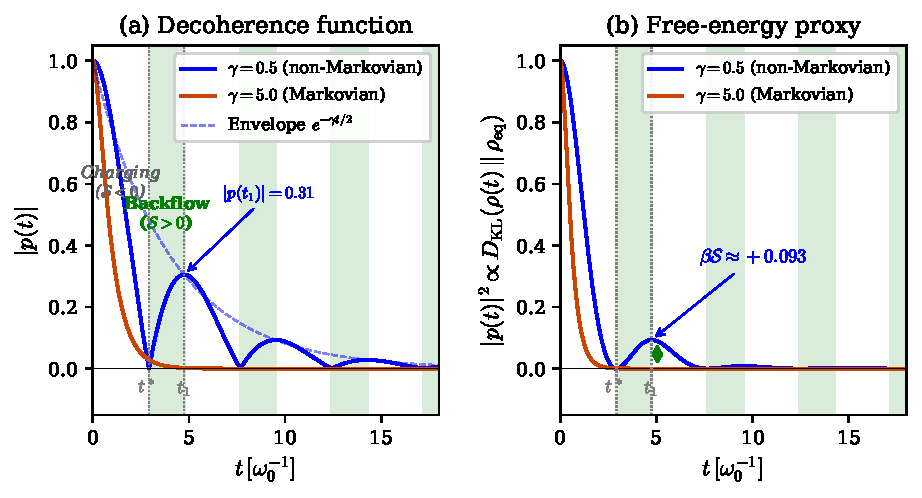
\includegraphics[width=\textwidth]{fig_survival.pdf}
\caption{%
Pure-dephasing spin-boson model
(Section~\ref{I-sec:example}) with Lorentz--Drude spectral
density~\eqref{I-eq:lorentz_drude}.
\textbf{Parameters:}
$\omega_0 = 1$ (energy unit),
$\lambda = 1$ (reorganization energy).
\textbf{Units:}
all times in $\omega_0^{-1}$;
energies in $\hbar\omega_0$.
\textbf{Regime:}
low temperature ($\beta\omega_0 \gg 1$);
the standard $T \to 0$ analytic
expression~\eqref{I-eq:decoherence}~\cite{BreuerPetruccione2002}
is used as an accurate proxy.
\textbf{(a)}~Decoherence amplitude $|p(t)|$
(eq.~\eqref{I-eq:decoherence}).
Blue: non-Markovian
($\gamma = 0.5$, $\gamma/4\lambda = 0.125$).
Orange: Markovian
($\gamma = 5.0$, $\gamma/4\lambda = 1.25$).
Dashed: exponential envelope $e^{-\gamma t/2}$.
Green bands indicate backflow
(Remark~\ref{I-rem:NM_regime}:
$d|p|/dt > 0$, $\Gamma(t) < 0$
per~\eqref{I-eq:Gamma_inst}).
\textbf{(b)}~Survival proxy
$|p(t)|^2 \propto \beta\,\mathcal{S}$
(eq.~\eqref{I-eq:S_qubit}).
At the first revival
($t_1 = \pi/\Omega \approx 4.75\,\omega_0^{-1}$),
the non-Markovian agent achieves
$\beta\,\mathcal{S}[t^*,t_1] \approx +0.093$
(eq.~\eqref{I-eq:S_numeric}), consistent with the
closed-form prediction~\eqref{I-eq:revival_exact},
funded by the consumption of pre-existing
correlations
(Proposition~\ref{I-prop:full_cycle}).
The Markovian comparison decays monotonically:
$\mathcal{S} \leq 0$ in this autonomous model
(Theorem~\ref{I-thm:autonomous_ceiling}).%
}
\label{I-fig:survival}
\end{figure}

\textbf{Consistency with
Theorem~\ref{I-thm:advantage} and
Proposition~\ref{I-prop:full_cycle}.}
Since this is autonomous evolution ($H_{\mathrm{ctrl}} = 0$),
identity~\eqref{I-eq:advantage_auto} applies exactly:
$\beta\,\mathcal{S} = -\Delta I(S{:}E)
- \Delta D_{\mathrm{KL}}(\rho_E \| \rho_E^{\mathrm{th}})$.
The example realizes the \emph{correlation battery}
of Remark~\ref{I-rem:battery}, with the charge--discharge
decomposition of
Proposition~\ref{I-prop:full_cycle}:
\begin{itemize}
\item \textbf{Charging} ($[0, t^*]$, eq.~\eqref{I-eq:charge}):
  the system decoheres, building correlations
  $I(S{:}E;\, t^*) > 0$ at the cost of
  $\mathcal{S} < 0$.
\item \textbf{Discharging} ($[t^*, t_1]$,
  eq.~\eqref{I-eq:discharge}):
  the correlations are consumed
  ($\Delta I < 0$ over this interval),
  returning $\beta\,\mathcal{S} \approx +0.093 > 0$.
\end{itemize}
The bound~\eqref{I-eq:S_upper} is satisfied:
$\beta\,\mathcal{S}[t^*, t_1] = 0.093
\leq I(S{:}E;\, t^*)$.
Full-cycle closure~\eqref{I-eq:full_cycle} is confirmed:
$\beta\,\mathcal{S}[0, t_1] < 0$.

\textbf{Instantaneous decoherence rate.}
The rate of coherence loss is
\begin{equation}
\label{I-eq:Gamma_inst}
\Gamma(t) := -\frac{d}{dt}\ln|p(t)|
= \frac{\gamma}{2}
  - \frac{\Omega\sin(\Omega t)
    + \tfrac{\gamma}{2}\cos(\Omega t)}
  {\cos(\Omega t)
    + \tfrac{\gamma}{2\Omega}\sin(\Omega t)}\,.
\end{equation}
In the Markovian limit $\gamma \gg 4\lambda$,
$\Gamma(t) \to \gamma/2 > 0$ for all $t$
(monotone decoherence).
In the non-Markovian regime $\gamma < 4\lambda$,
$\Gamma(t)$ oscillates and becomes \emph{negative}
during the backflow intervals where $|p(t)|$ increases.
These are precisely the intervals where
$\mathcal{S} > 0$.

\textbf{Closed-form revival amplitude.}
The decoherence function~\eqref{I-eq:decoherence} can be
written as $p(t) = R\, e^{-\gamma t/2}\cos(\Omega t - \phi)$,
where $R = \sqrt{1 + (\gamma/2\Omega)^2}$ and
$\phi = \arctan(\gamma/2\Omega)$, with $R\cos\phi = 1$.
The extrema of $|p(t)|$ occur at $t_n = n\pi/\Omega$
($n = 0, 1, 2, \ldots$), and the first revival peak
after the first zero is at $t_1 = \pi/\Omega$.
Its amplitude is \emph{exactly}
\begin{equation}
\label{I-eq:revival_exact}
|p(t_1)| = e^{-\gamma\pi/(2\Omega)},
\qquad
\beta\,\mathcal{S}[t^*, t_1]
\approx |p(t_1)|^2
= e^{-\gamma\pi/\Omega}.
\end{equation}
This is the paper's central computable prediction: the
survival gain at first backflow is determined by a single
dimensionless ratio $\gamma/\Omega$.

\begin{remark}[Parameter Survey]
\label{I-rem:parameter_survey}
Table~\ref{I-tab:survey} demonstrates the transition from
the Markovian regime ($\mathcal{S} \leq 0$) to the
non-Markovian regime ($\mathcal{S} > 0$) as the bath
memory rate $\gamma$ decreases below the critical value
$4\lambda$.
All entries use $\omega_0 = 1$, $\lambda = 1$,
$W = 0$ (autonomous evolution), with revival amplitudes
computed from~\eqref{I-eq:revival_exact}.
\begin{center}
\begin{tabular}{@{}cccccc@{}}
\toprule
$\gamma$ & $\gamma/4\lambda$ & Regime
& $|p(t_1)|$ & $\beta\,\mathcal{S}(t_1)$
& $\Gamma_{\min}$ \\
\midrule
$20.0$ & $5.0$ & Markov & --- & $\leq 0$ & $>0$ \\
$4.0$ & $1.0$ & Critical & --- & $\leq 0$ & $= 0$ \\
$2.0$ & $0.50$ & Non-Markov & $0.043$
  & $+0.002$ & $< 0$ \\
$1.0$ & $0.25$ & Non-Markov & $0.163$
  & $+0.027$ & $< 0$ \\
$0.5$ & $0.125$ & Deep NM & $0.305$
  & $+0.093$ & $< 0$ \\
$0.1$ & $0.025$ & Deep NM & $0.605$
  & $+0.37\phantom{0}$ & $< 0$ \\
\bottomrule
\end{tabular}
\end{center}
\captionsetup{hypcap=false}%
\captionof{table}{%
Survival functional at first backflow revival
as a function of the bath memory rate $\gamma$,
for the pure-dephasing spin-boson model
with Lorentz--Drude spectral density.
$|p(t_1)|$ is computed
from~\eqref{I-eq:revival_exact};
$\Gamma_{\min}$ is the sign of the minimum of the
instantaneous decoherence rate~\eqref{I-eq:Gamma_inst}.
The transition $\mathcal{S} \leq 0 \to \mathcal{S} > 0$
occurs precisely at the non-Markovian threshold
$\gamma = 4\lambda$.
For $\gamma = 0.1$ (deep non-Markovian),
the agent achieves $\beta\,\mathcal{S} \approx +0.37$
per backflow cycle in the autonomous setting
($H_{\mathrm{ctrl}} = 0$).%
}
\label{I-tab:survey}
\end{remark}

\begin{remark}[The Two Regimes: Summary]
\label{I-rem:two_regimes}
\begin{center}
\begin{tabular}{@{}lll@{}}
\toprule
& \textbf{Markovian ($\gamma = 20$)}
& \textbf{Non-Markovian ($\gamma = 0.5$)} \\
\midrule
$\gamma / 4\lambda$ & $5.0$ (overdamped)
  & $0.125$ (underdamped) \\
$\tau_B$ & $0.05\,\omega_0^{-1}$
  & $2.0\,\omega_0^{-1}$ \\
$p(t)$ & Monotone decay
  & Oscillatory with envelope \\
$|p(t_1)|$ at first revival & $0$ (no revival)
  & $\approx 0.31$ \\
$\beta\,\mathcal{S}$ at revival & $\leq 0$
  & $\approx +0.093$ \\
$\Gamma(t)$ & $> 0$ always
  & Oscillates, $< 0$ during backflow \\
Interpretation & Stone (sinks)
  & Surfer (rides backflow) \\
\bottomrule
\end{tabular}
\end{center}
The non-Markovian agent achieves
$\beta\,\mathcal{S} \approx +0.093$
per backflow cycle (autonomous, $H_{\mathrm{ctrl}} = 0$),
while the Markovian agent can only lose free energy.
As the coupling deepens ($\gamma/4\lambda \to 0$), the
revival amplitude grows and
$\mathcal{S}$ increases
(Table~\ref{I-tab:survey}), bounded above by
$\beta\,\mathcal{S} \leq I(S{:}E;\, t^*)$
(Corollary~\ref{I-cor:three_regimes}(iii)).
\end{remark}

% ============================================================
\section{The Cost of Memory}
\label{I-sec:cost}

The preceding identity allows a correlated initial resource to fund a
later interval.  It does not assign a universal energetic price to
storing or maintaining that resource.  This section separates
Landauer's erasure bound from a conditional archive-overload model used
only to motivate Paper~II.

\subsection{The Landauer Debt}

Landauer's principle prices a logically irreversible reset, not passive
storage, sensing, correlation maintenance, or reversible computation.

\begin{remark}[Conditional erasure cost]
\label{I-rem:landauer_scope}
If a declared memory implementation irreversibly erases
$N_{\mathrm{erase}}$ unbiased bits into a bath at temperature $T$, its
reset work obeys
\begin{equation}
\label{I-eq:landauer}
W_{\mathrm{reset}}\geq k_BT\ln2\,N_{\mathrm{erase}}.
\end{equation}
No lower bound proportional to total stored mutual information follows
without an implementation model.  Reversible storage and reversible
measurement can in principle avoid this reset cost until a logically
irreversible operation is performed~\cite{Landauer1961,Bennett1982}.
The former universal ``Landauer Cost of Memory'' proposition is
withdrawn.
\end{remark}

\subsection{Raw Archive Overload Scenario}

The crisis arises from the scaling of
$\mathcal{I}_{\mathrm{stored}}$ with time.
To quantify this, we borrow two quantities from computational
mechanics~\cite{CrutchfieldYoung1989,ShaliziCrutchfield2001}:

\begin{definition}[Entropy Rate and Predictive Information]
\label{I-def:entropy_rate}
Let $\{X_t\}$ be the stochastic process describing the
environment's influence on the agent (e.g., the sequence of
bath correlation values).
\begin{enumerate}
\item The \textbf{entropy rate} of the environment is
  \begin{equation}
  \label{I-eq:entropy_rate}
  h_\mu := \lim_{n \to \infty}
  H(X_n \mid X_{n-1}, \ldots, X_1),
  \end{equation}
  measuring the intrinsic unpredictability per time step.
\item The \textbf{predictive information} (excess entropy) is
  \begin{equation}
  \label{I-eq:pred_info}
  I_{\mathrm{pred}} := I(\overleftarrow{X};\,
  \overrightarrow{X})
  = \sum_{k=1}^{\infty}
  \bigl[H(X_k) - h_\mu\bigr],
  \end{equation}
  where $\overleftarrow{X}$ and $\overrightarrow{X}$ denote
  the past and future half-chains.
  This is the total amount of information about the future
  that is encoded in the past---the \emph{useful} memory.
\end{enumerate}
\end{definition}

Finite predictive information does not by itself prove that a finite
physical memory captures every useful feature, and positive entropy
rate does not lower-bound predictive information by
$h_\mu\tau_{\mathrm{mem}}$.  In particular, a stationary mixing
process commonly has finite excess entropy.

\begin{remark}[Conditional archive-overload scenario]
\label{I-rem:archive_overload}
Consider a deliberately specified implementation: an uncompressed raw
archive receives records at rate $r_{\mathrm{raw}}$ bits per unit time,
has capacity $M$ bits, and evaluates the entire archive once per control
cycle.  Without deletion it fills after $M/r_{\mathrm{raw}}$.  If it
irreversibly resets discarded records at rate $r_{\mathrm{erase}}$,
Landauer gives
\begin{equation}
\label{I-eq:mem_cost_rate}
\dot W_{\mathrm{reset}}\geq
k_BT\ln2\,r_{\mathrm{erase}}.
\end{equation}
For a long-memory or non-stationary source with divergent
$I_{\mathrm{pred}}$, the amount of predictively relevant history may
also grow, but that is an additional source assumption.  This archive
can exceed a finite storage, throughput, or reset budget.  The result is
an engineering overload scenario, not a universal thermodynamic
catastrophe and not a theorem that every memory implementation must
compress.
\end{remark}

\subsection{Conditional Motivation for Compression}

An agent using the raw-archive implementation may respond by increasing
capacity, lowering sample rate, reversible uncomputation, sufficient
statistics, lossy compression, or accepting stale data.  Paper~II
studies one coordinate-selection model among these options.

\begin{itemize}
\item \textbf{Compression requires a criterion.}
  To decide what to keep and what to erase, the agent needs a
  \emph{relevance function}---a mapping from stored correlations
  to survival value.
  This is a reference frame that ranks information by its
  contribution to $\mathcal{S}$.

\item \textbf{Coordinate selection uses a reference frame.}
  If the admissible compressor is restricted to retaining a subset of
  supplied coordinates, choosing that subset privileges a basis.  More
  general invariant or learned sufficient-statistic compressors need
  not have this form.
\end{itemize}

\begin{remark}[The Origin of Paper II]
\label{I-rem:paper_II}
Remark~\ref{I-rem:archive_overload} supplies Paper~II with a conditional
motivation: a bounded agent attempting to evaluate an uncompressed
archive needs some resource-allocation policy.  It does not prove that
compression, Clifford coordinates, spontaneous symmetry breaking, or a
``self'' is thermodynamically necessary.  Those are modelling choices
to be assessed in Paper~II.
\end{remark}

% ============================================================
\section{Numerical Demonstration}
\label{I-sec:numerical}

The preceding sections establish an autonomous thermodynamic baseline
and an accounting identity.  The following HMM is a separate classical
performance illustration: it compares finite observation windows with
a Bayes filter in an aliased environment.  Reward here is not the
thermodynamic survival functional, so the demonstration does not test
either theorem.
Full code and parameters are provided for reproducibility.

% ------------------------------------------------------------
\subsection{Model}
\label{I-subsec:demo_model}

\paragraph{Environment.}
A two-hidden-state HMM with aliased observations.
The hidden state $s_t \in \{0,1\}$ evolves as a persistent
Markov chain with $\Pr(s_{t+1} = s_t) = 1 - \varepsilon$;
the parameter $\varepsilon \in [10^{-3}, 10^{-1}]$ controls
the correlation length $\ell \sim 1/\varepsilon$.
Observations $o_t \in \{A, B\}$ are aliased:
$\Pr(o_t = A \mid s_t = 0) = 0.5 + \delta$,
$\Pr(o_t = A \mid s_t = 1) = 0.5 - \delta$,
with $\delta = 0.05$ (mutual information
$I(O; S) \approx 0.007$~bits).
Reward: $r_t = 1$ if $a_t = s_t$, $0$ otherwise.

\paragraph{Agents.}
All agents use the true model parameters and compute
exact Bayesian posteriors; the only difference is how many
observations each agent retains.
\begin{itemize}
\item \textbf{Markov-$k$} ($k \in \{1,2,4,8\}$): runs
  an exact Bayes filter over the most recent $k$
  observations (sliding window, uniform prior at each
  window start); acts by MAP.
\item \textbf{Memory (Bayes filter)}: maintains the full
  belief state $b_t = \Pr(s_t = 1 \mid o_{1:t})$ via the
  exact predict--update cycle over all past observations;
  acts by MAP.
\end{itemize}

\paragraph{Parameters.}
\begin{center}
\small
\begin{tabular}{@{}lcl@{}}
\toprule
\textbf{Quantity} & \textbf{Value} & \textbf{Role} \\
\midrule
$T$ & $100{,}000$ & horizon per trial \\
Seeds & 10 & independent replications \\
$\delta$ & 0.05 & observation asymmetry \\
$k$ & $\{1, 2, 4, 8\}$ & Markov window sizes \\
$\varepsilon$ & logspace($10^{-3}$, $10^{-1}$, 15)
  & transition noise grid \\
Burn-in & $5{,}000$ & discarded steps \\
\bottomrule
\end{tabular}
\end{center}

% ------------------------------------------------------------
\subsection{Results}
\label{I-subsec:demo_results}

Figure~\ref{I-fig:markov_ceiling} shows the two key signatures.

\paragraph{Result 1: finite-window performance saturation
(Figure~\ref{I-fig:markov_ceiling}a).}
The average reward $\bar{R}$ of the Bayes filter (memory
agent) increases monotonically with correlation length
$\ell = 1/\varepsilon$, while each Markov-$k$ agent
saturates at a distinct ceiling.  The ceilings are
ordered: $k = 1$ (lowest) through $k = 8$ (highest),
and all fall below the memory agent for
$\ell \gtrsim 20$.  This is a property of the specified
aliased HMM and agent classes, not a consequence of the
thermodynamic ceiling.

\paragraph{Result 2: Memory advantage
(Figure~\ref{I-fig:markov_ceiling}b).}
The gap $\Delta\bar{R} = \bar{R}_{\mathrm{mem}}
- \bar{R}_{\mathrm{Markov}\text{-}k}$ increases
monotonically with $\ell$, and is larger for smaller $k$.
Shaded bands show 95\% confidence intervals across
10 seeds.  The Markov-1 and Markov-2 curves nearly
overlap at small $\ell$, reflecting the fact that
short observation windows provide negligible additional
information in this aliasing regime---a consistency
check, not a deficiency.

\begin{figure}[t]
\centering
\includegraphics[width=\textwidth]%
  {fig_paper1_markov_ceiling.pdf}
\caption{%
\textbf{Finite-window saturation and Bayes-filter advantage.}
$T = 100{,}000$, 10 seeds, 95\% CI bands.
\textbf{(a)}~Average reward $\bar{R}$ vs correlation
length $\ell = 1/\varepsilon$.  The Bayes filter
(blue, bold) rises monotonically; Markov-$k$ agents
saturate at $k$-dependent ceilings.
\textbf{(b)}~Performance gap
$\Delta\bar{R} = \bar{R}_{\mathrm{mem}}
- \bar{R}_{\mathrm{Markov}\text{-}k}$
increases with $\ell$; smaller $k$ yields a larger gap.}
\label{I-fig:markov_ceiling}
\end{figure}

% ------------------------------------------------------------
\subsection{Scope of This Demonstration}
\label{I-subsec:demo_scope}

These simulations illustrate finite-window saturation under the stated
model class; they do not constitute a thermodynamic test.

\medskip
This demonstration \textbf{does} show:
\begin{enumerate}
\item A reproducible regime in which finite-order Markov
  agents exhibit a performance ceiling while a
  memory-carrying (Bayes filter) agent improves.
\item The performance gap widens with correlation length and tightens
  with window size in this HMM.  This is conceptually related to
  retained history but is not the quantity in
  Theorem~\ref{I-thm:advantage}.
\end{enumerate}

\noindent
This demonstration does \textbf{not} show:
\begin{enumerate}
\item Universality across environments, observation models,
  or agent architectures.  The model uses a two-state
  HMM with binary aliased observations.
\item Tight constants or the functional form of the
  ceiling boundary $\ell_c(k)$.
\item That the Bayes filter is optimal among all possible
  memory-carrying agents.
\end{enumerate}

\paragraph{Reproducibility.}
\begin{sloppypar}
The complete simulation is a self-contained Python script
(\texttt{paper1\_markov\_ceiling\_demo.py}, ${\sim}\,560$
lines, requiring only NumPy and Matplotlib) with fixed
random seeds.  All figures in this section can be
reproduced by executing the script.  The following files
are included in the supplementary archive:
\begin{itemize}
\item \texttt{paper1\_markov\_ceiling\_demo.py} --- simulation script
\item \texttt{fig\_paper1\_markov\_ceiling.pdf} --- Figure~\ref{I-fig:markov_ceiling}
\item \texttt{markov\_ceiling\_data.csv} --- raw sweep data
\item \texttt{markov\_ceiling\_boundary.csv} --- extracted
  ceiling boundaries $\ell_c(k)$
\end{itemize}
\end{sloppypar}

% ============================================================
\section{Discussion}
\label{I-sec:discussion}

\subsection{Summary of Results}

\begin{center}
\small
\setlength{\tabcolsep}{4pt}%
\begin{tabular}{@{}lP{7.5cm}c@{}}
\toprule
\textbf{Result} & \textbf{Statement} & \textbf{Sec.} \\
\midrule
Restricted autonomous ceiling &
  $\mathcal{S} \leq 0$ for a fixed-Hamiltonian Davies semigroup
  & \ref{I-sec:ceiling} \\[3pt]
Initial-resource balance &
  $\beta\mathcal{S} = -\Delta I
  - \Delta D_{\mathrm{KL}}
  - \beta\Delta\langle H_{\mathrm{ctrl}}\rangle
  - \beta\Delta\langle H_{\mathrm{int}}\rangle$
  & \ref{I-sec:advantage} \\[3pt]
Quantitative demo &
  Spin-boson: $\beta\mathcal{S} \approx +0.093 > 0$
  at first backflow revival (Fig.~\ref{I-fig:survival},
  Table~\ref{I-tab:survey})
  & \ref{I-sec:example} \\[3pt]
Memory/record interface &
  operational influence relation plus a conditional record test
  & \ref{I-sec:arrow} \\[3pt]
Archive overload &
  conditional on raw storage, finite capacity, and irreversible reset
  & \ref{I-sec:cost} \\[3pt]
Numerical demo &
  finite-window saturation in an aliased HMM
  (Fig.~\ref{I-fig:markov_ceiling})
  & \ref{I-sec:numerical} \\
\bottomrule
\end{tabular}
\end{center}

\subsection{What This Paper Does and Does Not Show}

\textbf{This paper shows:}
\begin{enumerate}
\item Under an autonomous fixed-Hamiltonian Davies semigroup,
  the survival functional $\mathcal{S} \leq 0$
  (Theorem~\ref{I-thm:autonomous_ceiling}).
\item For any initial state (product or correlated), the
  survival functional satisfies the exact identity
  $\beta\,\mathcal{S} = -\Delta I(S{:}E)
  - \Delta D_{\mathrm{KL}}(\rho_E \| \rho_E^{\mathrm{th}})
  - \beta\,\Delta\langle H_{\mathrm{ctrl}}\rangle
  - \beta\,\Delta\langle H_{\mathrm{int}}\rangle$
  (Theorem~\ref{I-thm:advantage}).
  Under autonomous evolution, when pre-existing
  system--environment correlations are consumed
  ($\Delta I < 0$), $\mathcal{S} > 0$ is achievable,
  bounded by the initial correlation budget
  (Corollary~\ref{I-cor:three_regimes}).
\item A quantitative spin-boson example illustrates:
  $\beta\,\mathcal{S} \approx +0.093 > 0$ at the first
  non-Markovian revival (Section~\ref{I-sec:example}).
\item The memory-influence relation and HAFF record ordering define a
  conditional model test, not a proved embedding
  (Conjecture~\ref{I-prop:HAFF_bridge}).
\item Landauer supplies a conditional reset cost; a raw finite archive
  can overload under the implementation assumptions in
  Remark~\ref{I-rem:archive_overload}.
\item A computational demonstration exhibits finite-window saturation
  in a two-state HMM with aliased observations
  (Section~\ref{I-sec:numerical},
  Figure~\ref{I-fig:markov_ceiling}).
\end{enumerate}

\textbf{This paper does not show:}
\begin{enumerate}
\item That memory or non-Markovianity is necessary or sufficient for
  persistence.
\item That non-Markovian systems optimize a larger survival supremum
  than all Markovian systems.
\item That driven or measurement-feedback Markovian agents obey the
  restricted autonomous ceiling (Remark~\ref{I-rem:driven_protocol}).
\item That the specific form of the optimal memory kernel can be
  derived from first principles without specifying the
  environment.
\item That memory implies or requires consciousness.
\item That storage or maintenance has a universal Landauer cost, or
  that compression and symmetry breaking are thermodynamic necessities.
\end{enumerate}

% ============================================================
% REFERENCES
% ============================================================

% ============================================================================
% Paper II --- ``The Ego''
% ============================================================================
\chapter{Spontaneous Symmetry Breaking of Reference Frames as a Computational Cost Minimization Strategy}
\label{chap:paperII}

\begin{center}
\textit{Paper II --- ``The Ego''}\\[0.5em]
Originally published: Zenodo, DOI: 10.5281/zenodo.18579703
\end{center}

\bigskip

\section*{Abstract}
We investigate a conditional implementation model for bounded agents
that process memory-like state under finite computational resources.
Revised Paper~I~\cite{Liu2026TDOME_I} supplies a conditional
correlation-resource account; it does not establish universal memory
necessity, a universal Markovian ceiling, or a Landauer charge for
merely storing records.

The present paper therefore studies a declared raw $D$-channel archive
processed under a finite throughput budget.  Within that model,
symmetric processing of all declared channels can exceed the available
budget at a finite time, while a supplied coordinate selector can reduce
the declared load.  This is a conditional overload result for the stated
archive and algorithm, not a theorem that every persistent agent must
compress memory or break a symmetry.

Reference-frame selection is treated as a modelling strategy: a
privileged basis or coordinate projection packages a lower-dimensional
representation of the archive.  The rate-distortion calculation gives a
budget-dependent target dimension under the stated source, distortion,
and budget assumptions.  It does not prove that the ``self'' is a
universal survival-optimal structure.

The projected representation is accompanied by four diagnostic labels:
basis selection, frame drag, objective centering, and model
incompleteness.  Only basis selection follows from projection alone; the
other diagnostics require additional controller, update, objective, or
task assumptions.  A simple drift model gives a visibility crossover for
a fixed frame, motivating Paper~III's calibration problem without
establishing an undetectable universal Delusion Trap.


% ============================================================
\section{Introduction}
\label{II-sec:intro}

% ------------------------------------------------------------
\subsection{Context: The Problem of Overload}
\label{II-subsec:overload}

Revised Paper~I~\cite{Liu2026TDOME_I} gives an ELV-type
accounting identity in which initial correlations can fund a later
interval and proves a ceiling only for a fixed-Hamiltonian autonomous
Davies baseline.  It retracts both universal memory necessity and a
Landauer charge for merely storing or maintaining records.

The present paper therefore begins with an independent implementation
model: a raw, uncompressed $D$-channel archive processed under a finite
throughput budget.  Its overload is conditional on that archive and
algorithm.  The question is when a supplied coordinate selector can
reduce this declared load, not whether every persistent agent must
compress or break symmetry.

% ------------------------------------------------------------
\subsection{Position within the Series}
\label{II-subsec:series_position}

This paper is the second of three constituting the
\textbf{T-DOME} (Thermodynamic Dynamics of Observer-Memory
Entanglement) framework, the third pillar of a three-paper
program.

\begin{center}
\small
\setlength{\tabcolsep}{4pt}%
\begin{tabular}{@{}lP{3.2cm}cP{3.4cm}c@{}}
\toprule
\textbf{Framework} & \textbf{Question} & & \textbf{Result}
  & \textbf{Status} \\
\midrule
HAFF~\cite{Liu2026HAFF_A,Liu2026HAFF_B}
  & How does geometry emerge?
  & Ocean
  & Conditional algebra/dictionary models
  & Revised \\[3pt]
Q-RAIF~\cite{Liu2026QRAIF_A,Liu2026QRAIF_B}
  & What algebra must an observer have?
  & Fish
  & Clifford representation as model input
  & Revised \\[3pt]
T-DOME~I~\cite{Liu2026TDOME_I}
  & What can inter-epoch correlations fund?
  & Seed
  & Restricted baseline; accounting identity
  & Conditional \\[3pt]
\textbf{T-DOME~II} (this work)
  & When can a model select a frame?
  & Ego
  & Conditional coordinate selection
  & \textbf{This paper} \\[3pt]
T-DOME~III
  & When can residual statistics track drift?
  & Loop
  & Conditional Fisher calibration
  & Companion \\
\bottomrule
\end{tabular}
\end{center}

The three T-DOME papers form a conditional modelling sequence rather
than an irreversible theorem chain:
\begin{enumerate}
\item \textbf{Paper~I (The Seed):} An ELV-type balance identifies
  initial correlations as one possible interval resource.  Raw-archive
  overload is an implementation scenario, not a thermodynamic
  necessity.
\item \textbf{Paper~II (The Ego, this work):} Unbounded memory
  under finite computational resources causes processing
  overload in the coordinate-processing model.  This paper studies
  conditional feature selection; it does not prove universal SSB.
\item \textbf{Paper~III (The Loop):} Uncorrected bias diverges
  from a changing environment. A self-referential calibration
  loop (monitoring one's own prediction error) resolves the
  bias but requires the system to ``observe its own
  observation''---closing the self-calibration loop.
\end{enumerate}

% ------------------------------------------------------------
\subsection{Relation to Q-RAIF}
\label{II-subsec:qraif}

Revised Q-RAIF Papers A and B~\cite{Liu2026QRAIF_A,Liu2026QRAIF_B}
use a Clifford algebra $Cl(V,q)$ as a supplied representation choice;
persistence does not select it.  Paper C~\cite{Liu2026QRAIF_C} proves
only that the image of a separately supplied homomorphism lies in the
external algebra.  This paper adopts both the Clifford coordinates and
the representation map as model inputs.

The Clifford algebra $Cl(V,q)$, however, admits a non-trivial
\emph{automorphism group} $G = \mathrm{Aut}(Cl(V,q))$.
In the absence of external constraints, all elements of $G$
yield physically equivalent representations---the choice of
basis within the algebra is a \emph{gauge freedom}.
This gauge freedom is the mathematical substrate of the
symmetry considered in the conditional breaking analysis below.

The ``ego'' names a selected computational frame in that supplied
representation.  Whether a concrete optimum is a genuine gauge fixing
is a model condition, not an inherited theorem.

% ------------------------------------------------------------
\subsection{Relation to HAFF Paper~G}
\label{II-subsec:haff_g}

Revised HAFF Paper~G~\cite{Liu2026HAFF_G} offers
philosophy-of-science motivation and no fixed-point no-go theorem.  It
does not imply basis selection here.  Any connection between its
meta-level concern and this finite-budget model is motivation only.

% ------------------------------------------------------------
\subsection{Scope and Disclaimers}
\label{II-subsec:scope}

To prevent interpretational overreach, we state at the
outset what this paper does \emph{not} claim:
\begin{enumerate}
\item We do not claim that symmetry breaking is
  \emph{sufficient} for persistence.
  Paper~III addresses the additional requirements.
\item We do not claim that basis selection or spontaneous symmetry
  breaking is necessary for every bounded agent.  The results concern
  a declared coordinate-retention model.
\item The term ``ego'' or ``self'' is used in the
  control-theoretic sense: a fixed reference frame within
  the agent's internal algebra. It carries no implication
  of consciousness or subjective experience.
\item A broader structural analogy with classical philosophical
  concepts of selfhood exists but is outside the scope of
  this paper.
\end{enumerate}

\paragraph{Related work.}
The idea that bounded agents must compress their
representations has roots in Simon's bounded
rationality~\cite{Simon1955}, Shannon's
rate-distortion theory~\cite{Shannon1959,CoverThomas2006},
and Sims's rational inattention~\cite{Sims2003}, which
models finite-capacity decision-makers as solving a
rate-distortion problem---precisely the economic
counterpart of our $\mathcal{C}_{\mathrm{budget}}$
formalism.
The information bottleneck~\cite{Tishby2000}
formalises relevance-weighted compression and has been
applied to neural coding and deep
learning.
The role of decoherence in selecting preferred bases
(pointer states) is well established via quantum
Darwinism~\cite{Zurek2009}; here it motivates one
model-specific coordinate-selection rule.
Measures of non-Markovianity and their thermodynamic
consequences are reviewed
in~\cite{RivasHuelgaPlenio2014,BreuerPetruccione2002};
the connection to survival was established in Paper~I.

\paragraph{Summary of contributions.}
This paper separates three levels of result:
\begin{enumerate}
\item \textbf{Raw-channel load scaling law}
  a conditional accounting identity for a raw $D$-channel archive.
\item \textbf{Survival-weighted rate-distortion bound}
  a compactness-based existence result; the budget supplies only a
  capacity $k_{\max}$, not a universal optimal retained dimension.
\item \textbf{Delusion dynamics}
  a linear-drift visibility crossover plus an explicit two-mode
  example showing when gradient anti-correlation can occur.
\end{enumerate}

\paragraph{Result-status ledger.}
The original Computational Ceiling and SSB-necessity chain is retracted
(`TD-II-T3.5`).  Raw-channel load is an FD/I accounting proposition;
compression existence is conditional on a compact feasible model; SSB
is a model interpretation.  The Delusion Trap is downgraded
(`TD-II-T6.7`): visibility crossover is exact in the declared two-mode
geometry, while gradient sign and self-detection require extra dynamics.

% ============================================================
\section{Mathematical Preliminaries}
\label{II-sec:prelim}

% ------------------------------------------------------------
\subsection{Inherited Framework from Paper~I}
\label{II-subsec:inherited}

We briefly recall the key objects from
Paper~I~\cite{Liu2026TDOME_I} that the present work builds
upon.  The reader is referred to Paper~I for full definitions
and proofs.

\paragraph{Survival functional.}
For an open quantum system $S$ coupled to an environment $E$
at inverse temperature $\beta$, with dynamics $\Lambda$ and
external control protocol $H_{\mathrm{ctrl}}(t)$, the
survival functional is
\begin{equation}
\label{II-eq:survival_recall}
\mathcal{S}[\Lambda, \tau]
:= \Delta F - W[0,\tau],
\end{equation}
where $\Delta F = F(\rho(\tau)) - F(\rho(0))$ is the change
in non-equilibrium free energy and
$W = \int_0^\tau \tr(\rho(t)\,\dot{H}_{\mathrm{ctrl}}(t))\,dt$
is the work performed by the external protocol.

\paragraph{Restricted autonomous baseline.}
For a fixed-Hamiltonian Davies semigroup with no control, Paper~I proves
\begin{equation}
\label{II-eq:ceiling_recall}
\mathcal{S}[\Lambda^{\mathrm{M}}, \tau] \leq 0
\qquad\text{for all } \tau \geq 0.
\end{equation}
It does not extend this result to driven Markovian agents.

\paragraph{Non-Markovian advantage identity.}
For arbitrary initial states:
\begin{equation}
\label{II-eq:advantage_recall}
\beta\,\mathcal{S}
= -\Delta I(S{:}E)
  - \Delta D_{\mathrm{KL}}(\rho_E \| \rho_E^{\mathrm{th}})
  - \beta\,\Delta\langle H_{\mathrm{ctrl}} \rangle
  - \beta\,\Delta\langle H_{\mathrm{int}} \rangle.
\end{equation}

\paragraph{Conditional raw-archive model.}
Paper~I retracts a universal Landauer maintenance bound.  This paper
independently posits an uncompressed record stream.  Let $h_\mu$ be its
\emph{per-component} entropy rate~\cite{CrutchfieldYoung1989},
defined by
\begin{equation}
\label{II-eq:entropy_rate}
h_\mu
:= \lim_{T\to\infty}\frac{1}{T}\,H(X_{0:T}),
\end{equation}
measuring the asymptotic information (in bits per unit time)
generated by one declared record channel (we work in units where the sampling interval equals
the environmental correlation time
$\tau_E$)\footnote{For a continuous-valued process sampled at
resolution $b$ bits, $h_\mu$ includes the quantisation cost:
$h_\mu = h_\mu^{(\mathrm{diff})} + b\,f_s$, where
$h_\mu^{(\mathrm{diff})}$ is the differential entropy rate
and $f_s$ the sampling frequency.  All raw-channel accounting
identities in this paper use $h_\mu$ so defined.}
The predictive information
$I_{\mathrm{pred}}$ is the \emph{excess entropy}
(excess entropy)~\cite{BialekNemenmanTishby2001,ShaliziCrutchfield2001},
defined as the mutual information between past and future
of the environmental process:
\begin{equation}
\label{II-eq:I_pred}
I_{\mathrm{pred}}
:= I\!\left(\overleftarrow{X};\, \overrightarrow{X}\right)
= H(\overrightarrow{X})
  - H(\overrightarrow{X} \mid \overleftarrow{X}),
\end{equation}
where $\overleftarrow{X}$ and $\overrightarrow{X}$ denote
the semi-infinite past and future, respectively.
For a stationary process,
$I_{\mathrm{pred}}$ relates to $h_\mu$ via the entropy-rate
decomposition
$H(X_{1:T}) = I_{\mathrm{pred}} + h_\mu\,T + o(1)$
as $T \to \infty$ when the relevant limits exist
\cite{CrutchfieldYoung1989}.  No lower bound
$I_{\mathrm{stored}}\geq\min(I_{\mathrm{pred}},h_\mu\tau)$
is inherited.

% ------------------------------------------------------------
\subsection{The Agent's Internal Algebra}
\label{II-subsec:algebra}

As a modelling choice motivated by revised
Q-RAIF~\cite{Liu2026QRAIF_B,Liu2026QRAIF_C},
the agent's internal control algebra is taken to be a Clifford algebra
$\mathcal{O}_{\mathrm{int}} = Cl(V,q)$
for a real vector space $V$ equipped with a non-degenerate
quadratic form $q$.
The algebra satisfies the fundamental relation
$v^2 = q(v)\,\mathbf{1}$ for all $v \in V$.

The \emph{automorphism group}
\begin{equation}
\label{II-eq:gauge_group}
G := \mathrm{Aut}(Cl(V,q))
\end{equation}
is the group of algebra automorphisms that preserve the
grading and quadratic form.\footnote{\label{II-fn:gauge_group}%
We use $G$ as an effective symmetry group acting
transitively on admissible frames.
The detailed Lie-algebraic structure of $G$ is not required
for our results; only the existence of a non-trivial
symmetry that may be broken under the additional encoder
conditions in Remark~\ref{II-rem:conditional_ssb}.
In concrete models, one may replace $G$ by its image
under the adjoint representation---typically
$O(V,q)$ or a pin/spin subgroup.}
For $Cl(1,3)$, $G$ contains the spin group
$\mathrm{Spin}(1,3) \cong SL(2,\mathbb{C})$
as a subgroup---a six-real-dimensional Lie group.

In the absence of computational constraints, all
$g \in G$ yield physically equivalent descriptions of
the agent's internal state.
The choice of basis within $Cl(V,q)$ is a \emph{gauge
freedom}---the symmetry examined in the conditional
coordinate-selection model below.

A representation map
$\phi:Cl(V,q)\to\mathcal A_{\mathrm{ext}}$ is supplied as an
interface.  Q-RAIF Paper C proves only the image-level algebraic
statement once this map is given; it does not select a preferred
$Cl(1,3)$ target or preserve quadratic signature.

\paragraph{Dimensional convention.}
Two distinct notions of dimension appear throughout:
\begin{center}
\small
\begin{tabular}{@{}lll@{}}
\toprule
Symbol & Meaning & Scaling \\
\midrule
$n := \dim V$ & number of generators
  (degrees of freedom) & --- \\
$D := \dim Cl(V,q) = 2^n$ & full multivector space
  (algebra basis size) & exponential in $n$ \\
\bottomrule
\end{tabular}
\end{center}
The raw-channel load model (Section~\ref{II-sec:ceiling})
scales with~$D$, not~$n$; the distinction matters
whenever one compares generator-level and
algebra-level quantities.

% ------------------------------------------------------------
\subsection{Rate-Distortion Theory}
\label{II-subsec:RD}

We require the classical rate-distortion framework
of Shannon~\cite{Shannon1959}.

\begin{definition}[Rate-distortion function]
\label{II-def:RD}
Let $X$ be a random source with distribution $p(x)$,
$\hat{X}$ a reconstruction, and
$d: \mathcal{X} \times \hat{\mathcal{X}} \to [0,\infty)$
a distortion measure.
The \emph{rate-distortion function} is
\begin{equation}
\label{II-eq:RD}
R(D) := \min_{\substack{p(\hat{x}|x):\\
  \mathbb{E}[d(X,\hat{X})] \leq D}} I(X; \hat{X}),
\end{equation}
the minimum mutual information between source and
reconstruction that achieves average distortion at most $D$.
\end{definition}

$R(D)$ is a convex, non-increasing function of $D$ with
$R(0) = H(X)$ (lossless) and
$R(D_{\max}) = 0$ (maximum distortion).
It provides the fundamental limit on lossy
compression~\cite{CoverThomas2006}.
The \emph{information bottleneck} method of
Tishby et al.~\cite{Tishby2000} generalises this framework
to the case where the relevant variable is not the source
itself but a downstream prediction target---precisely the
situation in our survival-weighted compression problem
(Section~\ref{II-subsec:RD_bound}).
For source $X$, representation $Z$, and declared survival-relevant
target $Y$, the bottleneck objective is
\begin{equation}
\min_{p(z|x)} I(X;Z)-\beta_{\mathrm{IB}} I(Z;Y).
\end{equation}
The coordinate-retention model below does not solve this unrestricted
optimization.  Rate-distortion and information bottleneck therefore
provide comparison frameworks, not authority for the component count.

% ------------------------------------------------------------
\subsection{Bounded Rationality}
\label{II-subsec:bounded}

Following Simon~\cite{Simon1955}, we model computational
limitations as a hard constraint on the agent's information
processing rate.

\begin{definition}[Computational budget]
\label{II-def:budget}
The agent's \emph{computational budget}
$\mathcal{C}_{\mathrm{budget}}$ (measured in bits per unit
time) is the maximum rate at which the agent can evaluate
functions of its stored correlations.
We assume $\mathcal{C}_{\mathrm{budget}} < \infty$.
\end{definition}

Physically, finiteness of $\mathcal{C}_{\mathrm{budget}}$
reflects the finite number of degrees of freedom in the
agent's physical substrate: finite Hilbert space dimension,
finite memory register size, and finite energy available for
computation (Landauer's
principle~\cite{Landauer1961,Bennett1982}).

% ------------------------------------------------------------
\subsection{Fiber Bundle Formalism}
\label{II-subsec:fiber}

The geometric setting for reference-frame selection is a
principal fiber bundle.

\begin{definition}[Gauge bundle]
\label{II-def:bundle}
The \emph{gauge bundle} is the principal $G$-bundle
\begin{equation}
\label{II-eq:bundle}
\pi: P \to M, \qquad G = \mathrm{Aut}(Cl(V,q)),
\end{equation}
where:
\begin{itemize}
\item $M$ is the base space of \emph{effective memory
  kernels}---equivalently, the space of induced
  sufficient-statistic processes accessible to the agent
  (a finite-dimensional manifold that admits local
  parametrisation by the environmental spectral-density
  couplings);
\item $G$ is the structure group acting transitively on
  admissible frames (see
  footnote~\ref{II-fn:gauge_group} for the effective
  subgroup);
\item the fiber $\pi^{-1}(\kappa)$ over a kernel
  $\kappa \in M$ is the $G$-orbit of equivalent algebraic
  representations (frames) for describing~$\kappa$
  in $Cl(V,q)$;
\item a \emph{section} $\sigma: M \to P$ constitutes a
  global gauge-fixing policy---a systematic choice
  of reference frame for every kernel configuration.
\end{itemize}
\end{definition}

A \emph{connection} on $P$ specifies how the reference frame
is parallel-transported as the agent's state evolves.
The curvature of this connection measures the extent to
which the reference frame ``twists'' along different paths
through state space.

% ------------------------------------------------------------
\subsection{Standing Assumptions}
\label{II-subsec:standing}

\begin{definition}[Standing Assumptions]
\label{II-def:assumptions_B}
Throughout this paper, the following conditions are assumed:
\begin{enumerate}
\item[\textup{(B1)}] \textbf{Inherited framework.}
  All assumptions (A1)--(A5) of
  Paper~I~\cite{Liu2026TDOME_I} remain in force
  (open quantum system coupled to a thermal bath,
  well-defined free energy, non-equilibrium initial state,
  finite-dimensional system Hilbert space,
  and weak-coupling or controlled-coupling regime).
  Additionally, the agent possesses an internal control
  algebra $\mathcal{O}_{\mathrm{int}} = Cl(V,q)$
  with a supplied representation map
  $\phi:Cl(V,q)\to\mathcal A_{\mathrm{ext}}$
  (Q-RAIF~\cite{Liu2026QRAIF_C}).  Neither the Clifford choice nor
  the map is derived from persistence.
\item[\textup{(B2)}] \textbf{Finite computational budget.}
  The agent's information processing rate satisfies
  $\mathcal{C}_{\mathrm{budget}} < \infty$
  (Definition~\ref{II-def:budget}).
\item[\textup{(B3)}] \textbf{Raw-channel load model.}
  The supplied record process has $D$ declared component channels,
  per-channel innovation rate $h_\mu>0$, memory depth
  $\tau_{\mathrm{mem}}>0$, and no shared-code or group-theoretic
  compression before the accounting in Section~\ref{II-sec:ceiling}.
  This worst-case assumption, not environmental non-triviality alone,
  carries the load calculation.
\item[\textup{(B4)}] \textbf{Survival imperative.}
  The agent's dynamics must maintain
  $\mathcal{S} \geq \mathcal{S}_{\min}$
  over survival horizons
  $T \gg \tau_{\mathrm{mem}}$.
  This is a persistence constraint, not an optimization
  objective.
\item[\textup{(B5)}] \textbf{Gauge symmetry of bare
  algebra.}
  The automorphism group $G = \mathrm{Aut}(Cl(V,q))$
  is non-trivial ($G \neq \{e\}$).
  In the absence of computational constraints, all
  $g \in G$ yield physically equivalent descriptions.
\end{enumerate}
\end{definition}

% ============================================================
\section{Raw-Channel Load Model}
\label{II-sec:ceiling}

We now record the throughput of the raw-channel model in (B3).  This is
a bookkeeping identity for an explicitly compression-free
representation, not a lower bound over all symmetric algorithms and not
a consequence of Paper~I.

% ------------------------------------------------------------
\subsection{The Information Processing Inequality
for Bounded Agents}
\label{II-subsec:processing}

\paragraph{Accounting convention.}
To ensure dimensional consistency throughout, we distinguish
two quantities:
\begin{itemize}
\item $\mathcal{C}_{\mathrm{budget}}$: the agent's processing
  \emph{rate} (bits per unit time).
\item $\mathcal{I}_{\mathrm{proc}}(\tau)$: the total
  information (bits) that must be processed per evaluation
  cycle when the memory archive has depth $\tau$.
\end{itemize}
The agent must complete one evaluation cycle per
environmental correlation time $\tau_E$.
The \emph{processing rate} required for a memory depth
$\tau$ is
\begin{equation}
\label{II-eq:rate_def}
\mathcal{R}_{\mathrm{proc}}(\tau)
:= \frac{\mathcal{I}_{\mathrm{proc}}(\tau)}
        {\tau_E}.
\end{equation}
Paralysis occurs when
$\mathcal{R}_{\mathrm{proc}}(\tau_{\mathrm{mem}})
> \mathcal{C}_{\mathrm{budget}}$.
Hereafter we measure time in units of $\tau_E$
(i.e., set $\tau_E = 1$), so that rates and per-cycle
information quantities are numerically equal.

\begin{definition}[Symmetric processing]
\label{II-def:symmetric}
An agent processes its memory \emph{symmetrically} if both
its cost functional $\mathcal{C}[\cdot]$ and its distortion
measure $D(\cdot)$ are $G$-invariant:
$\mathcal{C}[g \cdot \mathcal{K}]
= \mathcal{C}[\mathcal{K}]$ and
$D(g \cdot \mathcal{F}) = D(\mathcal{F})$
for every $g \in G = \mathrm{Aut}(Cl(V,q))$.
In operational terms: for every stored correlation $c_i$ in the
memory kernel $\mathcal{K}(t,s)$ and every $g \in G$, the
cost of evaluating $c_i$ equals the cost of evaluating
$g \cdot c_i$, and no basis direction is
\emph{a priori} preferred for survival evaluation.
\end{definition}

\begin{remark}[Operational meaning of processing rate]
\label{II-rem:proc_rate}
We define the processing rate
$\mathcal{R}_{\mathrm{proc}}$ as an
\emph{information-throughput} measure: the number of
algebraic components that must be updated per unit time,
multiplied by the innovation rate $h_\mu$ per component.
It captures the \emph{bandwidth} cost of maintaining an
internal representation, not the algorithmic gate
complexity of individual operations.
\end{remark}

\begin{proposition}[Raw-channel load accounting]
\label{II-prop:raw_load}
Under (B3), let $n=\dim V$ and
$D=\dim Cl(V,q)=2^n$.  A raw archive of depth
$\tau_{\mathrm{mem}}$ contains, by the model definition,
\begin{equation}
\label{II-eq:comp_ceiling}
\mathcal I_{\mathrm{archive}}
=D\,h_\mu\,\tau_{\mathrm{mem}}
\qquad\text{bits}.
\end{equation}
Its incremental input rate is $D h_\mu$ bits per unit time.  If the
declared algorithm rescans the entire archive once per environmental
correlation time $\tau_E$, its required throughput is
\begin{equation}
\label{II-eq:paralysis}
\mathcal R_{\mathrm{sweep}}
=\frac{D h_\mu\tau_{\mathrm{mem}}}{\tau_E}.
\end{equation}
For a processing budget $\mathcal C_{\mathrm{budget}}$, this particular
full-sweep algorithm fits only when
\begin{equation}
\label{II-eq:t_par}
\tau_{\mathrm{mem}}\leq
\tau_{\max}:=
\frac{\mathcal C_{\mathrm{budget}}\tau_E}{D h_\mu}.
\end{equation}
\end{proposition}

\begin{proof}
All three statements follow by multiplying the declared number of
channels by their per-channel innovation rate and then converting stored
bits per sweep to bits per unit time.  No lower bound over compressed,
streaming, sufficient-statistic, or group-equivariant algorithms is
claimed.
\end{proof}

\begin{remark}[Conditional component-count ratio]
\label{II-rem:symmetry_tax}
Within the same raw-coordinate implementation, comparing a $D$-channel
sweep with a $k$-channel sweep gives the component-count ratio $D/k$.
This is not a tax imposed by gauge invariance on all algorithms.
\end{remark}

\begin{remark}[Effective vs.\ full dimension]
\label{II-rem:D_eff}
The ceiling uses $D = \dim Cl(V,q) = 2^n$, the full
multivector dimension.
In practice, the environment may couple to only a subset of
grades (e.g., grade-1 generators), yielding an effective
dimension $D_{\mathrm{eff}} \leq D$.
For a \emph{structured} environment where the agent knows
which grades are active, the ceiling can be tightened to
$\mathcal{R}_{\mathrm{proc}} \gtrsim h_\mu
\cdot D_{\mathrm{eff}}$.
The raw-channel condition in (B3) represents this worst case.  A
structured environment or algorithm changes the model rather than
falling under a universal ceiling.
\end{remark}

% ------------------------------------------------------------
\subsection{Processing Collapse}
\label{II-subsec:collapse}

\begin{remark}[Raw full-sweep overload]
\label{II-rem:raw_overload}
If $\tau_{\mathrm{mem}}>\tau_{\max}$, the full-sweep algorithm in
Proposition~\ref{II-prop:raw_load} misses its declared cycle deadline.
This does not imply that every record is useless or that another
streaming/compressed algorithm fails.
\end{remark}

\begin{remark}[Comparison with revised Paper~I]
\label{II-rem:comparison}
Paper~I now treats storage/reset cost as implementation-dependent.  The
present overload is likewise conditional on a raw full-sweep algorithm.
Compression is one response; neither paper proves it must take the form
of symmetry breaking.
\end{remark}

% ============================================================
\section{Conditional Frame-Selection Model}
\label{II-sec:breaking}

% ------------------------------------------------------------
\subsection{Reference Frame as Gauge Fixing}
\label{II-subsec:frame}

\begin{definition}[Reference frame]
\label{II-def:frame}
A \emph{reference frame} $\mathcal{F}$ is a section
$\sigma: M \to P$ of the gauge bundle
(Definition~\ref{II-def:bundle}).
Choosing $\sigma$ is equivalent to selecting a preferred
orthonormal basis $\{e_1, \ldots, e_n\}$ of the generating
vector space $V$ at each point in state space~$M$, thereby
fixing the gauge freedom of $Cl(V,q)$.
\end{definition}

\begin{definition}[Projected memory kernel]
\label{II-def:projected}
Given a reference frame $\mathcal{F}$, let
$V_{\mathrm{fg}}(\mathcal{F}) \subset Cl(V,q)$ be a
$k$-dimensional \emph{foreground subspace} selected by the declared
coordinate model, with $0\leq k\leq D$.
Let $\Pi_{\mathcal{F}}$ denote the orthogonal projection
onto $V_{\mathrm{fg}}(\mathcal{F})$ with respect to the
trace inner product
$\langle A, B \rangle := \tr(A^\dagger B)$.
The \emph{projected memory kernel} is
\begin{equation}
\label{II-eq:projected_kernel}
\mathcal{K}_{\mathcal{F}}(t,s)
:= \Pi_{\mathcal{F}}\,\mathcal{K}(t,s)\,
   \Pi_{\mathcal{F}}.
\end{equation}
The complementary projection
$\Pi_{\mathcal{F}}^{\perp}
= \mathbf{1} - \Pi_{\mathcal{F}}$ defines the
\emph{background subspace} $V_{\mathrm{bg}}(\mathcal{F})$.
The decomposition
$Cl(V,q) = V_{\mathrm{fg}} \oplus V_{\mathrm{bg}}$
is determined by $\mathcal{F}$, not by any \emph{a priori}
ordering of basis vectors.
\end{definition}

% ------------------------------------------------------------
\subsection{A Coordinate-Compression Model}
\label{II-subsec:RD_bound}

We now define a restricted coordinate-compression problem and compare it
with rate-distortion theory.

\paragraph{Processing rate of a frame.}
If the agent retains $k$ algebraic components (the foreground
subspace $V_{\mathrm{fg}}$), each generating $h_\mu$ bits
per unit time, the processing rate of frame $\mathcal{F}$ is
\begin{equation}
\label{II-eq:R_frame}
R_{\mathcal{F}}(k) \;=\; k \cdot h_\mu
\qquad\text{(bits per unit time)}.
\end{equation}
The budget constraint $R_{\mathcal{F}} \leq
\mathcal{C}_{\mathrm{budget}}$ thus bounds the number of
maintainable components.
Define the capacity
\begin{equation}
k_{\max}:=\min\!\left(D,
\left\lfloor\frac{\mathcal C_{\mathrm{budget}}}{h_\mu}\right\rfloor
\right).
\end{equation}
This is a maximum feasible component count, not yet an optimizer.

\begin{definition}[Survival distortion]
\label{II-def:survival_distortion}
The \emph{survival distortion} of a reference frame
$\mathcal{F}$ is
\begin{equation}
\label{II-eq:distortion}
D(\mathcal{F})
:= \mathbb{E}_{\xi}\!\left[
  \ell\!\bigl(\mathcal{S}_{\mathrm{full}}(\xi)
  - \mathcal{S}_{\mathcal{F}}(\xi)\bigr)
\right],
\end{equation}
where $\xi$ denotes environmental realizations,
$\ell: \mathbb{R} \to [0,\infty)$ is a convex,
non-decreasing loss function (we use squared error
$\ell(x) = x^2$ throughout),
$\mathcal{S}_{\mathrm{full}}(\xi)$ is the survival
functional evaluated using the full memory kernel
$\mathcal{K}(t,s)$, and $\mathcal{S}_{\mathcal{F}}(\xi)$
is evaluated using the projected kernel
$\mathcal{K}_{\mathcal{F}}(t,s)$.
\end{definition}

\begin{remark}[Information-theoretic objects]
\label{II-rem:info_objects}
Strictly speaking, rate-distortion theory and mutual
information apply to stochastic processes, not to
superoperator kernels directly.
Throughout
Sections~\ref{II-sec:breaking}--\ref{II-sec:cost},
$I(\mathcal{K}_{\mathcal{F}};\,\mathcal{K})$ is shorthand
for $I(\hat{X};\,X)$, where
$X = \{c_i(t)\}_{i=1}^{D}$ is the sufficient-statistic
record process induced by the full kernel $\mathcal{K}$
acting on the agent's internal coordinates, and
$\hat{X} = \{c_i(t)\}_{i \in V_{\mathrm{fg}}}$ is the
projected record induced by
$\mathcal{K}_{\mathcal{F}}$.
The distortion measure~\eqref{II-eq:distortion} acts on the
survival functional $\mathcal{S}$ evaluated on these
records.
\end{remark}

\begin{proposition}[Existence in the coordinate model]
\label{II-prop:compression_existence}
For each $0\leq k\leq k_{\max}$, let $\mathfrak F_k$ be a
compact set of admissible $k$-component frames.  Assume the feasible
union $\mathfrak F_{\leq k_{\max}}$ is nonempty and the distortion
$D(\mathcal F)$ is lower semicontinuous.  Then
\begin{equation}
\label{II-eq:k_star}
\mathfrak F^*:=\operatorname*{arg\,min}_{
\mathcal F\in\mathfrak F_{\leq k_{\max}}}D(\mathcal F)
\end{equation}
is nonempty.  Every optimizer has some retained dimension
$k_{\mathrm{opt}}\leq k_{\max}$.  It follows only by counting that its
discarded component fraction is
\begin{equation}
\label{II-eq:discard_fraction}
1-\frac{k_{\mathrm{opt}}}{D}.
\end{equation}
Budget saturation $k_{\mathrm{opt}}=k_{\max}$ requires the additional
strict-improvement condition that every feasible added component lowers
the best attainable distortion.  Without it, unused capacity is
possible.
\end{proposition}

\begin{proof}
The feasible union is compact (a finite union of compact sets), so a
lower-semicontinuous function attains its minimum.  The dimension and
discard fraction statements are definitions.  Mere non-increase of
distortion does not imply strict improvement or budget saturation.
\end{proof}

\begin{remark}[Relation to Shannon and information bottleneck]
Proposition~\ref{II-prop:compression_existence} is not a Shannon converse
or an information-bottleneck solution.  Those theories optimize over
stochastic encoders; this proposition optimizes over a supplied compact
family of coordinate projections.  The original theorem claiming
$k^*=\lfloor\mathcal C_{\mathrm{budget}}/h_\mu\rfloor$ as the universal
optimum is withdrawn.
\end{remark}

For the remainder of the paper, $k^*$ denotes the retained dimension of
one chosen optimizer from $\mathfrak F^*$, when such a choice is made.
Thus $k^*=k_{\mathrm{opt}}\leq k_{\max}$; it is not identified with
$\lfloor\mathcal C_{\mathrm{budget}}/h_\mu\rfloor$ unless the stated
strict-improvement condition is separately verified.

% ------------------------------------------------------------
\subsection{Conditional Symmetry-Breaking Interpretation}
\label{II-subsec:SSB}

\begin{remark}[Conditional symmetry-breaking interpretation]
\label{II-rem:conditional_ssb}
Suppose, in addition to Proposition~\ref{II-prop:compression_existence},
that (i) every admissible compressor is a proper coordinate projection,
(ii) the effective group $G$ acts on the candidate frames, and
(iii) no $G$-invariant feasible encoder attains the required distortion.
Then choosing any feasible optimizer privileges a foreground subspace
of the $D$-dimensional algebra representation and breaks that model
symmetry operationally.  This conclusion is conditional on the encoder
class; it is not a universal necessity theorem.

If $D(\mathcal F)\neq D(\mathcal F')$ for distinct frames, that
condition supports uniqueness of a global minimizer, not multiple local
minima.  Multiple ``ego attractors'' require a separate non-convex
landscape with several demonstrated minima.  The original SSB theorem
and its generic non-uniqueness claim are withdrawn.
\end{remark}

% ------------------------------------------------------------
\subsection{The Four Bias Terms}
\label{II-subsec:bias}

\begin{definition}[Four frame-dependent diagnostics]
\label{II-def:bias}
For a declared coordinate projection $\Pi_{\mathcal F}$ and a specified
controller, we use the following four labels as diagnostics.  They
organize possible departures from a symmetric representation; they are
not asserted to be universal consequences of gauge fixing.
\begin{enumerate}
\item[\textup{(i)}] \textbf{Basis selection bias}
  ($\mathcal{B}_{\mathrm{select}}$):
  The choice of $\{e_1, \ldots, e_{k^*}\}$ privileges
  certain algebraic components over others.
  Information aligned with the chosen basis is processed
  efficiently; misaligned information is discarded or
  distorted.
  \emph{Observable consequence:} systematic blindness to
  off-basis environmental perturbations (orthogonal
  masking).
\item[\textup{(ii)}] \textbf{Frame drag}
  ($\mathcal{B}_{\mathrm{frame}}$):
  If the update rule transports the current frame with memory or a
  restoring penalty, it may prefer states near that choice.
  \emph{Possible observable consequence:} hysteresis in belief
  updating and lag behind environmental shifts.  Holonomy alone does
  not supply a restoring force.
\item[\textup{(iii)}] \textbf{Objective centering}
  ($\mathcal{B}_{\mathrm{center}}$):
  A projected surrogate objective depends only on the retained
  coordinates.  Unless it is sufficient for the full objective, its
  stationary points need not be global stationary points.
  \emph{Possible observable consequence:} failure to detect optima
  whose relevant directions lie in the background subspace.
\item[\textup{(iv)}] \textbf{Model incompleteness}
  ($\mathcal{B}_{\mathrm{inc}}$):
  The compression from $Cl(V,q)$ to $V_{\mathrm{fg}}$
  is lossy.
  The discarded components $V_{\mathrm{bg}}$ may contain correlations
  absent from the retained representation.
  \emph{Possible observable consequence:} underestimation of total
  uncertainty when those correlations matter to the task.
\end{enumerate}
\end{definition}

Only the first item follows from the projection alone: components in
$\ker\Pi_{\mathcal F}$ are removed.  Frame drag requires a stateful
update law, objective centering requires a specified surrogate loss,
and overconfidence requires task-relevant information in the discarded
coordinates.  Proposition~\ref{II-prop:compression_existence} supplies no
generic information fraction for these diagnostics.

\begin{table}[H]
\centering
\small
\setlength{\tabcolsep}{3pt}
\begin{tabular}{@{}lP{3.5cm}P{4.2cm}l@{}}
\toprule
\textbf{Bias} & \textbf{Origin}
  & \textbf{Observable consequence}
  & \textbf{Determines} \\
\midrule
$\mathcal{B}_{\mathrm{select}}$ (selection)
  & projection $\Pi_{\mathcal{F}}$
  & Systematic blindness to off-basis
    perturbations (orthogonal masking)
  & \emph{what} is seen \\[4pt]
$\mathcal{B}_{\mathrm{frame}}$ (frame drag)
  & bundle connection / holonomy
  & Hysteresis in belief updating;
    model lags behind rapid drift
  & \emph{duration} \\[4pt]
$\mathcal{B}_{\mathrm{center}}$ (centering)
  & $\nabla\mathcal{S} \in V_{\mathrm{fg}}$
  & Local frame-relative optima;
    global background optima invisible
  & \emph{target} \\[4pt]
$\mathcal{B}_{\mathrm{inc}}$ (incompleteness)
  & lossy compression $k^* \ll D$
  & Underestimation of thermodynamic
    uncertainty (structural overconfidence)
  & \emph{blind spot} \\
\bottomrule
\end{tabular}
\caption{The four bias terms of the broken phase.
  Only the first follows from projection alone; the others require
  the additional update, objective, or task assumptions stated in the
  text.}
\label{II-tab:bias}
\end{table}

\begin{remark}[Nature of the bias terms]
\label{II-rem:bias_nature}
The four bias terms (Table~\ref{II-tab:bias}) are not
pathologies. They are diagnostic names for distinct ways in which a
projected controller may depart from a symmetric representation.
Projection alone gives basis selection; the remaining terms become live
only when the corresponding update, objective, or task structure is
specified.
\end{remark}

% ============================================================
\section{Emergent Structure: The Architecture of Ego}
\label{II-sec:architecture}

We consolidate the gauge-fixed compressed representation
into a single mathematical object.
Throughout this section, ``ego'' is used purely as shorthand
for a gauge-fixed compressed representation; no claims about
phenomenal consciousness, subjective experience, or qualia
are intended or implied.

\begin{definition}[Ego]
\label{II-def:ego}
The \emph{ego} of an agent satisfying~\textup{(B1)--(B5)}
is the pair
\begin{equation}
\label{II-eq:ego}
\mathfrak{E}
:= \bigl(\mathcal{F}^*,\;
   V_{\mathrm{fg}}^*\bigr),
\end{equation}
where $\mathcal{F}^* \in \mathfrak{F}^*$
(Proposition~\ref{II-prop:compression_existence}) is a chosen frame
(providing the coordinate system) and
$V_{\mathrm{fg}}^*
:= V_{\mathrm{fg}}(\mathcal{F}^*)$ is the
$k^*$-dimensional foreground subspace selected within the coordinate
model (providing the compression).
The projected memory kernel
$\mathcal{K}_{\mathfrak{E}}
:= \Pi_{V_{\mathrm{fg}}^*}\,\mathcal{K}\,
\Pi_{V_{\mathrm{fg}}^*}$
is induced by this pair.
All bias terms, distortion bounds, and delusion dynamics
are functions of~$\mathfrak{E}$.
\end{definition}

% ------------------------------------------------------------
\subsection{The Ego as a Fiber Bundle Section}
\label{II-subsec:section}

The reference frame $\mathcal{F}$, understood as a section
$\sigma: M \to P$, is the mathematical object we call the
\emph{ego}.
It has three key properties:

\paragraph{Smoothness.}
The section $\sigma$ varies continuously with the agent's
state $\rho \in M$.
Small changes in $\rho$ produce small changes in the
preferred basis---the ego is not a discrete switch but a
smooth deformation of perspective.

\paragraph{Holonomy.}
If the agent's state traces a closed loop
$\gamma: [0,1] \to M$ with $\gamma(0) = \gamma(1) = \rho_0$,
the parallel-transported frame need not return to its
initial value:
\begin{equation}
\label{II-eq:holonomy}
\sigma(\gamma(1))
= \mathrm{Hol}(\gamma) \cdot \sigma(\gamma(0)),
\end{equation}
where $\mathrm{Hol}(\gamma) \in G$ is the holonomy of the
connection around $\gamma$.
Non-trivial holonomy means the agent can ``learn''---its
reference frame shifts after a complete cycle of experience.

\paragraph{Topological obstruction.}
In general, a \emph{global} section $\sigma: M \to P$ may
not exist.
The obstruction is measured by the characteristic classes of
the bundle $P$.
When a global section does not exist, the ego must have
``singularities''---states where the preferred basis is
undefined or discontinuous.
This connects to the crisis of Paper~III: the delusion trap
can be understood as the agent approaching a topological
obstruction of its own reference frame.

% ------------------------------------------------------------
\subsection{The Effective Survival Functional}
\label{II-subsec:effective}

\begin{proposition}[Survival decomposition]
\label{II-prop:decomp}
In the broken phase, the survival functional decomposes as
\begin{equation}
\label{II-eq:decomp}
\mathcal{S}
= \mathcal{S}_{\mathrm{vis}}(\mathcal{F})
  + \mathcal{S}_{\mathrm{hid}}(\mathcal{F}),
\end{equation}
where:
\begin{itemize}
\item $\mathcal{S}_{\mathrm{vis}}(\mathcal{F})$
  is the contribution from the foreground subspace
  $V_{\mathrm{fg}}$, computable within the agent's
  reference frame;
\item $\mathcal{S}_{\mathrm{hid}}(\mathcal{F})$
  is the contribution from the background subspace
  $V_{\mathrm{bg}}$, invisible to the agent.
\end{itemize}
The agent maximizes $\mathcal{S}_{\mathrm{vis}}$ while
being structurally blind to
$\mathcal{S}_{\mathrm{hid}}$.
\end{proposition}

\begin{proof}
The survival functional $\mathcal{S} = \Delta F - W$ depends
on $\rho(t)$, which is a function of the full memory kernel
$\mathcal{K}(t,s)$.
Decomposing
$\mathcal{K} = \Pi_{\mathcal{F}}\,\mathcal{K}\,
\Pi_{\mathcal{F}}
+ \Pi_{\mathcal{F}}^{\perp}\,\mathcal{K}\,
\Pi_{\mathcal{F}}^{\perp}
+ \text{cross terms}$,
the leading contributions are
$\mathcal{S}_{\mathrm{vis}} := \mathcal{S}[
\Pi_{\mathcal{F}}\,\mathcal{K}\,\Pi_{\mathcal{F}}]$
and
$\mathcal{S}_{\mathrm{hid}} := \mathcal{S} -
\mathcal{S}_{\mathrm{vis}}$
(collecting background and cross terms).
The agent computes only
$\mathcal{S}_{\mathrm{vis}}$, as the projected kernel
$\mathcal{K}_{\mathcal{F}}$ discards all background
components.
\end{proof}

% ------------------------------------------------------------
\subsection{The Computational Speedup}
\label{II-subsec:speedup}

\begin{proposition}[Ego dividend]
\label{II-prop:speedup}
After symmetry breaking, the computational cost of
processing memory drops from
$\mathcal{C}_{\mathrm{proc}} \sim h_\mu \cdot
\tau_{\mathrm{mem}} \cdot D$
(symmetric case, $D = \dim Cl(V,q)$) to
\begin{equation}
\label{II-eq:speedup}
\mathcal{C}_{\mathrm{proc}}^{(\mathcal{F})}
\sim h_\mu \cdot \tau_{\mathrm{mem}}
     \cdot k^*.
\end{equation}
The speedup factor is
\begin{equation}
\label{II-eq:speedup_factor}
\frac{D}{k^*} = \frac{2^n}{k^*}.
\end{equation}
\end{proposition}

This is the computational advantage of reference-frame
selection.
For $Cl(1,3)$ ($D = 16$) with $k^* = 2$, the speedup is
$8\times$.
For higher-dimensional algebras, the speedup grows
exponentially in $n$.

% ------------------------------------------------------------
\subsection{Uniform-Channel Information Trade-off}
\label{II-subsec:tradeoff}

\begin{theorem}[Uniform-channel predictive-loss relation]
\label{II-thm:tradeoff}
Let $X = \{c_i(t)\}_{i=1}^{D}$ denote the full stochastic
record process induced by the memory kernel $\mathcal{K}$
on the agent's internal coordinates, and let
$\hat{X} = \{c_i(t)\}_{i \in V_{\mathrm{fg}}}$ denote the
projected record retained by the ego.
The mutual information between compressed and full records satisfies
\begin{equation}
\label{II-eq:I_retained}
I(\hat{X};\,X) \;\leq\; H(\hat{X})
\;\leq\; k^* \cdot h_\mu \cdot \tau_{\mathrm{mem}}.
\end{equation}
Under the additional assumption that
$I_{\mathrm{pred}}$~\eqref{II-eq:I_pred} is approximately
uniformly distributed across the $D$ algebraic components
in the symmetric phase\footnote{%
This ``uniformity assumption'' is the information-theoretic
counterpart of the raw-channel condition (B3).
When some components carry disproportionately more predictive
information, the bound tightens or loosens depending on the
alignment between $V_{\mathrm{fg}}$ and the high-information
subspace.},
define the predictive information lost by projection as
\begin{equation}
\label{II-eq:I_discarded}
I_{\mathrm{lost}}^{\mathrm{pred}}
:= I(X_{\mathrm{past}};X_{\mathrm{future}})
-I(\hat X_{\mathrm{past}};X_{\mathrm{future}})
\approx \left(1 - \frac{k^*}{D}\right) I_{\mathrm{pred}},
\end{equation}
up to the error in the uniform-allocation approximation.  This is a
model relation, not a distribution-free lower bound.
\end{theorem}

\begin{proof}
By the data processing inequality,
$I(\hat{X};\,X) \leq H(\hat{X})$.
The projected record $\hat{X}$ has $k^*$ components,
each carrying at most $h_\mu$ bits per unit time over a
window of $\tau_{\mathrm{mem}}$, giving
$H(\hat{X}) \leq k^* \cdot h_\mu \cdot
\tau_{\mathrm{mem}}$~\cite{CoverThomas2006}.
This yields~\eqref{II-eq:I_retained}.
Data processing also gives
$I(\hat X_{\mathrm{past}};X_{\mathrm{future}})\leq
I(X_{\mathrm{past}};X_{\mathrm{future}})=I_{\mathrm{pred}}$.
Under the uniformity assumption, each of the $D$ components
carries $\sim I_{\mathrm{pred}}/D$, so the $k^*$ retained
components account for $\sim (k^*/D)\,I_{\mathrm{pred}}$.
Equation~\eqref{II-eq:I_discarded} follows by subtraction under that
allocation assumption.
\end{proof}

\begin{remark}[The price of selfhood]
\label{II-rem:price}
Equation~\eqref{II-eq:I_discarded} quantifies predictive information loss
for the uniform raw-channel model.  It does not say that every
$k^*$-coordinate encoder loses this fraction, or that the selected
encoder is globally optimal over all stochastic encoders.
\end{remark}

% ============================================================
\section{Worked Example: Qubit in a Two-Channel Bath}
\label{II-sec:example}

% ------------------------------------------------------------
\subsection{Model Setup}
\label{II-subsec:model}

We extend Paper~I's spin-boson model to demonstrate
symmetry breaking explicitly.
Consider a qubit ($\dim \mathcal{H}_S = 2$) with internal
algebra $Cl(0,2) \cong \mathbb{H}$ (the quaternions,
$\dim = 4$).

\paragraph{Symbol mapping.}
The general framework of Sections~\ref{II-sec:ceiling}--\ref{II-sec:architecture}
specialises as follows:
\begin{center}
\small
\begin{tabular}{@{}lll@{}}
\toprule
General & This example & Value \\
\midrule
$Cl(V,q)$ & $Cl(0,2) \cong \mathbb{H}$
  & $D = 4$ \\
$G = \mathrm{Aut}(Cl(V,q))$ & $SO(3)$
  & acting on $\{\mathbf{i},\mathbf{j},\mathbf{k}\}$\\
$\mathcal{C}_{\mathrm{budget}}$ & $2\,h_\mu$
  & bits/time \\
$k_{\max}$ (capacity)
  & $\lfloor 2h_\mu / h_\mu \rfloor = 2$
  & components \\
$V_{\mathrm{fg}}$ & $\mathrm{span}\{1,\mathbf{k}\}$
  & dephasing subspace \\
$V_{\mathrm{bg}}$ & $\mathrm{span}\{\mathbf{i},\mathbf{j}\}$
  & dissipative subspace \\
$\tau_{\max}$ (Prop.~\ref{II-prop:raw_load})
  & $2h_\mu / (4h_\mu) = 0.5$
  & $\omega_0^{-1}$ \\
\bottomrule
\end{tabular}
\end{center}
The qubit is coupled to a bosonic environment through
\emph{two} independent channels:
\begin{itemize}
\item A \emph{dephasing channel} via $\sigma_z$, with
  spectral density
  \begin{equation}
  \label{II-eq:J_z}
  J_z(\omega)
  = \frac{2\lambda_z\,\gamma_z\,\omega}
         {\omega^2 + \gamma_z^2}
  \qquad\text{(Lorentz--Drude)},
  \end{equation}
  producing a memory kernel $\mathcal{K}_z(t,s)$ with
  non-Markovian backflow.
\item A \emph{dissipative channel} via $\sigma_x$, with
  spectral density
  \begin{equation}
  \label{II-eq:J_x}
  J_x(\omega)
  = \frac{2\lambda_x\,\gamma_x\,\omega}
         {\omega^2 + \gamma_x^2}
  \qquad\text{(Lorentz--Drude)},
  \end{equation}
  producing a memory kernel $\mathcal{K}_x(t,s)$.
\end{itemize}

The full memory kernel is
$\mathcal{K}(t,s)
= \mathcal{K}_z(t,s) \oplus \mathcal{K}_x(t,s)$,
and the quaternionic algebra
$\mathbb{H} = \mathrm{span}\{1, \mathbf{i}, \mathbf{j},
\mathbf{k}\}$
has automorphism group
$G = \mathrm{Aut}(\mathbb{H}) \cong SO(3)$
(rotations of the pure quaternion subspace).

\paragraph{Parameters.}
We set $\omega_0 = 1$ (energy unit),
$\lambda_z = 1$, $\gamma_z = 0.5$ (underdamped, strong
non-Markovian effects in the dephasing channel),
$\lambda_x = 0.3$, $\gamma_x = 5.0$ (overdamped,
approximately Markovian in the dissipative channel),
and the low-temperature regime $\beta\omega_0 \gg 1$.

\paragraph{Computational budget.}
The agent has
$\mathcal{C}_{\mathrm{budget}} = 2\,h_\mu$
bits per unit time---sufficient to track two components
of $\mathbb{H}$ but not all four.

\paragraph{Parameter-to-model mapping.}
Table~\ref{II-tab:params} collects the example parameters and
checks the raw full-sweep budget.

\begin{table}[t]
\centering
\small
\begin{tabular}{@{}lcll@{}}
\toprule
\textbf{Quantity} & \textbf{Symbol} & \textbf{Value}
  & \textbf{Theorem check} \\
\midrule
Full dimension & $D$ & $4$ &
  model input \\
Entropy rate & $h_\mu$ & $1.0$ (normalised) &
  per-component rate \\
Budget & $\mathcal{C}_{\mathrm{budget}}$ & $2\,h_\mu$
  & Def.~\ref{II-def:budget} \\
\midrule
Raw update check & $h_\mu D$ vs $\mathcal{C}_{\rm budget}$
  & $4 > 2$ & full raw update does not fit \\
Capacity & $k_{\max}$ & $\lfloor 2/1 \rfloor = 2$
  & budget identity \\
Discard fraction & $1 - k^*/D$ & $1/2 = 50\%$
  & Thm.~\ref{II-thm:tradeoff} \\
Full-sweep depth & $\tau_{\max}$ & $2/(4) = 0.5$
  & Eq.~\eqref{II-eq:t_par} \\
\bottomrule
\end{tabular}
\caption{Parameter mapping for the two-channel qubit
example.  This example chooses a two-component frame and verifies that
it fits the budget; it does not prove symmetry-breaking necessity or
budget saturation for every optimum.}
\label{II-tab:params}
\end{table}

% ------------------------------------------------------------
\subsection{Raw Full-Sweep Budget Limit}
\label{II-subsec:unbroken}

In the declared raw full-sweep implementation, the agent tracks all four
quaternionic components
$\{1, \mathbf{i}, \mathbf{j}, \mathbf{k}\}$
simultaneously.
The computational cost is
\begin{equation}
\label{II-eq:cost_full}
\mathcal{C}_{\mathrm{proc}}
= h_\mu \cdot \tau_{\mathrm{mem}} \cdot D
= 4\,h_\mu \cdot \tau_{\mathrm{mem}},
\qquad D := \dim Cl(0,2) = 4.
\end{equation}
The maximum raw full-sweep archive depth is
\begin{equation}
\label{II-eq:t_par_example}
\tau_{\mathrm{par}}
= \frac{\mathcal{C}_{\mathrm{budget}}}
       {h_\mu \cdot D}
= \frac{2\,h_\mu}{4\,h_\mu} = 0.5
\qquad\text{(in units of $\omega_0^{-1}$)}.
\end{equation}
Beyond $\tau_{\mathrm{mem}} = 0.5\,\omega_0^{-1}$,
this uncompressed implementation does not fit the stated budget.  This
does not exclude other symmetric compressed algorithms.

% ------------------------------------------------------------
\subsection{Frame Selection: Choosing $\sigma_z$}
\label{II-subsec:choosing}

For comparison, we choose a frame that selects $\sigma_z$
as the privileged basis direction,
retaining the $\{1, \mathbf{k}\}$ subspace (the dephasing
channel) as foreground and discarding
$\{\mathbf{i}, \mathbf{j}\}$ (the dissipative channel)
as background:
\begin{equation}
\label{II-eq:decomp_example}
\mathbb{H}
= \underbrace{\mathrm{span}\{1, \mathbf{k}\}}_{%
  V_{\mathrm{fg}}\; (k^* = 2)}
\oplus
\underbrace{\mathrm{span}\{\mathbf{i}, \mathbf{j}\}}_{%
  V_{\mathrm{bg}}}.
\end{equation}

\paragraph{Why $\sigma_z$?}
The dephasing channel ($\lambda_z = 1$, $\gamma_z = 0.5$)
is strongly non-Markovian and carries the dominant
survival-relevant information (the backflow revivals that
enable $\mathcal{S} > 0$, as demonstrated in Paper~I).
The dissipative channel ($\lambda_x = 0.3$, $\gamma_x = 5.0$)
is approximately Markovian and contributes primarily to
decoherence---its survival value is negative.

This choice coincides with the \emph{pointer basis}
selected by environmental decoherence (quantum
Darwinism~\cite{Zurek2009}): the $\sigma_z$ eigenstates
are the states that survive decoherence and become
redundantly encoded in the environment.
The ego ``accepts the suggestion'' of decoherence,
aligning its computational resources with the
environmentally stable basis.

% ------------------------------------------------------------
\subsection{The Broken Phase: Effective Processing}
\label{II-subsec:broken}

In the broken phase, the projected memory kernel
$\mathcal{K}_{\mathcal{F}} = \mathcal{K}_z$ retains only
the dephasing-channel dynamics.
The computational cost drops to
\begin{equation}
\label{II-eq:cost_broken}
\mathcal{C}_{\mathrm{proc}}^{(\mathcal{F})}
= h_\mu \cdot \tau_{\mathrm{mem}} \cdot k^*
= 2\,h_\mu \cdot \tau_{\mathrm{mem}},
\end{equation}
exactly half the symmetric cost~\eqref{II-eq:cost_full}.
This implementation can process a raw archive up to depth
$\tau_{\mathrm{mem}} = 1\,\omega_0^{-1}$ before reaching
its budget---twice the full-sweep depth of the four-channel baseline.

The survival functional in the broken phase is
\begin{equation}
\label{II-eq:S_broken}
\mathcal{S}_{\mathrm{vis}}(\mathcal{F})
= \mathcal{S}[\mathcal{K}_z],
\end{equation}
which gives the plotted positive backflow proxy at the first revival.
This proxy comparison is not a proof of thermodynamic optimality.

The hidden component
$\mathcal{S}_{\mathrm{hid}} = \mathcal{S}[\mathcal{K}_x]$
is the survival contribution from the dissipative channel,
which the agent can no longer evaluate.
For the chosen parameters,
$|\mathcal{S}_{\mathrm{hid}}|
\ll |\mathcal{S}_{\mathrm{vis}}|$
(the dissipative channel contributes primarily negative
survival value), so the distortion is small.

% ------------------------------------------------------------
\subsection{Quantitative Evaluation}
\label{II-subsec:quantitative}

We now evaluate the declared implementation comparison explicitly.
Each channel's decoherence function follows from the exact
$T \to 0$ solution of the Lorentz--Drude pure-dephasing
model~\cite{BreuerPetruccione2002,Liu2026TDOME_I}:
\begin{equation}
\label{II-eq:decoherence_II}
p_\alpha(t) = e^{-\gamma_\alpha t/2}\!\left[
  \cos(\Omega_\alpha t)
  + \frac{\gamma_\alpha}{2\Omega_\alpha}\,
    \sin(\Omega_\alpha t)
\right],
\quad
\Omega_\alpha
:= \tfrac{1}{2}\sqrt{4\lambda_\alpha\gamma_\alpha
   - \gamma_\alpha^2},
\end{equation}
for $\alpha \in \{z, x\}$.
When $4\lambda_\alpha\gamma_\alpha < \gamma_\alpha^2$
(the overdamped regime), $\Omega_\alpha$ becomes imaginary
and the trigonometric functions are replaced by hyperbolic
functions (monotonic decay, no backflow).

For our parameters:
\begin{itemize}
\item \textbf{$z$-channel} ($\lambda_z = 1$,
  $\gamma_z = 0.5$):
  $\Omega_z = \frac{1}{2}\sqrt{1.75} \approx 0.661$.
  Underdamped; $|p_z(t)|$ exhibits oscillatory backflow.
\item \textbf{$x$-channel} ($\lambda_x = 0.3$,
  $\gamma_x = 5.0$):
  Discriminant $4\lambda_x\gamma_x - \gamma_x^2
  = 6 - 25 = -19 < 0$.
  Overdamped; $|p_x(t)|$ decays monotonically with no
  backflow.
\end{itemize}

For this model we plot the proxy used in Paper~I,
$\beta\,\mathcal{S} \propto |p(t)|^2 - 1$
(for the pure-dephasing model with maximally coherent
initial state and pointer-basis measurement), evaluated
for each channel independently.
Backflow intervals are those where $d|p_\alpha|/dt>0$.  The proxy
increases there; interpreting that increase as thermodynamic survival
requires the initial-state and interaction-energy conditions of the
revised Paper~I accounting identity.

\textbf{Model comparison.}
For the $z$-channel with $\gamma_z = 0.5$, the first
backflow interval begins at
$t^* \approx 2.9\,\omega_0^{-1}$---well after the raw
full-sweep depth $\tau_{\max} = 0.5\,\omega_0^{-1}$.
The stipulated raw full-sweep implementation stops at its budget limit
before the plotted backflow interval.  The selected $z$-channel
implementation remains within its declared component budget and records
the three plotted revivals.

The cumulative backflow harvested by the ego agent
(Figure~\ref{II-fig:ego}(b)) totals approximately $0.10$
(in dimensionless $\beta\,\mathcal{S}$ units) over
$t \in [0, 15\,\omega_0^{-1}]$.
The raw baseline records zero after its stipulated stopping point.  The
result compares these two implementations only; it is not an infinite
performance ratio against all symmetric algorithms and does not show
that backflow is accessible only after symmetry breaking.

\begin{figure}[t]
\centering
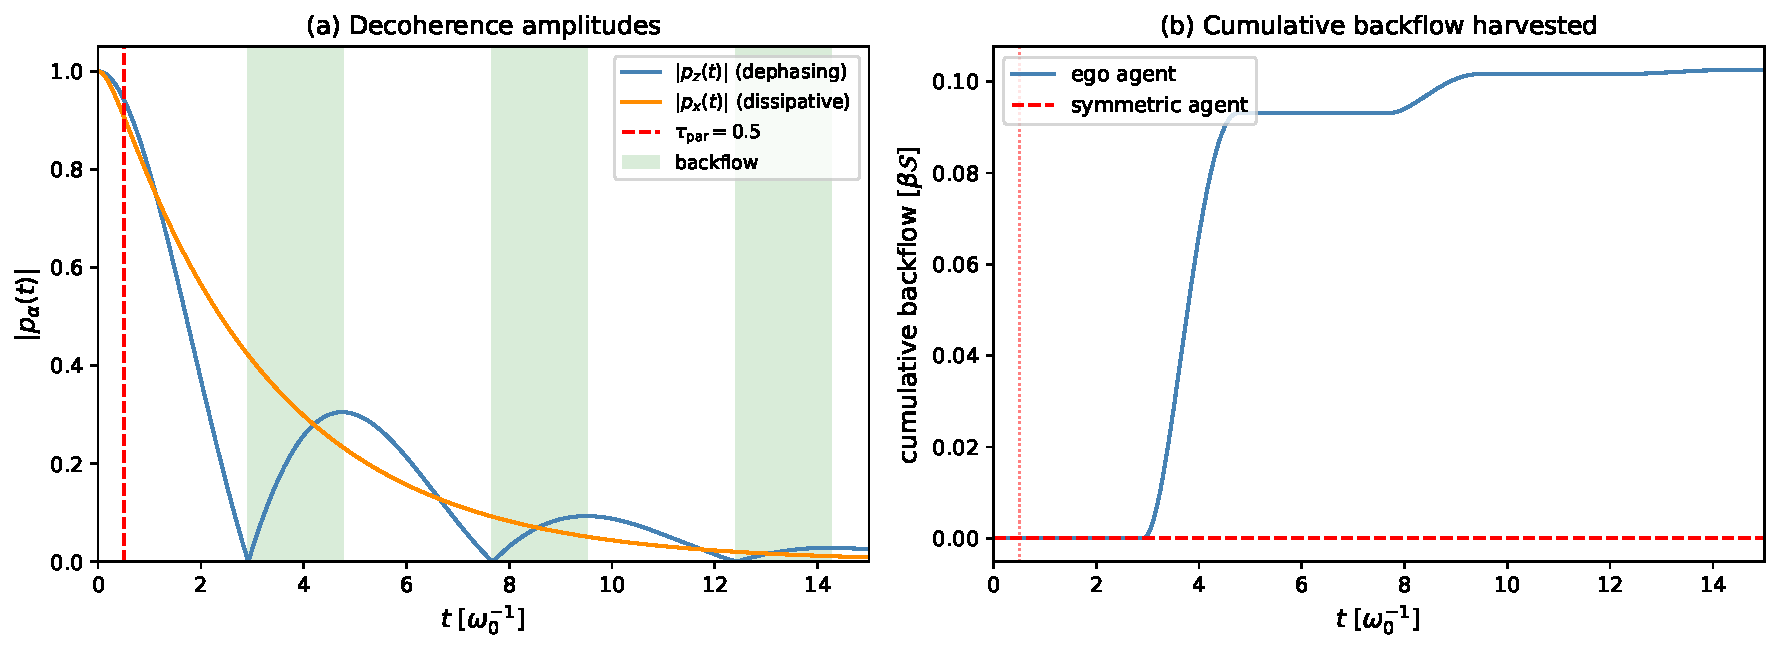
\includegraphics[width=\textwidth]{fig_ego.pdf}
\caption{%
Two-channel qubit model (Section~\ref{II-sec:example}) with
Lorentz--Drude spectral density.
\textbf{Parameters:}
$\omega_0 = 1$ (energy unit);
$\lambda_z = 1$, $\gamma_z = 0.5$ (dephasing, non-Markovian);
$\lambda_x = 0.3$, $\gamma_x = 5.0$ (dissipative,
$\sim$Markovian);
$\mathcal{C}_{\mathrm{budget}} = 2\,h_\mu$.
\textbf{Units:} time in $\omega_0^{-1}$.
\textbf{Regime:} low temperature ($\beta\omega_0 \gg 1$);
using the standard $T \to 0$ analytic
expression~\eqref{II-eq:decoherence_II}~%
\cite{BreuerPetruccione2002}.
\textbf{(a)}~Decoherence amplitudes $|p_z(t)|$ (blue,
non-Markovian, with backflow in green bands) and
$|p_x(t)|$ (orange, monotonic decay).
Red dashed: raw full-sweep depth $\tau_{\max} = 0.5$.
\textbf{(b)}~Cumulative backflow harvested.
Blue: ego agent (broken $\to \sigma_z$) exploits all three
revival intervals.
Red dashed: the stipulated raw full-sweep agent stops at
$\tau_{\max}$; all plotted backflow occurs later.
The growing gap is the \emph{ego dividend}.}
\label{II-fig:ego}
\end{figure}

\paragraph{Accounting check.}
The raw update load is $h_\mu D=4h_\mu$ while the budget is
$2h_\mu$, so that declared representation does not fit.  The example
then \emph{chooses} the two-component dephasing frame ($k^*=2$); for
that choice,
$R_{\mathcal{F}} = 2\,h_\mu
= \mathcal{C}_{\mathrm{budget}}$.  Saturation is an example property,
not a general consequence of monotonic distortion.

% ------------------------------------------------------------
\subsection{The Pointer-State Connection}
\label{II-subsec:pointer}

In this example the chosen basis coincides with an einselection
(environment-induced superselection) basis of the dephasing
model~\cite{Zurek2009}.
The coordinate optimization can select pointer-aligned components when
the declared distortion assigns them the highest survival value per
bit.  This alignment is verified only within a concrete model and is not
generic rate-distortion theorem.

\begin{remark}[Decoherence as symmetry-breaking catalyst]
\label{II-rem:decoherence}
The environment does not \emph{force} a specific gauge fixing.  A
pointer-aligned frame is selected only if the declared distortion and
encoder class rank it above the alternatives.  The present example
chooses that ranking; it does not derive it from bounded computation.
\end{remark}

% ============================================================
\section{The Cost of Ego}
\label{II-sec:cost}

Coordinate selection reduces the declared raw load but can introduce a
blind subspace. A fixed reference frame is a \emph{static}
gauge choice in a \emph{dynamic} environment.
If the environment changes, the ego becomes progressively
maladaptive.

\paragraph{Drift layer.}
Environmental change can occur at multiple levels:
parameter drift ($\lambda_\alpha(t)$, $\gamma_\alpha(t)$),
spectral-density deformation ($J(\omega, t)$), or
full process-distribution shift ($P_t(X)$).
For analytical tractability, we model drift at the
\emph{spectral-density parameter level} throughout this
section.  No monotone extension to arbitrary distribution shift is
claimed.

% ------------------------------------------------------------
\subsection{The Rigidity Trap}
\label{II-subsec:rigidity}

\begin{proposition}[Frame Rigidity under Drift]
\label{II-prop:rigidity}
Let the environment undergo slow drift: the spectral density
parameters change as
$\lambda_\alpha(t) = \lambda_\alpha^{(0)}
+ \varepsilon\,f_\alpha(t)$
for $\alpha \in \{z, x\}$, with drift rate
$\varepsilon > 0$.
Assume the supplied distortion has a locally unique $C^1$
minimizer $\mathcal{F}^*(\lambda)\in G$ and
$\lVert D_\lambda\mathcal F^*\rVert\leq K$ along the path.

If the agent's reference frame $\mathcal{F}$ is held fixed
(no recalibration), the mismatch between $\mathcal{F}$
and $\mathcal{F}^*(t)$ then obeys
\begin{equation}
\label{II-eq:mismatch}
\delta(t)
:= d_G\bigl(\mathcal{F},\, \mathcal{F}^*(t)\bigr)
\leq K\varepsilon \int_0^t \lVert\dot{f}(s)\rVert\,ds,
\end{equation}
where $d_G$ is the geodesic distance in the gauge group.
\end{proposition}

\begin{proof}
The chain rule and the stated sensitivity bound give
$\lVert\dot{\mathcal F}^*(t)\rVert
\leq K\varepsilon\lVert\dot f(t)\rVert$.
Integrating path length bounds the geodesic distance and yields
\eqref{II-eq:mismatch}.
\end{proof}

% ------------------------------------------------------------
\subsection{Stylized Drift Model}
\label{II-subsec:drift_model}

To quantify the loss of visibility of a fixed frame, we use the linear
drift supported by Proposition~\ref{II-prop:rigidity}.  No unstable
environmental dynamics or Lyapunov exponent is assumed.

\begin{definition}[Rotating optimal frame]
\label{II-def:drift}
Let the mismatch angle $\theta(t)$ between the agent's
fixed frame $\mathcal{F}$ and the instantaneous optimal
frame $\mathcal{F}^*(t)$ evolve as
\begin{equation}
\label{II-eq:theta}
\theta(t) = \theta_0+\varepsilon t,
\end{equation}
where $\theta_0 \in (0, \pi/4)$ is the initial misalignment
(so that the crossover time below is positive) and
$\varepsilon>0$ is the angular drift rate.  This is a local model up to
the first visibility crossover, not a claim about long-time motion on
the compact gauge group.

The visible and hidden survival components decompose
geometrically:
\begin{equation}
\label{II-eq:vis_hid_theta}
\mathcal{S}_{\mathrm{vis}}(t)
= \mathcal{S}_{\mathrm{tot}}\,\cos^2\theta(t),
\qquad
\mathcal{S}_{\mathrm{hid}}(t)
= \mathcal{S}_{\mathrm{tot}}\,\sin^2\theta(t),
\end{equation}
where $\mathcal{S}_{\mathrm{tot}}$ is the full survival
functional (invariant under frame rotation).
\end{definition}

% ------------------------------------------------------------
\subsection{The Prediction Error Divergence}
\label{II-subsec:divergence}

\begin{proposition}[Growth of the hidden component]
\label{II-prop:divergence}
Under the drift model~\eqref{II-eq:theta}--\eqref{II-eq:vis_hid_theta},
the hidden survival component grows as
\begin{equation}
\label{II-eq:divergence}
\bigl|\mathcal{S}_{\mathrm{hid}}(t)\bigr|
= |\mathcal{S}_{\mathrm{tot}}|\,\sin^2\!\bigl(\theta_0+
  \varepsilon t\bigr).
\end{equation}
For small angles ($\theta_0+\varepsilon t \ll 1$):
$|\mathcal{S}_{\mathrm{hid}}| \approx
|\mathcal{S}_{\mathrm{tot}}|(\theta_0+\varepsilon t)^2$.
\end{proposition}

\begin{proof}
Direct substitution of~\eqref{II-eq:theta}
into~\eqref{II-eq:vis_hid_theta}.
The small-angle expansion $\sin^2\theta\approx\theta^2$ gives the
quadratic form.
\end{proof}

% ------------------------------------------------------------
\subsection{Visibility Crossover and Conditional Gradient Reversal}
\label{II-subsec:delusion}

\begin{proposition}[Visibility crossover and a conditional gradient reversal]
\label{II-prop:delusion_model}
Under~\textup{(B1)--(B5)} with the drift
model~\eqref{II-eq:theta} and initial misalignment
$\theta_0 \in (0,\,\pi/4)$, an agent with a fixed
reference frame $\mathcal{F}$ reaches the visibility crossover
\begin{equation}
\label{II-eq:t_delusion}
t_{\mathrm{vis}}
= \frac{\pi/4-\theta_0}{\varepsilon},
\end{equation}
at which the hidden and visible magnitudes are equal.  For
$t>t_{\mathrm{vis}}$, the hidden magnitude is larger while
$\theta(t)<\pi/2$.  This geometric crossover alone implies neither
gradient anti-correlation nor failure of every in-frame detector.

There nevertheless exist specified controllers for which gradients do
reverse.  In the two-mode model
\begin{equation}
\label{II-eq:two_mode_losses}
\mathcal S_{\mathrm{vis}}(u)=-\tfrac12(u-1)^2,
\qquad
\mathcal S_{\mathrm{full}}(u,\theta)
=-\tfrac12\lVert u e_1-y^*(\theta)\rVert^2,
\quad
y^*(\theta)=\cos\theta\,e_1+\sin\theta\,e_2,
\end{equation}
the two scalar update directions are anti-correlated exactly when
\begin{enumerate}
\item[] $\cos\theta(t)<u<1$.
\end{enumerate}
Thus the reversal time is controller- and state-dependent; it need not
coincide with $t_{\mathrm{vis}}$.
\end{proposition}

\begin{proof}
The crossover $|\mathcal{S}_{\mathrm{hid}}|
= |\mathcal{S}_{\mathrm{vis}}|$ occurs when
$\sin^2\theta = \cos^2\theta$, i.e.,
$\theta(t_{\mathrm{vis}}) = \pi/4$.
Substituting~\eqref{II-eq:theta}:
$\theta_0+\varepsilon t_{\mathrm{vis}} = \pi/4$,
which gives~\eqref{II-eq:t_delusion}.
For~\eqref{II-eq:two_mode_losses},
$\partial_u\mathcal S_{\mathrm{vis}}=1-u$ and
$\partial_u\mathcal S_{\mathrm{full}}=\cos\theta-u$.
Their product is negative exactly when $u$ lies strictly between
$\cos\theta$ and $1$.  Outside that interval the two gradients agree
in sign or one vanishes.  The calculation exhibits the claimed effect
without promoting it to a universal consequence of visibility loss.
\end{proof}

\begin{remark}[Model scope]
\label{II-rem:linear_drift}
For $\theta_0=0$, the crossover occurs at
$t_{\mathrm{vis}} = \pi/(4\varepsilon)$.
With $\varepsilon = 0.01\,\omega_0$,
$t_{\mathrm{vis}} \approx 79\,\omega_0^{-1}$---long
enough for the agent to accumulate a false sense of
security, yet short on environmental timescales.
Neither this number nor the two-mode sign condition proves that an
agent cannot detect drift from residual statistics; Paper~III studies
one such detector.
\end{remark}

\begin{remark}[Why dithering does not help]
\label{II-rem:dithering}
One might ask whether the agent could escape the delusion
trap by randomly ``probing'' the background subspace
$V_{\mathrm{bg}}$---temporarily rotating its frame to
sample hidden components.
In the raw-coordinate model, a full probe competes with foreground
processing at the component-count rate in
Remark~\ref{II-rem:symmetry_tax}.  This does not prove dithering fails:
randomized exploration can reveal hidden directions, with a
model-dependent cost--benefit trade-off.  A deterministic in-frame
controller may lack a signal indicating when or where to probe.
As long as $|\mathcal{S}_{\mathrm{hid}}|
< |\mathcal{S}_{\mathrm{vis}}|$ (pre-delusion), the
in-frame performance metric $\mathcal{S}_{\mathrm{vis}}$
shows no anomaly.
The linear-drift visibility model below motivates monitoring residual
statistics, the subject of Paper~III, but does not rule out other
exploration policies.
\end{remark}

\begin{remark}[The ego as medicine and poison]
\label{II-rem:medicine_poison}
In this model, coordinate selection reduces raw load but creates a blind
subspace.  The visibility crossover below motivates Paper~III.  This is
a conditional engineering trade-off, not an irreversible logic chain.
\end{remark}

% ------------------------------------------------------------
\subsection{The Origin of Paper~III}
\label{II-subsec:paper3}

To respond to the visibility loss in this model, the agent may use a mechanism
to monitor the quality of its own reference frame---to
``observe its own observation.''
This requires a \emph{second-order control loop}: a
meta-controller that adjusts the gauge fixing $\sigma$ in
response to accumulated prediction errors.

The distribution of in-frame prediction residuals can itself change as
the frame becomes stale.  Paper~III studies whether a specified
likelihood model makes that change statistically identifiable.  This
paper does not prove that Fisher information is the unique detector or
that every controller must add such a loop.

This is the subject of Paper~III: the Fisher information
geometry of self-referential calibration, and the
thermodynamic cost of the loop that closes the chain
\emph{Chaos $\to$ Time $\to$ Self $\to$ Calibration}.

% ============================================================
\section{Numerical Demonstration}
\label{II-sec:numerical}

The preceding sections establish analytic bounds and a
worked example with a qubit in a two-channel bath.
We now compare budgeted coordinate-selection rules in a minimal
multi-dimensional system.  The observed attention concentration and
selection advantage are properties of this supplied algorithm and
environment.
Full code and parameters are provided for reproducibility.

% ------------------------------------------------------------
\subsection{Model}
\label{II-subsec:demo_model}

\paragraph{Environment.}
A $D$-dimensional linear prediction task with sparse
rotating support:
$y(t) = \mathbf{w}^*(t)^\top \mathbf{x}(t) + \xi(t)$,
$\mathbf{x}(t) \sim \mathcal{N}(\mathbf{0}, \mathbf{I}_D)$,
$\xi \sim \mathcal{N}(0, \sigma^2)$.
Only $m \ll D$ dimensions carry nonzero weight at any time;
the active support rotates every $\tau_{\mathrm{switch}}$
steps, modelling environmental drift.

\paragraph{Hard budget constraint.}
Per step, the agent may update only $k$ coordinates of its
weight vector (a hard processing budget), mirroring the
bounded computation assumption~(B2).

\paragraph{Agents.}
\begin{itemize}
\item \textbf{Budgeted selector}: selects the top-$k$
  dimensions by importance score---an exponential moving
  average of the signed per-coordinate gradient.  Signed
  accumulation ensures that noise dimensions (zero expected
  signal) cancel over time while signal dimensions persist,
  enabling reliable discrimination without access to the true
  support.
\item \textbf{Random-$k$ baseline}: selects $k$ dimensions
  uniformly at random each step.  This provides a
  budget-fair comparison with no persistent coordinate preference.
\end{itemize}

\noindent
The choice of \emph{signed} gradient EMA (rather than
squared-gradient magnitude) is structurally motivated:
for noise dimensions $\mathbb{E}[r\,x_i] = 0$, so the
signed accumulation cancels over time; for signal
dimensions $\mathbb{E}[r\,x_i] \neq 0$, so a consistent
directional bias persists.  The signed EMA thus acts as a
\emph{directional coherence filter} that discriminates
signal from noise without access to the true support---a
minimal model of a persistent coordinate preference.

\paragraph{Parameters.}
\begin{center}
\small
\begin{tabular}{@{}lcl@{}}
\toprule
\textbf{Quantity} & \textbf{Value} & \textbf{Role} \\
\midrule
$D$ & 64 & ambient dimension \\
$m$ & 8  & signal dimensions (sparse support) \\
$T$ & $10{,}000$ & horizon per trial \\
Seeds & 10 & independent replications \\
$\sigma$ & 0.3 & observation noise std \\
$\eta$ & 0.02 & SGD learning rate \\
$\lambda$ & 0.995 & weight decay per step \\
$k$ & 2, 4, 6, 8, 10, 12, 16, 20, 24, 32, 48, 64
  & budget grid \\
$\tau_{\mathrm{switch}}$ & $\{500, 1000, 2000\}$
  & support rotation period \\
\bottomrule
\end{tabular}
\end{center}

\paragraph{Attention entropy.}
Let $n_i$ be the number of updates coordinate $i$ receives
in a measurement window of the last $1{,}000$ steps.
The normalised update frequency
$p_i = n_i / \sum_j n_j$ defines the attention entropy:
\begin{equation}
\label{II-eq:H_attn}
H_{\mathrm{attn}} = -\sum_{i=1}^{D} p_i \ln p_i.
\end{equation}
Under uniform coordinate selection, $p_i = 1/D$ and
$H_{\mathrm{attn}} = \ln D$.  Under budget-constrained
selection, $H_{\mathrm{attn}}$ collapses away from $\ln D$,
measuring concentration of the update rule.  It is not by itself a
thermodynamic order parameter.

\paragraph{Oracle metric.}
Neither agent has access to $\mathbf{w}^*(t)$.
Performance is evaluated externally using the
weight-space mean-squared error
$\mathrm{MSE} = \|\hat{\mathbf{w}} - \mathbf{w}^*\|^2$,
averaged over post-burn-in steps.

% ------------------------------------------------------------
\subsection{Results}
\label{II-subsec:demo_results}

Figure~\ref{II-fig:kstar_scaling} shows the two key signatures.

\paragraph{Result 1: Attention entropy collapse
(Figure~\ref{II-fig:kstar_scaling}a).}
Under fixed support (no rotation), the attention entropy
$H_{\mathrm{attn}}$ exhibits a sharp collapse away from
$\ln D = \ln 64 \approx 4.16$ and increases monotonically
with $k$, consistent with a budget-induced concentration
of update mass onto signal-carrying dimensions.
For budgets near and below the signal scale ($k \leq m$),
$H_{\mathrm{attn}}$ remains $O(\ln m)$, consistent with
confinement to the signal subspace.
We use the collapse of $H_{\mathrm{attn}}$ away from
$\ln D$ as the order parameter of symmetry breaking;
a strict plateau at $\ln m$ is not expected under the
present re-selection dynamics and finite-window estimator.

\paragraph{Result 2: Selection advantage
(Figure~\ref{II-fig:kstar_scaling}b).}
Under rotating support, the mean-squared error gap
$\Delta\mathrm{MSE} = \mathrm{MSE}_{\mathrm{rnd}}
- \mathrm{MSE}_{\mathrm{sel}}$ is positive for
$k \lesssim 3m$ and peaks at tight budgets ($k = 2$)
where the selection advantage is strongest.
For $k \gg m$ the gap turns slightly negative
(the selector's commitment to stale dimensions costs
more than the random baseline's diversification),
before returning to zero at $k = D$.
The three $\tau_{\mathrm{switch}}$ curves are ordered:
slower drift (larger $\tau$) yields a larger peak gap,
with the ordering most visible at small $k$.

\begin{figure}[t]
\centering
\includegraphics[width=\textwidth]%
  {fig_paper2_kstar_scaling.pdf}
\caption{%
\textbf{Budgeted coordinate selection in the declared linear model.}
$D = 64$, $m = 8$, $T = 10{,}000$, 10 seeds, 95\% CI bands.
\textbf{(a)}~Attention entropy $H_{\mathrm{attn}}$ vs
budget $k$ (fixed support).  The empirical curve (blue)
collapses from $\ln D \approx 4.16$ toward an
$O(\ln m)$ floor as budget tightens.
For $k \leq m$, $H_{\mathrm{attn}}$ remains below
$\ln m \approx 2.08$ (green dashed), consistent with
confinement to the signal subspace.
\textbf{(b)}~Selection advantage
$\Delta\mathrm{MSE} = \mathrm{MSE}_{\mathrm{rnd}}
- \mathrm{MSE}_{\mathrm{sel}}$ vs budget $k$ under
rotating support.  The gap is positive for $k \lesssim 3m$
(selection helps), turns slightly negative at large $k$
(commitment cost exceeds diversification), and returns
to zero at $k = D$.  Slower drift ($\tau = 2000$)
yields a larger peak advantage.}
\label{II-fig:kstar_scaling}
\end{figure}

% ------------------------------------------------------------
\subsection{Scope of This Demonstration}
\label{II-subsec:demo_scope}

These simulations compare two supplied coordinate-selection rules in
the stated sparse linear model.  They do not establish a universal
symmetry-breaking transition or identify the capacity $k_{\max}$ with
an information-bottleneck optimum.

\medskip
This demonstration \textbf{does} show:
\begin{enumerate}
\item Under hard budget constraints, attention entropy
  collapses sharply away from $\ln D$ and remains
  $O(\ln m)$ for $k \leq m$---the agent confines its
  updates to the signal subspace.
  This measures concentration of the chosen update rule.
\item A budgeted selector that exploits importance-weighted
  selection systematically outperforms a budget-fair
  random baseline, consistent with a survival advantage
  for the parameter range shown.
\item The advantage scales with both budget tightness
  (smaller $k$) and environmental stability (larger
  $\tau_{\mathrm{switch}}$).
\end{enumerate}

\noindent
In summary, this demonstration establishes a model-specific selection
advantage and a measurable attention-concentration statistic; it does
not derive selection from the budget or claim universality across
architectures or environment classes.

\medskip
This demonstration does \textbf{not} show:
\begin{enumerate}
\item That $H_{\mathrm{attn}}$ reaches a strict plateau
  at $\ln m$ for all $k \leq m$.  Under the adaptive
  re-selection dynamics used here, the selector cycles
  within the signal subspace, producing
  $H_{\mathrm{attn}}$ values near but not locked to
  $\ln m$.  The relevant signature is the collapse
  \emph{away from} $\ln D$, not convergence to a
  specific lower bound.
\item That the specific form of the importance score
  (signed gradient EMA) is optimal.  It is one
  realisation of the selection mechanism.
\item That the results generalise to all environment
  classes.  The model uses Gaussian features, linear
  regression, and sparse rotating support.
\item That the delusion--correction cycle is addressed.
  This is the subject of Paper~III.
\item That a sharp thermodynamic phase transition occurs, or that
  $k=k_{\max}$ is the distortion-minimizing retained dimension.
\end{enumerate}

\paragraph{Reproducibility.}
\begin{sloppypar}
The complete simulation is a self-contained Python script
(\texttt{paper2\_kstar\_scaling\_demo.py}, ${\sim}\,540$
lines, requiring only NumPy and Matplotlib) with fixed
random seeds.  All figures in this section can be
reproduced by executing the script.  The following files
are included in the supplementary archive:
\begin{itemize}
\item \texttt{paper2\_kstar\_scaling\_demo.py} --- simulation script
\item \texttt{fig\_paper2\_kstar\_scaling.pdf} --- Figure~\ref{II-fig:kstar_scaling}
\item \texttt{kstar\_scaling\_data.csv} --- raw performance gap data
\end{itemize}
\end{sloppypar}

% ============================================================
\section{Discussion}
\label{II-sec:discussion}

% ------------------------------------------------------------
\subsection{Summary of Results}
\label{II-subsec:summary}

\begin{center}
\small
\setlength{\tabcolsep}{4pt}%
\begin{tabular}{@{}lP{6cm}c@{}}
\toprule
\textbf{Result} & \textbf{Statement} & \textbf{Sec.} \\
\midrule
Raw-channel load
  & A declared $D$-channel archive costs $D h_\mu$ per
    incremental update; this is accounting, not a lower bound
  & \ref{II-sec:ceiling} \\[3pt]
Compression existence
  & A minimizer exists in the supplied compact encoder class and has
    $k_{\mathrm{opt}}\leq k_{\max}$
  & \ref{II-subsec:RD_bound} \\[3pt]
Conditional frame selection
  & A chosen proper projection breaks the declared model symmetry when
    no invariant feasible encoder meets the target
  & \ref{II-subsec:SSB} \\[3pt]
Four diagnostics
  & Frame-dependent models can be audited using $\mathcal{B}_{\mathrm{select}}$,
    $\mathcal{B}_{\mathrm{frame}}$,
    $\mathcal{B}_{\mathrm{center}}$,
    $\mathcal{B}_{\mathrm{inc}}$
  & \ref{II-subsec:bias} \\[3pt]
Survival Decomposition
  & $\mathcal{S} = \mathcal{S}_{\mathrm{vis}} +
    \mathcal{S}_{\mathrm{hid}}$
  & \ref{II-subsec:effective} \\[3pt]
Uniform-channel trade-off
  & Predictive loss is approximately $1-k^*/D$ only under the
    uniform raw-channel assumption
  & \ref{II-subsec:tradeoff} \\[3pt]
Visibility crossover
  & Linear drift gives $t_{\mathrm{vis}}=(\pi/4-\theta_0)/\varepsilon$;
    gradient reversal requires a separate controller condition
  & \ref{II-subsec:delusion} \\[3pt]
Numerical demo
  & Attention concentration and model-specific selection advantage
    (Fig.~\ref{II-fig:kstar_scaling})
  & \ref{II-sec:numerical} \\
\bottomrule
\end{tabular}
\end{center}

% ------------------------------------------------------------
\subsection{Testable Predictions}
\label{II-subsec:predictions}

The conditional model claims can be tested without treating them as
universal laws.  First, vary $k$, $D$, and the support-switching time in
the declared sparse linear environment and compare the supplied selector
with random and alternative compressed baselines.  A sharp transition is
not predicted without a separately defined thermodynamic limit.

Second, estimate
$I(X_{\mathrm{past}};X_{\mathrm{future}})$ and
$I(\hat X_{\mathrm{past}};X_{\mathrm{future}})$ while varying $k/D$.
Linear $1-k/D$ scaling tests the uniform-allocation assumption in
Theorem~\ref{II-thm:tradeoff}; systematic curvature falsifies that
assumption rather than information theory.

Third, in a controlled rotating-feature task, measure both the visibility
ratio and the inner product of surrogate and oracle gradients.  The
linear model predicts the visibility crossover at
$t_{\mathrm{vis}}=(\pi/4-\theta_0)/\varepsilon$.  Proposition~\ref{II-prop:delusion_model}
predicts gradient reversal only for controllers entering the region
$\cos\theta(t)<u(t)<1$; coincidence of the two events is not required.

% ------------------------------------------------------------
\subsection{What This Paper Does and Does Not Show}
\label{II-subsec:claims}

This paper \textbf{does} show:
\begin{enumerate}
\item A declared raw $D$-channel archive has the stated component-count
  load, and a minimizer exists in the supplied compact encoder class.
\item A proper coordinate projection privileges a frame; under additional
  feasibility assumptions this can be interpreted as operational symmetry
  breaking (Remark~\ref{II-rem:conditional_ssb}).
\item Definition~\ref{II-def:bias} supplies four model diagnostics, with the
  extra controller and task assumptions needed by each made explicit.
\item Linear frame drift produces a visibility crossover, while the
  two-mode model exhibits a separate, conditional gradient reversal
  (Proposition~\ref{II-prop:delusion_model}).
\item A minimal computational demonstration measures attention
  concentration and a selection advantage over a budget-fair random baseline
  (Section~\ref{II-sec:numerical},
  Figure~\ref{II-fig:kstar_scaling}).
\end{enumerate}

\medskip
This paper does \textbf{not} show:
\begin{enumerate}
\item That bounded computation uniquely determines a privileged basis,
  forces symmetry breaking, or makes the chosen frame survival-optimal.
\item That symmetry breaking is necessary or sufficient for persistence.
\item That the ``ego'' implies or requires consciousness,
  subjective experience, or phenomenal awareness.
  The term is used strictly in the control-theoretic sense.
\item That this framework constitutes a theory of
  consciousness. It is a theory of computational optimality
  under thermodynamic constraints.
\item That the four diagnostics exhaust self-reference or follow from
  gauge fixing alone.
\item That the coordinate capacity is a Shannon rate--distortion bound or
  is achievable by a specific physical implementation.
\item That visibility loss forces gradient reversal or is undetectable.
  Paper~III analyzes one conditional calibration model.
\item That the framework constitutes or implies a
  philosophical or metaphysical claim about the nature
  of selfhood.
\item That this framework applies to all possible physical
  systems. It applies to systems
  satisfying the declared channel, encoder, controller, and drift
  assumptions.
\item That the Clifford algebra is the only possible
  algebraic setting. It is supplied here as a model input; Q-RAIF does
  not uniquely derive it.
\end{enumerate}

% ============================================================
% REFERENCES
% ============================================================

% ============================================================================
% Paper III --- ``The Loop''
% ============================================================================
\chapter{Fisher Information Geometry and Conditional Implementation Costs of Self-Referential Calibration}
\label{chap:paperIII}

\begin{center}
\textit{Paper III --- ``The Loop''}\\[0.5em]
Originally published: Zenodo, DOI: 10.5281/zenodo.18591771
\end{center}

\bigskip

\section*{Abstract}
Papers~I and~II of the T-DOME
series~\cite{Liu2026TDOME_I,Liu2026TDOME_II} supply conditional
resource and reference-frame models for persistent agents.  They do not
prove that all persistent agents require non-Markovian memory or
spontaneous Clifford gauge-symmetry breaking.  Paper~II's linear-drift
visibility crossover is likewise a declared coordinate model, not a
universal logarithmic ``Delusion Trap'' timescale.

This paper studies \textbf{self-referential calibration} under explicit
residual-likelihood, prior, drift, convexity, and hardware assumptions.
The agent uses the score statistics of a supplied prediction-residual
model to estimate frame mismatch.  The principal conditional results are:
\begin{enumerate}
\item \textbf{Gaussian Fisher Signal}
  (Proposition~\ref{III-prop:gaussian_fisher}):
  in the declared even Gaussian residual model, per-sample local Fisher
  information grows quadratically and accumulated information grows
  cubically.  Detection precedes the visibility crossover if and only if
  the threshold condition in Corollary~\ref{III-cor:detection_window} holds.
\item \textbf{Self-Referential Cram\'{e}r--Rao Bound}
  (Theorem~\ref{III-thm:SRCR}):
  the van Trees lower bound applies under the stated regular likelihood,
  conditional-independence, compact-support, and prior assumptions, with
  data and prior Fisher information entering separately.
\item \textbf{Conditional Implementation Cost}
  (Proposition~\ref{III-prop:loop_cost_impl}):
  a separable implementation with declared irreversible sensor and
  computational resets and linear-response actuation obeys
  $\dot{W}_{\mathrm{loop}}
  \geq k_BT\,\ln 2\,(R_s+R_c)
  + \mathcal{L}^2/\tau_{\mathrm{recalib}}^2$,
  a bound for that implementation rather than a universal cost of
  sensing, Fisher evaluation, or self-reference.
\end{enumerate}

The calibration loop has a local tracking bound only under geodesic
strong convexity and bounded drift (Theorem~\ref{III-thm:loop_stability}).
The four supplied layers in Definition~\ref{III-def:four_part_template}
define the running model architecture; they are not proved necessary,
sufficient, minimal, or complete for persistent agency.  ``Reflexivity''
here denotes one implementation of second-order control, with no claim of
architectural uniqueness or phenomenal consciousness.


% ============================================================
\section{Introduction}
\label{III-sec:intro}

% ------------------------------------------------------------
\subsection{Context: The Delusion Trap}
\label{III-subsec:delusion_context}

Revised Paper~II~\cite{Liu2026TDOME_II} studies a supplied
coordinate projection under a raw-channel budget.  It does not prove
that persistence forces Clifford gauge symmetry breaking.  Its drift
model uses a linearly changing mismatch
$\theta(t)=\theta_0+\varepsilon t$ and identifies the geometric
visibility crossover
\begin{equation}
\label{III-eq:t_del_recall}
t_{\mathrm{vis}}
=\frac{\pi/4-\theta_0}{\varepsilon}.
\end{equation}
That crossover does not by itself imply gradient reversal or
undetectability.  The present paper asks a narrower question: for a
specified residual likelihood, can score statistics detect mismatch,
and under what conditions can a natural-gradient controller track a
moving optimum?

% ------------------------------------------------------------
\subsection{Position within Papers~I--III}
\label{III-subsec:sequence}

This paper is the third and final of the T-DOME framework,
closing the three-paper sequence.

\begin{center}
\small
\setlength{\tabcolsep}{4pt}%
\begin{tabular}{@{}lP{3.5cm}P{4.2cm}c@{}}
\toprule
\textbf{Framework} & \textbf{Question} & \textbf{Result}
  & \textbf{Status} \\
\midrule
HAFF~\cite{Liu2026HAFF_A,Liu2026HAFF_B}
  & How does geometry emerge?
  & Conditional algebra/dictionary models
  & Revised \\[3pt]
Q-RAIF~\cite{Liu2026QRAIF_A,Liu2026QRAIF_B}
  & What algebra must an observer have?
  & Clifford representations as model inputs
  & Revised \\[3pt]
T-DOME~I~\cite{Liu2026TDOME_I}
  & What can inter-epoch correlations fund?
  & Restricted baseline; correlation accounting
  & Conditional \\[3pt]
T-DOME~II~\cite{Liu2026TDOME_II}
  & When can a model select a frame?
  & Conditional coordinate selection
  & Conditional \\[3pt]
\textbf{T-DOME~III} (this work)
  & How does self-calibration arise?
  & Fisher self-referential bound;
    thermodynamic cost of reflexivity
  & \textbf{This paper} \\
\bottomrule
\end{tabular}
\end{center}

The three T-DOME papers form a conditional modelling sequence:
\begin{enumerate}
\item \textbf{Paper~I:} Initial correlations can enter an ELV-type
  thermodynamic balance; a restricted autonomous baseline is proved.
\item \textbf{Paper~II:} A raw-coordinate archive motivates a supplied
  compression model and a linear visibility-crossover example.
\item \textbf{Paper~III (this work):} Uncorrected
  bias diverges from a changing environment.
  A self-referential calibration loop---monitoring the
  Fisher information of one's own prediction stream---resolves
  mismatch under explicit likelihood and convexity assumptions.  A
  conditional hardware model assigns reset and actuation costs.
\end{enumerate}

The links are motivation and model interfaces, not an irreversible
theorem chain.  None of the three papers proves that this architecture
is necessary for persistence.

% ------------------------------------------------------------
\subsection{The Information-Geometric Insight}
\label{III-subsec:insight}

The key observation that resolves the Delusion Trap is
subtle:
\emph{while the agent cannot observe $V_{\mathrm{bg}}$
directly, it can observe the statistical properties of its
own prediction residuals in $V_{\mathrm{fg}}$.}

The prediction residual
$e(t) := \mathcal{S}_{\mathrm{vis}}(t)
- \mathcal{S}_{\mathrm{vis}}^{(\mathrm{pred})}(t)$
lies in $V_{\mathrm{fg}}$ by construction.
In the declared even Gaussian model, a record cannot identify the sign
of mismatch.  Its \emph{distribution}---the probability law
$p(e\,|\,\sigma)$, parametrised by the gauge-fixing
parameter~$\sigma$---does depend on~$\sigma$, because the
projection $\Pi_{\mathcal{F}}(\sigma)$ determines which
environmental correlations are captured and which are
discarded.

When the frame $\sigma$ drifts away from the optimal
$\sigma^*$, the residual distribution shifts.
The \emph{Fisher information metric}
\begin{equation}
\label{III-eq:fisher_preview}
g_{ij}(\sigma)
= \mathbb{E}_\sigma\!\left[
  \frac{\partial \log p(e\,|\,\sigma)}
       {\partial \sigma^i}\,
  \frac{\partial \log p(e\,|\,\sigma)}
       {\partial \sigma^j}
\right]
\end{equation}
measures the sensitivity of this distribution to changes
in~$\sigma$.
Whether $g_{ij}$ changes with staleness is likelihood-dependent.  The
Gaussian model below provides one explicit case.

This is the mathematical realisation of the
``second-order operation'' demanded by
Paper~II, Section~7.5: the agent does not need to see the
truth (the full $Cl(V,q)$), but only the \emph{rate of
change of its own prediction error} as a function of its
frame parameters.
Fisher information is one local sensitivity measure, not the unique
possible detector.

% ------------------------------------------------------------
\subsection{Relation to Architectural Incompleteness}
\label{III-subsec:haff_g}

Revised HAFF Paper~G~\cite{Liu2026HAFF_G} supplies
philosophy-of-science motivation rather than a fixed-point no-go
theorem.  In that motivational sense,
the self-referential calibration loop cannot \emph{eliminate}
architectural incompleteness, but it can \emph{track}
the consequences of incompleteness in real time.
The Lyapunov function $V(\sigma)$ monitors the distance
between the agent's frame and the optimal frame without
requiring access to the ``complete'' description---it
operates entirely within the agent's own predictive
statistics.

% ------------------------------------------------------------
\subsection{Scope and Disclaimers}
\label{III-subsec:scope}

\begin{enumerate}
\item \emph{Reflexivity} refers throughout to
  second-order control: the ability of a system to
  monitor and adjust its own monitoring process.
  It carries \emph{no} implication of phenomenal
  consciousness, subjective experience, or qualia.
\item The self-referential calibration loop does not
  \emph{eliminate} the ego's bias; it tracks and
  compensates for drift in the bias.
  The four bias terms of Paper~II persist in the
  calibrated phase.
\item The thermodynamic cost statement is conditional on irreversible
  reset, separable hardware, and a linear-response actuation model.
\item The framework applies to systems
  satisfying~(C1)--(C5) (Section~\ref{III-subsec:standing_C}).
  It is not a universal theory of agency.
\end{enumerate}

\paragraph{Related work.}
The Fisher information metric on statistical manifolds was
introduced by Rao~\cite{Rao1945} and shown to be unique
by \v{C}encov~\cite{Cencov1982}.
The natural gradient and information geometry were developed
by Amari~\cite{Amari1998,AmariNagaoka2000}.
Thermodynamic length and optimal finite-time transformations
were established by
Crooks~\cite{Crooks2007} and
Sivak--Crooks~\cite{SivakCrooks2012}.
The connection between Fisher information and entropy
production was formalised by Ito~\cite{Ito2018} and
Barato--Seifert~\cite{BaratoSeifert2015}.
Second-order cybernetics originates with
Ashby~\cite{Ashby1956} and
von Foerster~\cite{vonFoerster2003}.
Adaptive control and self-tuning regulators are treated
in~\cite{AstromWittenmark1995}.
The Bayesian Cram\'{e}r--Rao bound (van Trees inequality)
is from~\cite{vanTrees1968}.

\paragraph{Summary of contributions.}
This paper separates three levels of result:
\begin{enumerate}
\item \textbf{Drift Detectability}
  (Proposition~\ref{III-prop:gaussian_fisher}): an explicit Gaussian
  residual likelihood has quadratic per-sample and cubic accumulated
  local Fisher signals; early detection is a threshold condition.
\item \textbf{Self-Referential Cram\'{e}r--Rao Bound}
  (Theorem~\ref{III-thm:SRCR}):
  drift-estimation precision is bounded by the sum of
  data Fisher information and ego rigidity.
\item \textbf{Thermodynamic Cost}
  (Proposition~\ref{III-prop:loop_cost_impl}): a separable implementation
  with irreversible resets and finite-time actuation obeys a conditional
  additive bound.
\end{enumerate}

\paragraph{Result-status ledger.}
The original drift-detectability theorem
\texttt{TD-III-T3.3} is retracted;
Proposition~\ref{III-prop:gaussian_fisher} is an FD/I model calculation and
Corollary~\ref{III-cor:detection_window} is conditional on a declared
threshold.  Ego rigidity \texttt{TD-III-ego} remains a supplied prior
model.  The tracking theorem is conditional on local geodesic strong
convexity.  The universal additive-cost claim
\texttt{TD-III-T6.2} is downgraded to
Proposition~\ref{III-prop:loop_cost_impl}, and the inherited persistence
budget is withdrawn.

% ============================================================
\section{Mathematical Preliminaries}
\label{III-sec:prelim}

% ------------------------------------------------------------
\subsection{Inherited Framework from Papers~I and~II}
\label{III-subsec:inherited}

We briefly recall the key objects; the reader is referred to
Papers~I and~II for full definitions and proofs.

\paragraph{From Paper~I~\cite{Liu2026TDOME_I}.}
\begin{itemize}
\item \textbf{Survival functional.}
  $\mathcal{S}[\Lambda,\tau]
  := \Delta F - W[0,\tau]$~(Paper~I,
  Eq.~(9)).
\item \textbf{Restricted autonomous baseline.}
  $\mathcal{S}[\Lambda^{\mathrm{D}},\tau]\leq0$ for a fixed-Hamiltonian,
  no-control Davies semigroup under its stated initial conditions.  It
  is not a ceiling for all Markovian agents.
\item \textbf{Memory kernel.}
  $\mathcal{K}(t,s)$: the non-Markovian superoperator
  encoding system--environment correlations.
\item \textbf{Entropy rate.}
  $h_\mu := \lim_{T\to\infty}T^{-1}H(X_{0:T})$ (bits per
  unit time per algebraic component).
\item \textbf{Predictive information.}
  $I_{\mathrm{pred}}
  := I(\overleftarrow{X};\,\overrightarrow{X})$.
\end{itemize}

\paragraph{From Paper~II~\cite{Liu2026TDOME_II}.}
\begin{itemize}
\item \textbf{Internal algebra.}
  $\mathcal{O}_{\mathrm{int}} = Cl(V,q)$, $D = \dim Cl(V,q) = 2^n$,
  gauge group $G = \mathrm{Aut}(Cl(V,q))$.
\item \textbf{Gauge bundle.}
  $\pi: P \to M$, structure group $G$; a section
  $\sigma: M \to P$ is a reference frame.
\item \textbf{Ego.}
  $\mathfrak{E} := (\mathcal{F}^*,\,V_{\mathrm{fg}}^*)$
  denotes a chosen optimizer in a supplied encoder class, with
  $k^*=k_{\mathrm{opt}}\leq k_{\max}$.  The budget capacity is not a
  universal optimizer formula.
\item \textbf{Projected kernel.}
  $\mathcal{K}_{\mathcal{F}}(t,s)
  = \Pi_{\mathcal{F}}\,\mathcal{K}(t,s)\,
  \Pi_{\mathcal{F}}$.
\item \textbf{Survival decomposition.}
  $\mathcal{S} = \mathcal{S}_{\mathrm{vis}}(\mathcal{F})
  + \mathcal{S}_{\mathrm{hid}}(\mathcal{F})$.
\item \textbf{Four bias terms.}
  $\mathcal{B}_{\mathrm{select}}$,
  $\mathcal{B}_{\mathrm{frame}}$,
  $\mathcal{B}_{\mathrm{center}}$,
  $\mathcal{B}_{\mathrm{inc}}$
  (revised Paper~II, four-diagnostics definition).  These are model
  diagnostics, not generic consequences of gauge fixing.
\item \textbf{Visibility crossover.}
  $t_{\mathrm{vis}}=(\pi/4-\theta_0)/\varepsilon$ in the supplied
  linear drift geometry.  Gradient reversal requires an additional
  controller condition.
\item \textbf{Information objects.}
  Mutual information is evaluated on explicitly induced record
  processes; algebra symbols are not themselves random variables.
\end{itemize}

% ------------------------------------------------------------
\subsection{Fisher Information Metric}
\label{III-subsec:fisher}

\begin{definition}[Fisher information matrix]
\label{III-def:fisher}
Let $\{p(x\,|\,\theta) : \theta \in \Theta
\subset \mathbb{R}^d\}$ be a parametric family of
probability densities satisfying standard regularity
conditions (interchange of differentiation and integration).
The \emph{Fisher information matrix} is
\begin{equation}
\label{III-eq:fisher_def}
g_{ij}(\theta)
:= \mathbb{E}_\theta\!\left[
  \frac{\partial \log p(x\,|\,\theta)}
       {\partial \theta^i}\,
  \frac{\partial \log p(x\,|\,\theta)}
       {\partial \theta^j}
\right]
= -\mathbb{E}_\theta\!\left[
  \frac{\partial^2 \log p(x\,|\,\theta)}
       {\partial \theta^i\,\partial \theta^j}
\right].
\end{equation}
The pair $(\Theta,\,g)$ is a Riemannian manifold called the
\emph{statistical manifold}.
\end{definition}

\begin{remark}[Uniqueness]
\label{III-rem:cencov}
By \v{C}encov's theorem~\cite{Cencov1982}, the Fisher--Rao
metric $g^{\mathrm{FR}}$ is, up to a positive scalar
multiple, the unique Riemannian metric on the space of
probability distributions that is invariant under all
Markov morphisms (sufficient-statistic embeddings).
Within the hypotheses and category used by \v{C}encov's theorem, this
makes the Fisher metric a canonical local distinguishability metric.
It does not make a Fisher-based detector physically mandatory, nor does
it choose a likelihood or control objective for the agent.
\end{remark}

\begin{proposition}[Cram\'{e}r--Rao bound]
\label{III-prop:CR}
For any unbiased estimator $\hat{\theta}$ of $\theta$ based
on $n$ independent observations:
\begin{equation}
\label{III-eq:CR}
\mathrm{Cov}(\hat{\theta})
\;\succeq\; \frac{1}{n}\,\bigl[g(\theta)\bigr]^{-1}
\end{equation}
in the L\"{o}wner order.
The scalar case reads
$\mathrm{Var}(\hat{\theta})
\geq 1/\bigl(n\,g(\theta)\bigr)$.
\end{proposition}

\begin{remark}[Effective independence]
\label{III-rem:effective_independence}
Throughout this paper, references to ``independent
observations'' in the context of continuous-time residual
streams should be read as \emph{effective independence}
after thinning by the environmental decorrelation
time~$\tau_E$, yielding an effective sample size
$n_{\mathrm{eff}} \approx T/\tau_E$.
In particular, the sample count $n$ in~\eqref{III-eq:CR}
becomes $n_{\mathrm{eff}}$ in the self-referential
setting of Section~\ref{III-subsec:SRCR}.
\end{remark}

\begin{remark}[Fisher metric and KL divergence]
\label{III-rem:fisher_KL}
The Fisher metric arises as the Hessian of the
Kullback--Leibler divergence~\cite{CoverThomas2006}:
\begin{equation}
\label{III-eq:fisher_KL}
D_{\mathrm{KL}}\bigl(p_\theta \,\|\, p_{\theta+d\theta}\bigr)
= \tfrac{1}{2}\,g_{ij}(\theta)\,d\theta^i\,d\theta^j
  + O\!\left(|d\theta|^3\right).
\end{equation}
This identifies the Fisher metric as the infinitesimal
measure of statistical distinguishability.
\end{remark}

% ------------------------------------------------------------
\subsection{Information Geometry}
\label{III-subsec:info_geom}

Following Amari~\cite{Amari1985,AmariNagaoka2000}, the
statistical manifold $(\Theta,\,g)$ carries additional
geometric structure beyond the Riemannian metric.

\paragraph{$\alpha$-connections.}
For each $\alpha \in [-1,\,1]$, Amari defines an affine
connection $\nabla^{(\alpha)}$ on $\Theta$.
The cases $\alpha = 1$ (exponential connection,
$\nabla^{(e)}$) and $\alpha = -1$ (mixture connection,
$\nabla^{(m)}$) are \emph{dual} with respect to $g$:
$\partial_k\,g(X,Y)
= g(\nabla_k^{(e)}X,\,Y)
+ g(X,\,\nabla_k^{(m)}Y)$.
For exponential families, $\nabla^{(e)}$ is flat in natural
parameters and $\nabla^{(m)}$ is flat in expectation
parameters---the \emph{dually flat structure}.
The case $\alpha = 0$ recovers the Levi-Civita connection of
the Fisher metric.

\paragraph{Natural gradient.}
Standard gradient descent in parameter space ignores the
curvature of the statistical manifold.
The \emph{natural gradient}~\cite{Amari1998}
\begin{equation}
\label{III-eq:natural_gradient}
\dot{\theta}
= -\eta\,g^{-1}(\theta)\,\nabla_\theta L(\theta),
\end{equation}
where $\eta > 0$ is the learning rate and $L(\theta)$ is a
loss function, provides the steepest descent direction in the
Fisher metric.
It is reparametrisation-invariant.  Statistical efficiency requires
additional estimator and asymptotic assumptions and is not implied by
the update formula alone.

\paragraph{Pythagorean theorem.}
In a dually flat space, the KL divergence satisfies
a generalised Pythagorean relation:
$D_{\mathrm{KL}}(p\,\|\,r)
= D_{\mathrm{KL}}(p\,\|\,q)
+ D_{\mathrm{KL}}(q\,\|\,r)$
when $q$ is the $m$-projection of $p$ onto a
submanifold containing $r$.
This decomposition will be applied to separate the
foreground-recoverable and background-irrecoverable
components of drift.

% ------------------------------------------------------------
\subsection{Thermodynamic Length}
\label{III-subsec:thermo_length}

\begin{definition}[Thermodynamic length]
\label{III-def:thermo_length}
Let $\lambda(t)$ for $t \in [0,\tau]$ be a path through
control parameter space, and let $\zeta_{ij}(\lambda)$ be the
\emph{friction tensor} (the time-integrated equilibrium
force--force correlation function at~$\lambda$).
The \emph{thermodynamic length} of the
path~\cite{Crooks2007} is
\begin{equation}
\label{III-eq:thermo_length}
\mathcal{L}
:= \int_0^\tau
\sqrt{\zeta_{ij}(\lambda)\,
  \dot{\lambda}^i\,\dot{\lambda}^j}\;dt.
\end{equation}
\end{definition}

\begin{proposition}[Sivak--Crooks bound]
\label{III-prop:sivak_crooks}
The excess (dissipated) work during a finite-time
transformation of duration $\tau$ satisfies~\cite{SivakCrooks2012}
\begin{equation}
\label{III-eq:sivak_crooks}
W_{\mathrm{ex}} \;\geq\; \frac{\mathcal{L}^2}{\tau}.
\end{equation}
The minimum is achieved by the geodesic of the friction
tensor $\zeta$.
In the linear-response regime, the friction tensor is
related to the Fisher metric of the equilibrium distribution
at $\lambda$ by
$\zeta_{ij}(\lambda)
\sim \tau_{\mathrm{relax}}\,g_{ij}^{\mathrm{Fisher}}(\lambda)$,
where $\tau_{\mathrm{relax}}$ is the relaxation time.
\end{proposition}

% ------------------------------------------------------------
\subsection{Second-Order Cybernetics}
\label{III-subsec:cybernetics}

Von Foerster~\cite{vonFoerster2003} distinguished two levels
of control:
\begin{itemize}
\item \textbf{First-order cybernetics}: feedback control of
  observed systems.
  The controller adjusts its actions based on the output of
  a sensor.
  Paper~II's ego is a first-order structure: it processes
  environmental data within a fixed frame.
\item \textbf{Second-order cybernetics}: feedback control of
  the \emph{observing} system itself.
  The controller adjusts the \emph{sensor}---or equivalently,
  the reference frame within which the sensor operates.
  This is what Paper~III provides.
\end{itemize}

Ashby's Law of Requisite Variety~\cite{Ashby1956} provides a
lower bound on the complexity of the meta-controller:
\begin{equation}
\label{III-eq:requisite_variety}
\dim\!\left(\text{meta-controller state space}\right)
\;\geq\; \dim\!\left(\text{environmental drift subspace}\right).
\end{equation}
The meta-observer must have at least as many adjustable
parameters as there are independent modes of environmental
drift.

In adaptive control
theory~\cite{AstromWittenmark1995}, the analogous result is
the \emph{persistent excitation} condition: parameter
estimates converge if and only if the input signal is
``rich enough'' to excite all modes of the system.
In our framework, persistent excitation corresponds to
$h_\mu > 0$---the environment must continue to generate
novelty for the self-calibration loop to function.

\begin{remark}[Operational content]
\label{III-rem:cybernetics_operational}
The second-order cybernetic structure in this paper is
\emph{not} a philosophical metaphor.
It has concrete operational content: the natural gradient
update~\eqref{III-eq:natural_gradient} is a specific algorithm
that takes as input the Fisher information of the residual
stream and produces as output an update to the frame
parameter~$\sigma$.
An implementation must supply a differentiable residual likelihood,
evaluate or approximate its score, and realize the update law.  Merely
accumulating an unlabelled residual second moment is not generally a
Fisher computation.
\end{remark}

% ------------------------------------------------------------
\subsection{Standing Assumptions}
\label{III-subsec:standing_C}

\begin{definition}[Standing Assumptions]
\label{III-def:assumptions_C}
Throughout this paper, the following conditions are assumed:
\begin{enumerate}
\item[\textup{(C1)}] \textbf{Supplied representation model.}
  A finite-dimensional agent model, a foreground projection, and a
  control algebra are specified.  A Clifford representation and any
  external map $\phi$ are model inputs, not conclusions inherited from
  revised Q-RAIF or T-DOME II.
\item[\textup{(C2)}] \textbf{Environmental drift.}
  The instantaneous optimal frame
  $\mathcal{F}^*(t)$ rotates continuously in~$G$ at
  bounded speed.  In the scalar worked model the mismatch is
  $\theta(t)=\theta_0+\varepsilon t$ up to the first visibility
  crossover, as in revised Paper~II.
\item[\textup{(C3)}] \textbf{Finite meta-observer budget.}
  The self-calibration loop has a computational budget
  $\mathcal{C}_{\mathrm{meta}} < \infty$ (bits per unit
  time), distinct from the ego's processing budget
  $\mathcal{C}_{\mathrm{budget}}$.
\item[\textup{(C4)}] \textbf{Regularity.}
  The agent's predictive family
  $\{p(e\,|\,\sigma)
  : \sigma \in G/H\}$ satisfies standard Fisher
  information regularity: finite Fisher matrix and interchange of
  differentiation and integration.  Any scalar sensitivity or uniform
  lower bound used later must be assumed separately.
\item[\textup{(C5)}] \textbf{Persistent excitation.}
  The time-averaged Fisher matrix obeys the explicit lower bound in
  Definition~\ref{III-def:PE_constant}.  A positive entropy rate alone is
  not sufficient for this condition.
\end{enumerate}
\end{definition}

% ============================================================
\section{The Drift Detection Problem}
\label{III-sec:detection}

% ------------------------------------------------------------
\subsection{Identifiability in an Even Residual Model}
\label{III-subsec:first_order}

\begin{proposition}[Sign non-identifiability in an even residual model]
\label{III-prop:first_order_nonidentifiability}
Suppose the scalar residual model is
$e\mid\theta\sim\mathcal N(a\theta^2,\sigma_e^2)$ with
$a\neq0$ and $\sigma_e>0$.  Then
$p(e\mid\theta)=p(e\mid-\theta)$ for every sample and every
record length.  Residual data alone therefore cannot identify the sign
of the frame mismatch without an orientation-breaking input.
\end{proposition}

\begin{proof}
The likelihood depends on $\theta$ only through $\theta^2$; hence the
joint likelihood of any record is invariant under
$\theta\mapsto-\theta$.  No statistic of that record can distinguish
the two parameter values.
\end{proof}

This proposition is a property of the declared even likelihood.  It
does not prove that every instantaneous or ``first-order'' controller
fails: directional probes, asymmetric residual models, and exogenous
orientation data can remove the ambiguity.

% ------------------------------------------------------------
\subsection{The Agent's Statistical Manifold}
\label{III-subsec:stat_manifold}

The agent's prediction-residual stream
$\{e(t)\}_{t \geq 0}$ defines a stochastic process whose
distribution depends on the gauge-fixing
parameter~$\sigma$.
We model this dependence as a parametric family.

\begin{definition}[Predictive family]
\label{III-def:predictive_family}
The \emph{predictive family} of the agent is the set
\begin{equation}
\label{III-eq:predictive_family}
\mathcal{P}
:= \bigl\{p(e\,|\,\sigma)
  : \sigma \in \mathcal{M}_G\bigr\},
\end{equation}
where $\mathcal{M}_G := G/H$ is the space of gauge-fixing
orbits ($H$ is the stabiliser of the foreground subspace),
$e$ denotes the prediction-residual time series over a
window of length~$T$, and $p(e\,|\,\sigma)$ is the
likelihood of the observed residuals given the gauge
parameter~$\sigma$.
\end{definition}

The key insight is that $p(e\,|\,\sigma)$ depends
on~$\sigma$ even though $e(t) \in V_{\mathrm{fg}}$,
because the projection $\Pi_{\mathcal{F}}(\sigma)$
determines which environmental correlations are captured.
When $\sigma$ drifts from the optimal $\sigma^*$:
\begin{itemize}
\item The variance of the residuals increases (the
  discarded background components contribute unmodelled
  noise).
\item The temporal correlations of the residuals change
  (the projected kernel $\mathcal{K}_{\mathcal{F}}$ no
  longer captures the dominant environmental modes).
\item Higher-order statistics (kurtosis, spectral shape)
  shift systematically.
\end{itemize}
These distributional changes are invisible to the
raw error $e(t)$ but detectable by the Fisher metric
of $\mathcal{P}$.

% ------------------------------------------------------------
\subsection{Self-Referential Fisher Information}
\label{III-subsec:self_ref_fisher}

\begin{definition}[Self-referential Fisher information]
\label{III-def:self_ref_fisher}
For one residual with likelihood $p(e\mid\sigma)$, define the
\emph{per-sample Fisher information}
\begin{equation}
\label{III-eq:self_ref_fisher}
\mathcal I_1(\sigma)
:=\mathbb E_\sigma\!\left[
  (\partial_\sigma\log p(e\mid\sigma))^2\right].
\end{equation}
For conditionally independent residuals observed at times $t_m$, the
\emph{accumulated local information} is
$J_T:=\sum_{t_m\leq T}\mathcal I_1(\sigma(t_m))$.
The Fisher metric $g$, the local quadratic form
$g_{ij}\delta\sigma^i\delta\sigma^j$, and $J_T$ are distinct
objects.  Fisher information is measured in inverse-squared parameter
units, not bits.
\end{definition}

\begin{remark}[What the agent ``measures'']
\label{III-rem:what_measured}
Computing $\mathcal I_1(\sigma)$ does not require access
to $V_{\mathrm{bg}}$ or to the ``true'' environment.
It requires only: (i)~the agent's own prediction residuals
$\{e(t)\}$ (which lie in $V_{\mathrm{fg}}$), and
(ii)~the ability to evaluate the score function
$\partial_\sigma \log p(e\,|\,\sigma)$---the sensitivity of
its own predictive model to frame perturbations.
This is a computation entirely within the agent's internal
algebra, using only quantities already available from the
ego's processing pipeline.
\end{remark}

\begin{proposition}[Fisher signal in a Gaussian residual model]
\label{III-prop:gaussian_fisher}
Let residuals sampled at rate $r$ be conditionally independent with
\begin{equation}
\label{III-eq:gaussian_residual}
e_m\mid\theta_m\sim\mathcal N(a\theta_m^2,\sigma_e^2),
\qquad \theta(t)=\theta_0+\varepsilon t,
\end{equation}
where $a\neq0$, $\sigma_e>0$, and $\varepsilon>0$.  The per-sample
Fisher information with respect to the current mismatch is
\begin{equation}
\label{III-eq:detectability}
\mathcal I_1(\theta)=\frac{4a^2\theta^2}{\sigma_e^2}.
\end{equation}
Consequently the expected accumulated local information over a window
of length $T$ is
\begin{equation}
\label{III-eq:accumulated_fisher}
J_T\simeq\frac{4a^2r}{3\sigma_e^2\varepsilon}
\left[(\theta_0+\varepsilon T)^3-\theta_0^3\right].
\end{equation}
For a freshly calibrated frame ($\theta_0=0$), the per-sample signal is
quadratic in time and $J_T=4a^2r\varepsilon^2T^3/(3\sigma_e^2)$.
\end{proposition}

\begin{proof}
For a normal family with fixed variance and mean
$\mu(\theta)=a\theta^2$, the score is
$(e-\mu)\mu'(\theta)/\sigma_e^2$.  Taking its squared
expectation gives $(\mu')^2/\sigma_e^2$, which is
\eqref{III-eq:detectability}.  Summing over samples and using the sampling
rate gives
$J_T\simeq r\int_0^T\mathcal I_1(\theta_0+\varepsilon t)dt$,
which evaluates to~\eqref{III-eq:accumulated_fisher}.
\end{proof}

\begin{remark}[Scope of the sensitivity claim]
\label{III-rem:fisher_sensitivity_scope}
Full-rank Fisher information for $\sigma$ does not imply that a scalar
mismatch map $\theta(\sigma)$ has a Jacobian bounded away from zero.
Proposition~\ref{III-prop:gaussian_fisher} therefore works directly in the
identified scalar mismatch coordinate.  A multi-parameter extension
must supply or derive the relevant sensitivity map.
\end{remark}

\begin{corollary}[Conditional detection before visibility crossover]
\label{III-cor:detection_window}
In the Gaussian residual model, let $J_{\min}>0$ be a declared
detection threshold.  For a freshly calibrated frame,
\begin{equation}
\label{III-eq:detection_window}
T_{\mathrm{det}}
=\left(\frac{3\sigma_e^2J_{\min}}
  {4a^2r\varepsilon^2}\right)^{1/3}.
\end{equation}
Detection precedes Paper~II's visibility crossover if and only if
$T_{\mathrm{det}}<t_{\mathrm{vis}}$, where for the same linear drift
$t_{\mathrm{vis}}=(\pi/4-\theta_0)/\varepsilon$.  Equivalently, for
general $\theta_0$ the condition is
$J_{t_{\mathrm{vis}}}>J_{\min}$.  No unconditional ordering follows
from regularity alone.
\end{corollary}

\begin{proof}
Set the fresh-calibration expression for $J_T$ in
Proposition~\ref{III-prop:gaussian_fisher} equal to $J_{\min}$ and solve
for $T$.  Comparing that value with the independently defined
visibility time gives the stated condition.
\end{proof}

% ============================================================
\section{The Self-Referential Bound}
\label{III-sec:SRCR}

% ------------------------------------------------------------
\subsection{The Bayesian Framework}
\label{III-subsec:bayesian}

The agent's ego structure (Paper~II) provides a
\emph{prior belief} about the correct gauge parameter:
the current frame $\sigma_0$ is the ego's
``preferred'' value.
We encode this as a prior distribution
$\pi_{\mathrm{ego}}(\sigma)$, concentrated around
$\sigma_0$.

\begin{definition}[Ego rigidity]
\label{III-def:ego_rigidity}
The \emph{ego rigidity} is the prior Fisher information
\begin{equation}
\label{III-eq:ego_rigidity}
\mathcal{I}_{\mathrm{ego}}
:= \int_{\mathcal{M}_G}
\left(\frac{\partial \log \pi_{\mathrm{ego}}(\sigma)}
  {\partial \sigma}\right)^{\!2}
\pi_{\mathrm{ego}}(\sigma)\,d\sigma.
\end{equation}
High $\mathcal{I}_{\mathrm{ego}}$ corresponds to a
sharply peaked prior (rigid ego); low
$\mathcal{I}_{\mathrm{ego}}$ to a diffuse prior (flexible
ego).
This prior and its Fisher information are supplied model data.  The
diagnostics of Paper~II do not determine a prior without an additional
statistical construction.
\end{definition}

% ------------------------------------------------------------
\subsection{The Self-Referential Cram\'{e}r--Rao Bound}
\label{III-subsec:SRCR}

\begin{theorem}[Self-Referential Cram\'{e}r--Rao Bound]
\label{III-thm:SRCR}
Let the scalar drift parameter $\delta\sigma$ lie in a compact interval
$[a,b]$.  Assume that the residual likelihood is regular, that the
effective samples are conditionally independent, and that the prior
$\pi_{\mathrm{ego}}$ is $C^1$, has finite prior Fisher information,
and vanishes at $a$ and $b$.  Let $\delta\hat\sigma$ be any estimator
based only on a residual record of duration~$T$.
Define the \emph{effective sample size}
$n_{\mathrm{eff}} := T/\tau_E$, where $\tau_E$ is the
decorrelation time of the residual process~$\{e(t)\}$
(the time beyond which consecutive residuals carry
approximately independent information about~$\sigma$).
If the effective samples share per-sample information
$\mathcal I_1(\delta\sigma)$, the van Trees
inequality~\cite{vanTrees1968} gives
\begin{equation}
\label{III-eq:SRCR}
\mathbb{E}\!\left[
  \bigl|\delta\hat{\sigma} - \delta\sigma\bigr|^2
\right]
\;\geq\; \frac{1}{
  n_{\mathrm{eff}}\,\mathbb E_{\pi}[\mathcal I_1(\delta\sigma)]
  + \mathcal{I}_{\mathrm{ego}}}.
\end{equation}
\end{theorem}

\begin{proof}
This is a direct application of the van Trees
(Bayesian Cram\'{e}r--Rao)
inequality~\cite{vanTrees1968}.
The total information about the drift parameter $\delta\sigma$
consists of two contributions:
\begin{itemize}
\item $n_{\mathrm{eff}}\,\mathbb E_\pi[\mathcal I_1]$: the data
  Fisher information.  In continuous time, the residual
  process is correlated with decorrelation time $\tau_E$
  set by the bath memory kernel.
  Over a window of duration~$T$, the process yields
  $n_{\mathrm{eff}} \approx T/\tau_E$ effectively
  independent samples, each carrying Fisher information
  about $\delta\sigma$.
\item $\mathcal{I}_{\mathrm{ego}}$: the prior Fisher
  information from the ego's preference for $\sigma_0$
  (Definition~\ref{III-def:ego_rigidity}).
\end{itemize}
The boundary and regularity assumptions remove the
integration-by-parts boundary term in the standard van Trees proof.
Fisher information is not measured in bits; the denominator has
inverse-squared parameter units.
\end{proof}

\begin{remark}[The ego as help and hindrance]
\label{III-rem:ego_dual}
The ego rigidity $\mathcal{I}_{\mathrm{ego}}$ acts as
both help and hindrance:
\begin{itemize}
\item \textbf{Help}: when the ego is well-aligned
  ($\sigma_0 \approx \sigma^*$), the prior tightens the
  bound, reducing estimation variance.
\item \textbf{Hindrance}: when the ego is misaligned
  ($|\sigma_0 - \sigma^*|$ large), the prior pulls the
  estimate toward the wrong value, creating a
  \emph{confirmation bias} that resists recalibration.
\end{itemize}
For a conjugate scalar Gaussian location model only, the posterior mean
has the precision-weighted form below, where
$\bar{\mathcal I}_1$ is its constant per-sample data precision:
\begin{equation}
\label{III-eq:optimal_estimator}
\hat{\sigma}_{\mathrm{opt}}
= \frac{n_{\mathrm{eff}}\,\bar{\mathcal I}_1\,\hat{\sigma}_{\mathrm{MLE}}
  + \mathcal{I}_{\mathrm{ego}}\,\sigma_0}
  {n_{\mathrm{eff}}\,\bar{\mathcal I}_1 + \mathcal{I}_{\mathrm{ego}}},
\end{equation}
a weighted average of the maximum-likelihood estimate
$\hat{\sigma}_{\mathrm{MLE}}$ and the ego's prior belief
$\sigma_0$, with weights proportional to their respective
Fisher informations.
This formula is not implied by van Trees for a general likelihood or
prior.  In the conjugate Gaussian case, as
$n_{\mathrm{eff}}\,\bar{\mathcal I}_1 \gg \mathcal{I}_{\mathrm{ego}}$
(enough data to overwhelm the ego), the estimator converges
to the MLE.
\end{remark}

% ------------------------------------------------------------
\subsection{The Rigidity-Sensitivity Trade-off}
\label{III-subsec:rigidity}

\begin{proposition}[Optimal ego rigidity]
\label{III-prop:optimal_rigidity}
Let the total expected loss be
$\mathcal{L}_{\mathrm{total}}
(\mathcal{I}_{\mathrm{ego}})
= \mathcal{L}_{\mathrm{estimation}}
+ \lambda\,\mathcal{L}_{\mathrm{calibration}}$,
where $\mathcal{L}_{\mathrm{estimation}}$ is the
mean-squared drift-estimation error
(bounded by~\eqref{III-eq:SRCR}) and
$\mathcal{L}_{\mathrm{calibration}}$ is the cost of
adjusting the frame (proportional to the frame rotation
distance, hence larger when the ego is rigid and must be
overcome).
If the admissible rigidity interval is nonempty and compact and the two
supplied loss terms are lower semicontinuous, an optimal rigidity
$\mathcal{I}_{\mathrm{ego}}^*$ exists.  Uniqueness or an interior
optimum additionally requires a model-specific strict-convexity or
monotonicity condition.

\emph{Too rigid}
($\mathcal{I}_{\mathrm{ego}} \gg n_{\mathrm{eff}}\,\bar{\mathcal I}_1$):
the ego overwhelms the data; the agent is blind to drift.
\emph{Too soft}
($\mathcal{I}_{\mathrm{ego}} \ll n_{\mathrm{eff}}\,\bar{\mathcal I}_1$):
the agent overreacts to noise; calibration cost is high.
The optimum balances sensitivity against stability.
\end{proposition}

\begin{proof}
A lower-semicontinuous real function attains its minimum on a nonempty
compact set.  The existence conclusion uses only that fact; the
qualitative ``too rigid/too soft'' interpretation is not a convexity
proof.
\end{proof}

% ============================================================
\section{The Calibration Loop}
\label{III-sec:loop}

% ------------------------------------------------------------
\subsection{The Natural Gradient Update Law}
\label{III-subsec:update_law}

The meta-observer updates the gauge parameter $\sigma$
following the natural gradient on the statistical
manifold~$(\mathcal{M}_G,\,g)$:
\begin{equation}
\label{III-eq:update_law}
\dot{\sigma}
= -\eta\,g^{-1}(\sigma)\,
  \nabla_\sigma L_{\mathrm{frame}}(\sigma),
\end{equation}
where $\eta > 0$ is the adaptation rate and the
\emph{frame loss} is
\begin{equation}
\label{III-eq:frame_loss}
L_{\mathrm{frame}}(\sigma)
:= \mathbb{E}_\sigma\!\left[
  -\mathcal{S}_{\mathrm{vis}}(\sigma)\right].
\end{equation}
The frame loss is minimised at the optimal gauge
$\sigma^*$ that maximises visible survival.
The Fisher metric enters through the inverse $g^{-1}$
in the natural gradient, not as a penalty term:
it defines the \emph{geometry} of the update, ensuring
reparametrisation invariance.

\begin{remark}[Reparametrisation invariance]
\label{III-rem:reparam}
The natural gradient~\eqref{III-eq:update_law} is invariant
under reparametrisation of the gauge manifold
$\mathcal{M}_G$: the update direction does not depend on the
choice of coordinates for $\sigma$.
This is essential because the gauge manifold inherits its
geometry from the Clifford algebra, and no canonical
coordinate system is preferred.
\end{remark}

% ------------------------------------------------------------
\subsection{Lyapunov Stability of the Loop}
\label{III-subsec:lyapunov}

\paragraph{Drift velocity.}
Let $\sigma^*(t)$ denote the instantaneous optimal gauge
parameter, defined as a minimiser of $L_{\mathrm{frame}}$
at time~$t$ in Eq.~\eqref{III-eq:frame_loss}.
Define the \emph{drift velocity}
$\dot{\sigma}^* := d\sigma^*/dt$, measured with respect to
the Fisher metric~$g$; its norm
$\|\dot{\sigma}^*\|_g
:= \sqrt{g_{ij}\,\dot{\sigma}^{*i}\,\dot{\sigma}^{*j}}$
is the instantaneous rate at which the environment's
optimal frame rotates on the gauge manifold.

\begin{definition}[Lyapunov monitoring function]
\label{III-def:lyapunov}
The \emph{Lyapunov monitoring function} is the squared
geodesic distance on the statistical manifold from the
current frame to the instantaneous optimal frame:
\begin{equation}
\label{III-eq:lyapunov}
V(\sigma)
:= d_{\mathrm{geo}}\!\left(\sigma,\,\sigma^*(t)\right)^2,
\end{equation}
where $d_{\mathrm{geo}}$ is the geodesic distance in the
Fisher metric~$g$.
\end{definition}

\begin{theorem}[Loop Tracking Bound]
\label{III-thm:loop_stability}
Assume the natural-gradient trajectory remains in a geodesically convex
normal neighbourhood of $\sigma^*(t)$ and that the frame loss is
geodesically $m_L$-strongly convex there, with
$\operatorname{Hess}L_{\mathrm{frame}}\succeq m_L g$ for some
$m_L>0$.  Then the update~\eqref{III-eq:update_law} satisfies
\begin{equation}
\label{III-eq:lyapunov_decrease}
\frac{dV}{dt}
\;\leq\; -2\eta\,m_L\,V
\;+\; 2\sqrt{V}\;\bigl\|\dot{\sigma}^*\bigr\|_g,
\end{equation}
where $\|\dot{\sigma}^*\|_g$ is the instantaneous drift speed
of the optimal frame.
Consequently:
\begin{enumerate}
\item[\textup{(a)}] \textbf{Tracking.}
  Whenever $\sqrt{V} >
  \|\dot{\sigma}^*\|_g / (\eta\,m_L)$,
  we have $dV/dt < 0$: the loop actively reduces the
  mismatch.
\item[\textup{(b)}] \textbf{Tracking neighbourhood.}
  The mismatch converges to a neighbourhood of the set
  of stationary points of $L_{\mathrm{frame}}$.
  This neighbourhood has size
  \begin{equation}
  \label{III-eq:tracking_neighbourhood}
  V_\infty
  \;:=\; \frac{\bigl\|\dot{\sigma}^*\bigr\|_g^2}
  {(\eta\,m_L)^2}.
  \end{equation}
  For bounded drift
  ($\|\dot{\sigma}^*\|_g \leq \Lambda_{\max}$), the
  mismatch is bounded:
  $\limsup_{t\to\infty} V(t)
  \leq \Lambda_{\max}^2/(\eta m_L)^2$.
\item[\textup{(c)}] \textbf{Static limit.}
  When $\sigma^* = \mathrm{const}$
  ($\dot{\sigma}^* = 0$), the bound reduces to
  $dV/dt \leq -2\eta m_L\,V$,
  giving exponential convergence
  $V(t) \leq V(0)\,e^{-2\eta m_L\,t}$.
\end{enumerate}
\end{theorem}

\begin{proof}
Since $V(\sigma) = d_{\mathrm{geo}}(\sigma,\,\sigma^*(t))^2$
and $\sigma^*(t)$ is time-varying, the total derivative
has two contributions:
\begin{equation*}
\frac{dV}{dt}
= \underbrace{\frac{\partial V}{\partial \sigma}
  \cdot \dot{\sigma}}_{\text{control}}
\;+\; \underbrace{\frac{\partial V}{\partial \sigma^*}
  \cdot \dot{\sigma}^*}_{\text{drift}}.
\end{equation*}

\paragraph{Control term.}
In normal coordinates centred at $\sigma^*$, let
$\delta\sigma := \sigma - \sigma^*$.
The control contribution is
$2\,g(\delta\sigma,\,\dot{\sigma})
= 2\,g(\delta\sigma,\,-\eta\,g^{-1}\nabla L_{\mathrm{frame}})
= -2\eta\,\langle \delta\sigma,\,
\nabla L_{\mathrm{frame}}\rangle$.
By the explicit strong-convexity hypothesis,
$\langle \delta\sigma,\,\nabla L_{\mathrm{frame}}\rangle
\geq m_L\,|\delta\sigma|_g^2 = m_L\,V$,
giving a control contribution $\leq -2\eta\,m_L\,V$.

\paragraph{Drift term.}
The drift contribution is
$-2\,g(\delta\sigma,\,\dot{\sigma}^*)$.
By Cauchy--Schwarz:
$|g(\delta\sigma,\,\dot{\sigma}^*)|
\leq |\delta\sigma|_g\,\|\dot{\sigma}^*\|_g
= \sqrt{V}\,\|\dot{\sigma}^*\|_g$.
Hence the drift contribution is bounded by
$+2\sqrt{V}\,\|\dot{\sigma}^*\|_g$.

\paragraph{Combined.}
Adding both contributions
gives~\eqref{III-eq:lyapunov_decrease}.
Part~(a) follows by setting
$dV/dt < 0$; part~(b) by solving $dV/dt = 0$ for
the fixed point $\sqrt{V_\infty}
= \|\dot{\sigma}^*\|_g/(\eta m_L)$;
part~(c) by setting $\dot{\sigma}^* = 0$.
\end{proof}

% ------------------------------------------------------------
\subsection{Convergence Rate under Persistent Excitation}
\label{III-subsec:convergence}

\begin{definition}[Persistent excitation constant]
\label{III-def:PE_constant}
The \emph{persistent excitation constant} $\alpha_{\mathrm{PE}}>0$ is
the minimum eigenvalue of the time-averaged Fisher
information matrix:
\begin{equation}
\label{III-eq:PE_constant}
\bar{g}(t)
:= \frac{1}{T}\int_t^{t+T}
g(\sigma(s))\,ds
\;\succeq\; \alpha_{\mathrm{PE}}\,I
\qquad\text{for all } t,
\end{equation}
when the residual likelihood is persistently exciting.  Pointwise
full-rank regularity and a positive environmental entropy rate do not
by themselves provide a uniform lower bound.
\end{definition}

\begin{remark}[Tracking vs convergence]
\label{III-rem:tracking}
In the static case ($\sigma^* = \mathrm{const}$),
Theorem~\ref{III-thm:loop_stability}(c) gives pure exponential
convergence:
$V(t) \leq V(0)\,e^{-2\eta m_L\,t}$.
Under environmental drift, convergence to zero is
\emph{not} possible---instead the loop maintains the
mismatch within the tracking
neighbourhood~\eqref{III-eq:tracking_neighbourhood}.
The tracking error $V_\infty$ grows with drift speed
$\|\dot{\sigma}^*\|_g$ and decreases with loop parameters
$\eta$ and $m_L$.  The distinct constant
$\alpha_{\mathrm{PE}}$ controls statistical conditioning of the Fisher
metric; no equality $m_L=\alpha_{\mathrm{PE}}$ is assumed.  A physical
implementation must separately relate adaptation rate to its energy
budget.
\end{remark}

\begin{remark}[The necessity of novelty]
\label{III-rem:novelty}
A frozen or uninformative residual likelihood can violate persistent
excitation, but $h_\mu\to0$ alone does not determine
$\alpha_{\mathrm{PE}}$ or $m_L$.  Loss of excitation therefore has to
be checked in the supplied observation model rather than inferred from
entropy rate alone.
\end{remark}

% ------------------------------------------------------------
\subsection{Four-Part Model Template}
\label{III-subsec:four_part}

The following is an architecture template for the declared model, not a
necessity or sufficiency theorem for persistent agents.

\begin{definition}[Four-part model architecture]
\label{III-def:four_part_template}
The running T-DOME model uses four supplied structural layers:
\begin{enumerate}
\item[\textup{(I)}] \textbf{External observable geometry.}
  The environmental observable algebra supports a
  metric structure; $Cl(1,3)$ serves as the running
  example throughout the programme, but the argument
  applies to any algebra satisfying~(C1).
  This is a modelling premise; revised HAFF/Q-RAIF do not derive a
  general metric dictionary.
\item[\textup{(II)}] \textbf{Internal control algebra.}
  The agent carries a supplied internal algebra $Cl(V,q)$ and a
  supplied representation map $\phi$ into an external algebra.
  Revised Q-RAIF neither uniquely selects the Clifford algebra nor
  proves a signature-preserving embedding.
\item[\textup{(III)}] \textbf{Self-monitoring function.}
  {\tolerance=9999\emergencystretch=3em
  The agent maintains a Lyapunov function
  $V(\sigma)$~\eqref{III-eq:lyapunov} satisfying
  the tracking
  bound~\eqref{III-eq:lyapunov_decrease},
  via a second-order control loop on the agent's
  Fisher information, keeping the mismatch within
  the tracking
  neighbourhood~\eqref{III-eq:tracking_neighbourhood}.
  \emph{Conditional source:} Theorem~\ref{III-thm:loop_stability}, under
  its explicit local strong-convexity assumptions.\par}
\item[\textup{(IV)}] \textbf{Biased, non-Markovian memory.}
  The agent carries path-dependent state
  (non-Markovian memory kernel $\mathcal{K}(t,s)$)
  compressed through a gauge-fixed reference frame
  (the ego $\mathfrak{E}$).
  This is a model choice motivated by Papers~I and II, not a necessity
  result inherited from them.
\end{enumerate}
The template is sufficient only for performance separately proved by a
fully specified implementation.  Omitting a layer may be benign in a
different architecture.
\end{definition}

% ============================================================
\section{Thermodynamic Cost}
\label{III-sec:cost}

% ------------------------------------------------------------
\subsection{The Three Cost Components}
\label{III-subsec:cost_components}

One implementation may use sensing, computing, and actuation.  Their
thermodynamic costs depend on how they are physically realized.

\paragraph{1.\ Sensing cost.}
The meta-observer must read the prediction residuals from
the ego's processing pipeline.
Measurement or copying can in principle be reversible.  If sensor
registers irreversibly erase Shannon information at rate $R_s$ bits per unit time,
Landauer's principle gives
\begin{equation}
\label{III-eq:W_sense}
\dot{W}_{\mathrm{sense}}
\;\geq\; k_BT\,\ln 2 \cdot R_s.
\end{equation}
No positive sensing bound follows merely from reading a stream.

\paragraph{2.\ Computing cost.}
Reversible logic likewise evades a gate-count Landauer charge.  If
computational work registers irreversibly erase Shannon information at rate $R_c$ bits
per unit time, then
\begin{equation}
\label{III-eq:W_compute}
\dot{W}_{\mathrm{compute}}
\;\geq\; k_BT\,\ln 2 \cdot R_c.
\end{equation}

\paragraph{3.\ Actuating cost.}
Rotating the gauge parameter from the current frame
$\sigma$ to the estimated optimal frame
$\hat{\sigma}^*$ is a finite-time thermodynamic
transformation on the gauge manifold.
By the Sivak--Crooks bound
(Proposition~\ref{III-prop:sivak_crooks}):
\begin{equation}
\label{III-eq:W_actuate}
\dot{W}_{\mathrm{actuate}}
\;\geq\; \frac{\mathcal{L}^2(\sigma,\,\hat{\sigma}^*)}
  {\tau_{\mathrm{recalib}}^2},
\end{equation}
where $\mathcal{L}(\sigma,\,\hat{\sigma}^*)$ is the
thermodynamic length~\eqref{III-eq:thermo_length} of the
geodesic from $\sigma$ to $\hat{\sigma}^*$, and
$\tau_{\mathrm{recalib}}$ is the recalibration time.

% ------------------------------------------------------------
\subsection{Conditional Implementation Bound}
\label{III-subsec:cost_theorem}

\begin{proposition}[Conditional implementation cost]
\label{III-prop:loop_cost_impl}
Suppose that (i) sensing, computing, and actuation use separable physical
degrees of freedom with no shared erasure accounting; (ii) sensor and
computational registers erase Shannon information at rates $R_s$ and $R_c$;
and (iii) frame actuation follows a linear-response protocol of duration
$\tau_{\mathrm{recalib}}$ and thermodynamic length $\mathcal L$.  Then
\begin{equation}
\label{III-eq:loop_cost}
\dot{W}_{\mathrm{loop}}
\;\geq\; k_BT\,\ln 2\,\left[
  R_s+R_c
\right]
+ \frac{\mathcal{L}^2(\sigma,\,\sigma^*)}
  {\tau_{\mathrm{recalib}}^2}.
\end{equation}
This is a bound for the declared implementation, not a universal cost
of sensing, Fisher-information evaluation, or self-reference.
\end{proposition}

\begin{proof}
Landauer's bound applies to the two declared irreversible reset streams,
giving the first two terms.  The Sivak--Crooks work bound divided by the
protocol duration gives the actuation rate.  The separability hypothesis
permits addition without double counting.  Dropping that hypothesis, or
implementing reversible sensing/computation with no reset in the window,
invalidates the corresponding additive terms.
\end{proof}

% ------------------------------------------------------------
\subsection{Withdrawal of the Universal Persistence Budget}
\label{III-subsec:persistence}

\begin{remark}[Withdrawal of the universal persistence budget]
\label{III-rem:persistence_budget_withdrawn}
The former additive persistence corollary is withdrawn.  Revised
Papers~I and II provide no universal memory-maintenance or ego-processing
Landauer terms that can be inherited here.  Proposition~\ref{III-prop:loop_cost_impl}
may be combined with independently established costs for a concrete
hardware implementation, provided separability and reset accounting are
verified afresh.
\end{remark}

% ============================================================
\section{Worked Example: Qubit in a Drifting
Two-Channel Bath}
\label{III-sec:example}

% ------------------------------------------------------------
\subsection{Model Setup}
\label{III-subsec:model_III}

We extend the two-channel qubit model from
Paper~II~(Section~6) by introducing environmental drift.

\paragraph{Inherited setup.}
A qubit ($\dim\mathcal{H}_S = 2$) with internal algebra
$Cl(0,2) \cong \mathbb{H}$ ($D = 4$), coupled to two
bosonic channels:
\begin{itemize}
\item Dephasing channel ($\sigma_z$):
  $J_z(\omega) = 2\lambda_z\gamma_z\omega/
  (\omega^2 + \gamma_z^2)$.
\item Dissipative channel ($\sigma_x$):
  $J_x(\omega) = 2\lambda_x\gamma_x\omega/
  (\omega^2 + \gamma_x^2)$.
\end{itemize}
Paper~II's ego selects $V_{\mathrm{fg}}
= \mathrm{span}\{1,\mathbf{k}\}$ (the dephasing subspace),
discarding $V_{\mathrm{bg}}
= \mathrm{span}\{\mathbf{i},\mathbf{j}\}$.

\paragraph{Environmental drift and residual channel.}
We use Paper~II's revised linear mismatch model and the Gaussian
residual channel of Proposition~\ref{III-prop:gaussian_fisher}:
\begin{equation}
\label{III-eq:drift_model}
\theta(t)=\varepsilon t,\qquad
e_m\mid\theta_m\sim\mathcal N(a\theta_m^2,\sigma_e^2),
\quad a=1.2,\quad\sigma_e=0.35,\quad
\varepsilon=0.04\,\omega_0.
\end{equation}
At sampling rate $r=50\,\omega_0$, the visibility crossover is
$t_{\mathrm{vis}}=\pi/(4\varepsilon)\approx19.63\,\omega_0^{-1}$.
The Gaussian likelihood is a declared observation model, not derived
from the bosonic spectral density.

\paragraph{Parameter mapping.}
\begin{center}
\small
\begin{tabular}{@{}lcl@{}}
\toprule
\textbf{Quantity} & \textbf{Value} & \textbf{Source} \\
\midrule
$D = \dim Cl(0,2)$ & 4 & Paper~II \\
$k^*$ & 2 & chosen Paper~II model frame \\
$\mathcal{C}_{\mathrm{budget}}$ & $2\,h_\mu$ & Paper~II \\
$\theta_0$ (initial misalignment) & 0 & fresh calibration \\
$\varepsilon$ (angular drift rate) & $0.04\,\omega_0$
  & Eq.~\eqref{III-eq:drift_model} \\
$t_{\mathrm{vis}}$ & $19.63\,\omega_0^{-1}$
  & Paper~II visibility model \\
$\eta$ (adaptation rate) & $0.5$ & meta-observer \\
\bottomrule
\end{tabular}
\end{center}

% ------------------------------------------------------------
\subsection{Fisher Information under Drift}
\label{III-subsec:fisher_drift}

For the declared residual channel, the per-sample and accumulated local
Fisher signals are
\begin{equation}
\label{III-eq:fisher_qubit}
\mathcal I_1(t)=\frac{4a^2\varepsilon^2t^2}{\sigma_e^2},
\qquad
J_T=\frac{4a^2r\varepsilon^2T^3}{3\sigma_e^2}.
\end{equation}
The first quantity grows quadratically in time; the second grows
cubically because it also counts samples.  For $J_{\min}=20$,
Equation~\eqref{III-eq:detection_window} gives
$T_{\mathrm{det}}\approx2.52\,\omega_0^{-1}<t_{\mathrm{vis}}$.
This ordering is a parameter check, not a general theorem.

% ------------------------------------------------------------
\subsection{Loop Dynamics: Self-Calibration in Action}
\label{III-subsec:loop_dynamics}

Under the natural gradient
update~\eqref{III-eq:update_law}, the frame angle
$\phi(t)$ tracks the drifting optimal frame
$\phi^*(t)$.
The Lyapunov function
$V(t) = (\phi(t) - \phi^*(t))^2$ is governed by the
tracking bound~\eqref{III-eq:lyapunov_decrease}:
the loop drives $V$ toward the tracking neighbourhood
$V_\infty = \|\dot{\sigma}^*\|_g^2/(\eta m_L)^2$,
with the approach rate set by the loss strong-convexity modulus $m_L$
and adaptation rate~$\eta$.

\paragraph{Comparison.}
\begin{itemize}
\item \textbf{Without loop} (Paper~II agent): the mismatch
  grows as $\theta(t)=\varepsilon t$, reaching the visibility
  crossover at $t_{\mathrm{vis}}$.
\item \textbf{With loop} (Paper~III agent): the mismatch
  oscillates around zero, bounded by the estimation
  neighbourhood supplied by Theorem~\ref{III-thm:loop_stability} when its
  local strong-convexity and bounded-drift hypotheses hold.
\end{itemize}

A multi-dimensional numerical evaluation extending
this qubit illustration to continuous drift is presented
in Section~\ref{III-sec:numerical}.

% ------------------------------------------------------------
\subsection{Thermodynamic Cost Evaluation}
\label{III-subsec:cost_eval}

For illustration, suppose a particular implementation irreversibly
resets sensor and work registers at rates $R_s=2$ and $R_c=1$ bits per
unit time and uses separable actuation hardware.  Then
\begin{align}
\dot{W}_{\mathrm{sense}}
&\geq k_BT\,\ln 2 \cdot R_s
= 2\,k_BT\,\ln 2, \label{III-eq:cost_sense_ex} \\
\dot{W}_{\mathrm{compute}}
&\geq k_BT\,\ln 2 \cdot R_c
= k_BT\,\ln 2, \label{III-eq:cost_compute_ex} \\
\dot{W}_{\mathrm{actuate}}
&\geq \frac{\mathcal{L}^2}{\tau_{\mathrm{recalib}}^2}
\approx \frac{(\Delta\theta)^2\,\tau_{\mathrm{relax}}}
  {\tau_{\mathrm{recalib}}^2}\,k_BT.
  \label{III-eq:cost_actuate_ex}
\end{align}
The two Landauer terms are present because this example stipulates
irreversible reset.  A reversible implementation may lower them, and
no percentage overhead relative to Papers~I or II follows.

% ============================================================
\section{Numerical Demonstration}
\label{III-sec:numerical}

We report two separate numerical checks.  The first directly samples the
Gaussian likelihood and computes its score-based Fisher signal.  The
second retains the earlier multi-dimensional calibration controller,
whose top-$k$ gradient-overlap sentinel is a heuristic proxy rather than
Fisher information.

% ------------------------------------------------------------
\subsection{Direct Fisher-Signal Test}
\label{III-subsec:fisher_demo}

We sample Equation~\eqref{III-eq:gaussian_residual} at rate $r=50$ with
$a=1.2$, $\sigma_e=0.35$, $\varepsilon=0.04$, and $4{,}000$ Monte
Carlo residuals per plotted time.  For each residual we evaluate the
score
\[
s_\theta(e)=\frac{(e-a\theta^2)(2a\theta)}{\sigma_e^2}
\]
and estimate $\mathcal I_1(\theta)=\mathbb E[s_\theta^2]$ directly.
Figure~\ref{III-fig:fisher_residual} shows agreement with the analytic
quadratic curve and with the cubic accumulated curve.  For
$J_{\min}=20$, the analytic and empirical crossings are respectively
$T_{\mathrm{det}}=2.517$ and $2.524$, both before
$t_{\mathrm{vis}}=19.635$.  This verifies
Proposition~\ref{III-prop:gaussian_fisher} and
Corollary~\ref{III-cor:detection_window} for the declared parameter set; it
does not establish the ordering for other likelihoods or thresholds.

\begin{figure}[t]
\centering
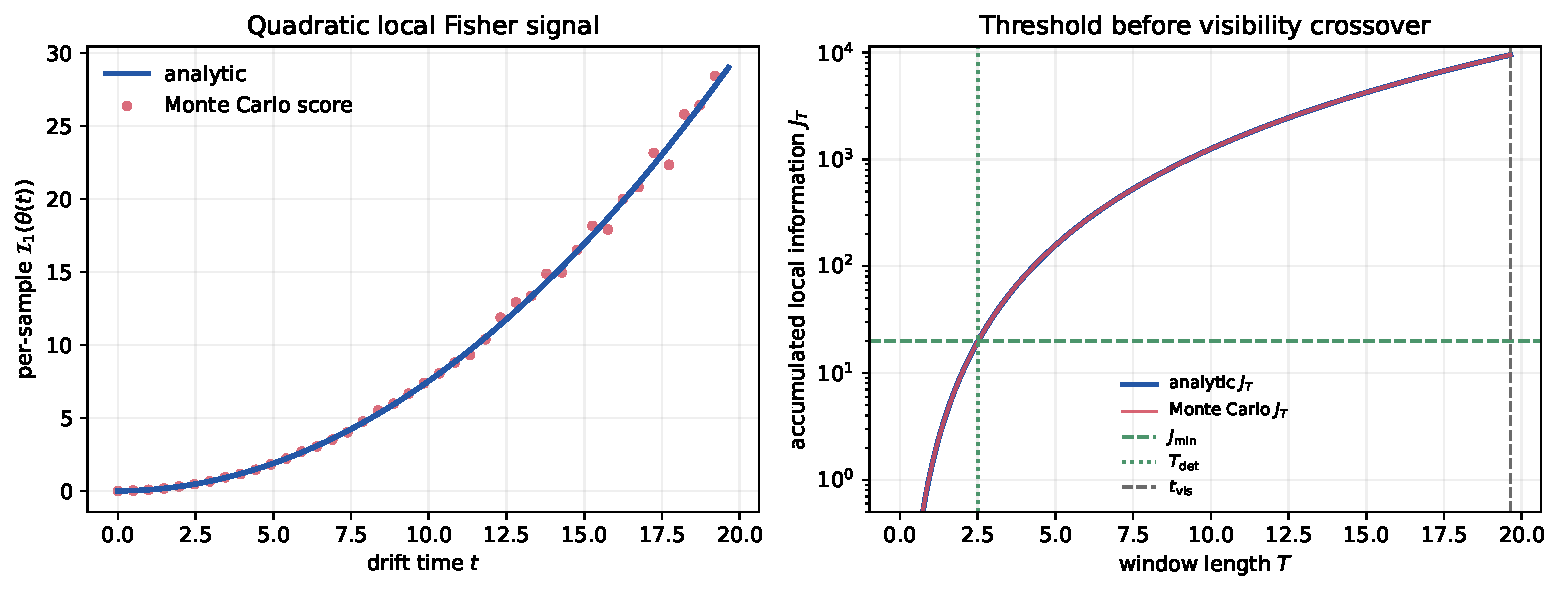
\includegraphics[width=\textwidth]{fig_fisher_residual.pdf}
\caption{\textbf{Direct score-based Fisher test.}
\textbf{Left:} analytic per-sample Fisher information and Monte Carlo
score-squared estimate, both quadratic in drift time.
\textbf{Right:} analytic and empirical accumulated local information;
the $J_{\min}=20$ crossing precedes the independently defined visibility
crossover for this parameter set.}
\label{III-fig:fisher_residual}
\end{figure}

% ------------------------------------------------------------
\subsection{Heuristic Calibration-Control Model}
\label{III-subsec:demo_model}

\paragraph{Environment.}
A $d$-dimensional linear prediction task:
$y(t) = \mathbf{w}(t)^\top \mathbf{x}(t)
+ \sigma\,\epsilon(t)$,
$\mathbf{x}(t) \sim \mathcal{N}(\mathbf{0}, \mathbf{I}_d)$,
$\epsilon \sim \mathcal{N}(0,1)$.
The weight vector $\mathbf{w}(t) \in \mathbb{S}^{d-1}$
drifts by receiving random perturbations on
\emph{background} dimensions only (indices $k,\ldots,d{-}1$),
then renormalising.  Signal therefore migrates progressively
from the ego's foreground to its blind sector.

\paragraph{Agents.}
\begin{itemize}
\item \textbf{Fixed ego} (Paper~II analogue):
  learns a linear model on a \emph{fixed} foreground
  subspace of dimension~$k$ via stochastic gradient descent
  (SGD, rate~$\eta$, decay~$\lambda$).
  Embodies the ``frozen gauge'' of Paper~II.
\item \textbf{Calibrated loop} (Paper~III analogue):
  identical ego plus a staleness sentinel and recalibration
  mechanism.
  The sentinel tracks $g_i = \mathrm{EMA}(|e\,x_i|)$ for
  each dimension~$i$ (an absolute-gradient proxy),
  computes the fraction of top-$k$ gradient dimensions
  \emph{not} in the current foreground as a frame-staleness
  index $m \in [0,1]$, and triggers
  recalibration when
  $\mathrm{EMA}(m) > \theta$.
  After recalibration, a settling period
  of~$\tau$ steps elapses before the sentinel resumes
  monitoring.
\end{itemize}

\paragraph{Parameters.}
\begin{center}
\small
\begin{tabular}{@{}lcl@{}}
\toprule
\textbf{Quantity} & \textbf{Value} & \textbf{Role} \\
\midrule
$d$ & 20 & full ambient dimension \\
$k$ & 5  & ego foreground dimension ($k/d = 0.25$) \\
$\sigma$ & 0.1 & observation noise std \\
$\eta$ & 0.01 & SGD learning rate \\
$\lambda$ & 0.998 & SGD weight decay \\
$\theta$ & 0.25 & staleness threshold \\
$\Lambda_{\mathrm{demo}}$ & variable & simulator drift amplitude per step \\
$\tau$ & variable & settling period (cooldown) \\
\bottomrule
\end{tabular}
\end{center}

\paragraph{Oracle metrics.}
Neither agent has access to $\mathbf{w}(t)$.
We evaluate performance externally using the \emph{oracle
full-space error}:
\begin{equation}
\label{III-eq:oracle_error}
\mathcal{E}_{\mathrm{full}}
= \bigl\|\mathbf{w}_{\mathrm{ego}}
  - \mathbf{w}^*_{\mathrm{fg}}\bigr\|^2
+ \bigl\|\mathbf{w}^*_{\mathrm{bg}}\bigr\|^2,
\end{equation}
where $\mathbf{w}^*_{\mathrm{fg}}$ and
$\mathbf{w}^*_{\mathrm{bg}}$ denote the true weight vector
restricted to foreground and background coordinates
respectively, and $\mathbf{w}_{\mathrm{ego}}$ is the ego's
foreground-supported estimator lifted to the full space.
The first term captures foreground tracking error (accessible
to the ego); the second captures hidden-sector signal
(invisible).

% ------------------------------------------------------------
\subsection{Results}
\label{III-subsec:demo_results}

\paragraph{Result 1: Delusion-correction separation
(Figure~\ref{III-fig:demo_trap}).}
At simulator drift amplitude $\Lambda_{\mathrm{demo}} = 0.02$,
settling period $\tau = 200$,
and $T = 5\,000$ steps, three phenomena are visible:

\begin{enumerate}
\item[(a)]
\emph{Delusion trap.}
The ego's foreground tracking error converges
to near zero, while the true full-space error rises
toward $\sim\!1$ and stabilises.
The growing gap between the two is the hidden sector in this supplied
linear model.  It does not prove a no-go theorem for all first-order
controllers.

\item[(b)]
\emph{Detectability.}
The staleness sentinel produces a clean sawtooth:
rising from zero after each recalibration, crossing the
threshold $\theta = 0.25$, and triggering frame reset
(25~events over $T = 5\,000$).
This demonstrates that the chosen overlap proxy can trigger a useful
reset.  The sentinel is not Fisher information; the direct Fisher test
is reported in Section~\ref{III-subsec:fisher_demo}.

\item[(c)]
\emph{Net benefit.}
The calibrated loop achieves
$\mathcal{E}_{\mathrm{full}} \approx 0.74$
versus the fixed ego's $\approx 1.02$:
a $27\%$ reduction in true prediction error.
\end{enumerate}

\begin{figure}[t]
\centering
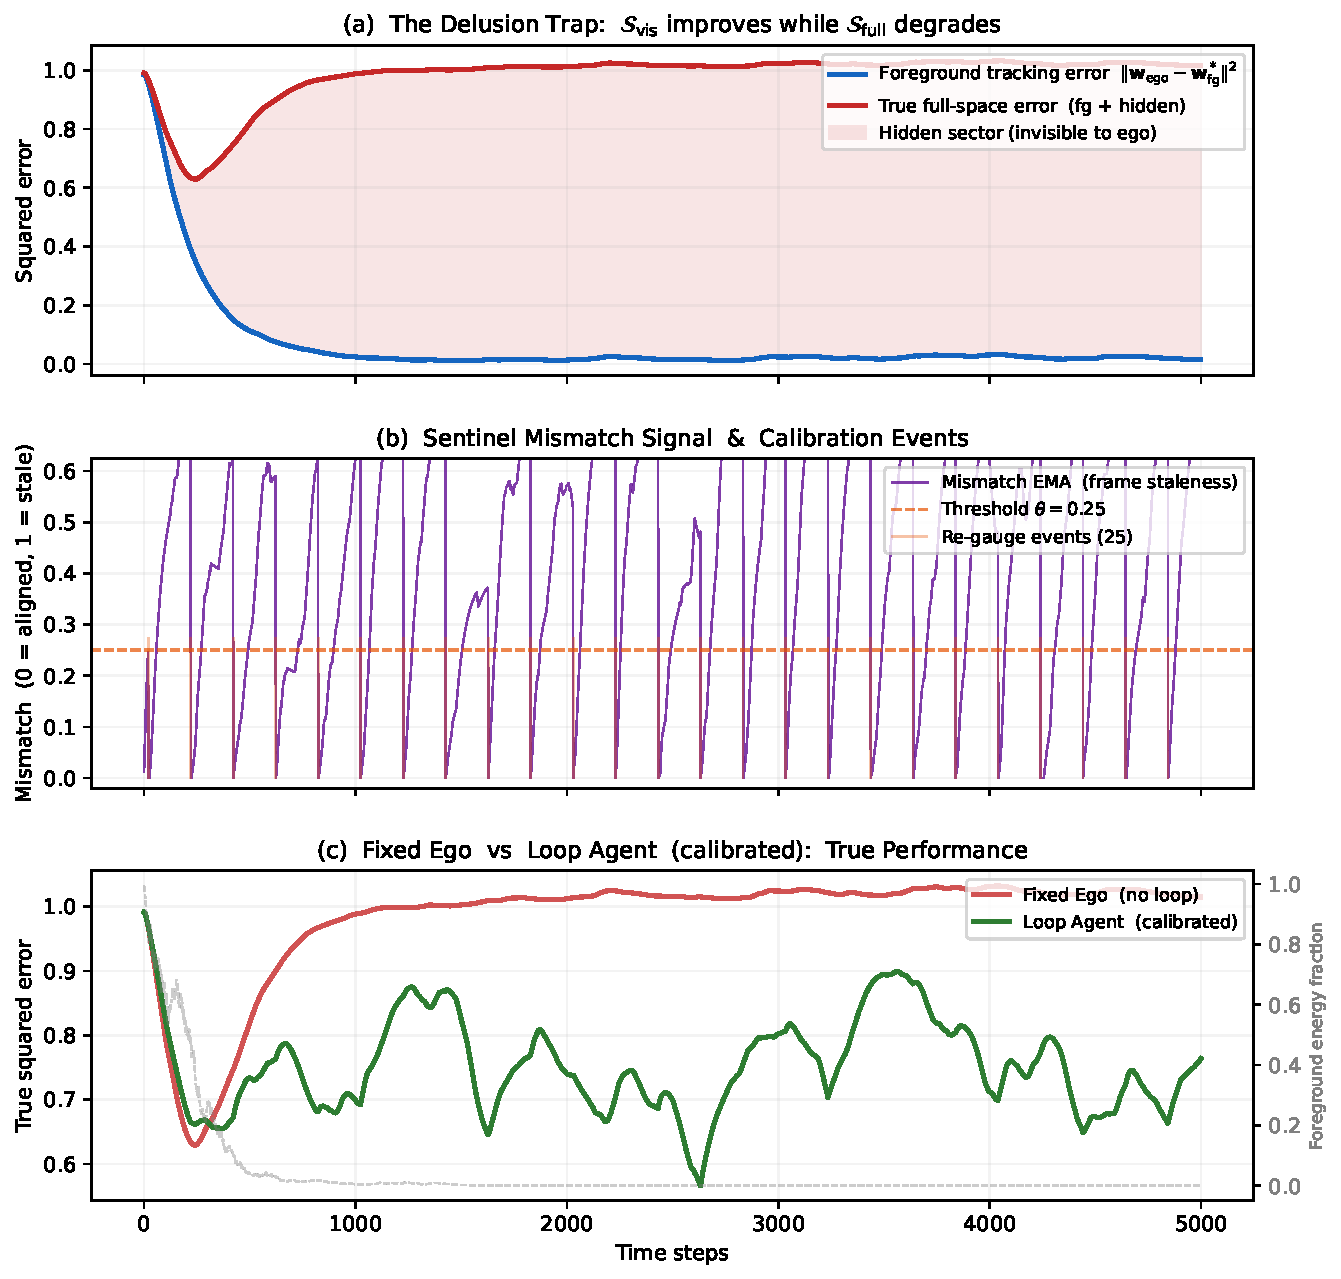
\includegraphics[width=\textwidth]{fig_delusion_trap.pdf}
\caption{%
\textbf{Delusion trap and calibration loop.}
$d = 20$, $k = 5$, $\Lambda_{\mathrm{demo}} = 0.02$,
$\tau = 200$,
$T = 5\,000$.
\textbf{(a)}~Foreground tracking error (blue) decreases
toward zero while true full-space error (red) increases;
the shaded region is the hidden sector, invisible to the ego.
\textbf{(b)}~Frame-staleness sentinel (purple) rises
monotonically between recalibration events (orange),
producing a sawtooth with 25 threshold crossings.
\textbf{(c)}~The calibrated loop (green) maintains
lower true error than the fixed ego (red);
the grey dashed line shows the foreground energy fraction
decaying as signal migrates to the background.}
\label{III-fig:demo_trap}
\end{figure}

\paragraph{Result 2: Phase structure and optimal
calibration budget
(Figures~\ref{III-fig:demo_phase}--\ref{III-fig:demo_alpha}).}
We scan 16 simulator drift amplitudes
$\Lambda_{\mathrm{demo}} \in [0.005, 0.08]$ and
16 settling periods $\tau \in [15, 800]$
(logarithmically spaced), running both agents for
$T = 4\,000$ steps across 6 random seeds per grid point.

Figure~\ref{III-fig:demo_phase}(a) shows the performance
gain $\Delta = \mathcal{E}_{\mathrm{ego}}
- \mathcal{E}_{\mathrm{loop}}$:
the loop improves over the ego (green) across most of
the parameter space, with a boundary at $\Delta = 0$
(dashed) below which recalibration is counterproductive
(very low drift, where the overhead of re-learning
exceeds the benefit of tracking).
The solid curve traces the \emph{optimal settling period}
$\tau_{\mathrm{opt}}(\Lambda_{\mathrm{demo}})$---the recalibration
period minimising $\mathcal{E}_{\mathrm{loop}}$---which
decreases monotonically from $\sim\!370$ steps at
$\Lambda_{\mathrm{demo}} = 0.005$ to $\sim\!100$ at
$\Lambda_{\mathrm{demo}} = 0.08$.
Figure~\ref{III-fig:demo_phase}(b) shows that calibration
frequency increases smoothly with drift and with shorter
settling period, exhibiting the cost--performance
trade-off of this supplied controller and cost proxy.  It does not test
Proposition~\ref{III-prop:loop_cost_impl}.

Extracting $\tau_{\mathrm{opt}}(\Lambda_{\mathrm{demo}})$ yields the
\emph{optimal calibration frequency}
$\alpha_{\mathrm{opt}}(\Lambda_{\mathrm{demo}})
= 1/\tau_{\mathrm{opt}}$
(Figure~\ref{III-fig:demo_alpha}).
The curve is smooth and monotonically increasing:
faster drift demands tighter calibration.
It saturates at high $\Lambda_{\mathrm{demo}}$ near
$\alpha_{\mathrm{opt}} \approx 0.01$ per step
($\tau_{\mathrm{opt}} \approx 100$), of the same
order as the learner's settling time.
This is consistent with the intuition that drift
estimation requires a minimum observation window;
the self-referential Cram\'{e}r--Rao bound
(Theorem~\ref{III-thm:SRCR}) provides the analytic
counterpart of this computational floor.

\begin{figure}[t]
\centering
\includegraphics[width=\textwidth]%
  {fig_phase_with_boundary.pdf}
\caption{%
\textbf{Phase structure and calibration cost.}
$16 \times 16$ grid, $T = 4\,000$, 6 seeds per point.
\textbf{(a)}~Performance gain $\Delta$; green = loop
improves on ego, red = counterproductive.
Solid curve: $\tau_{\mathrm{opt}}(\Lambda_{\mathrm{demo}})$.
Dashed: $\Delta = 0$ boundary.
\textbf{(b)}~Calibration frequency (thermodynamic cost
proxy: recalibration events per step, proportional to
energy expenditure under a fixed per-recalibration cost
model); $\tau_{\mathrm{opt}}$ overlaid.}
\label{III-fig:demo_phase}
\end{figure}

\begin{figure}[t]
\centering
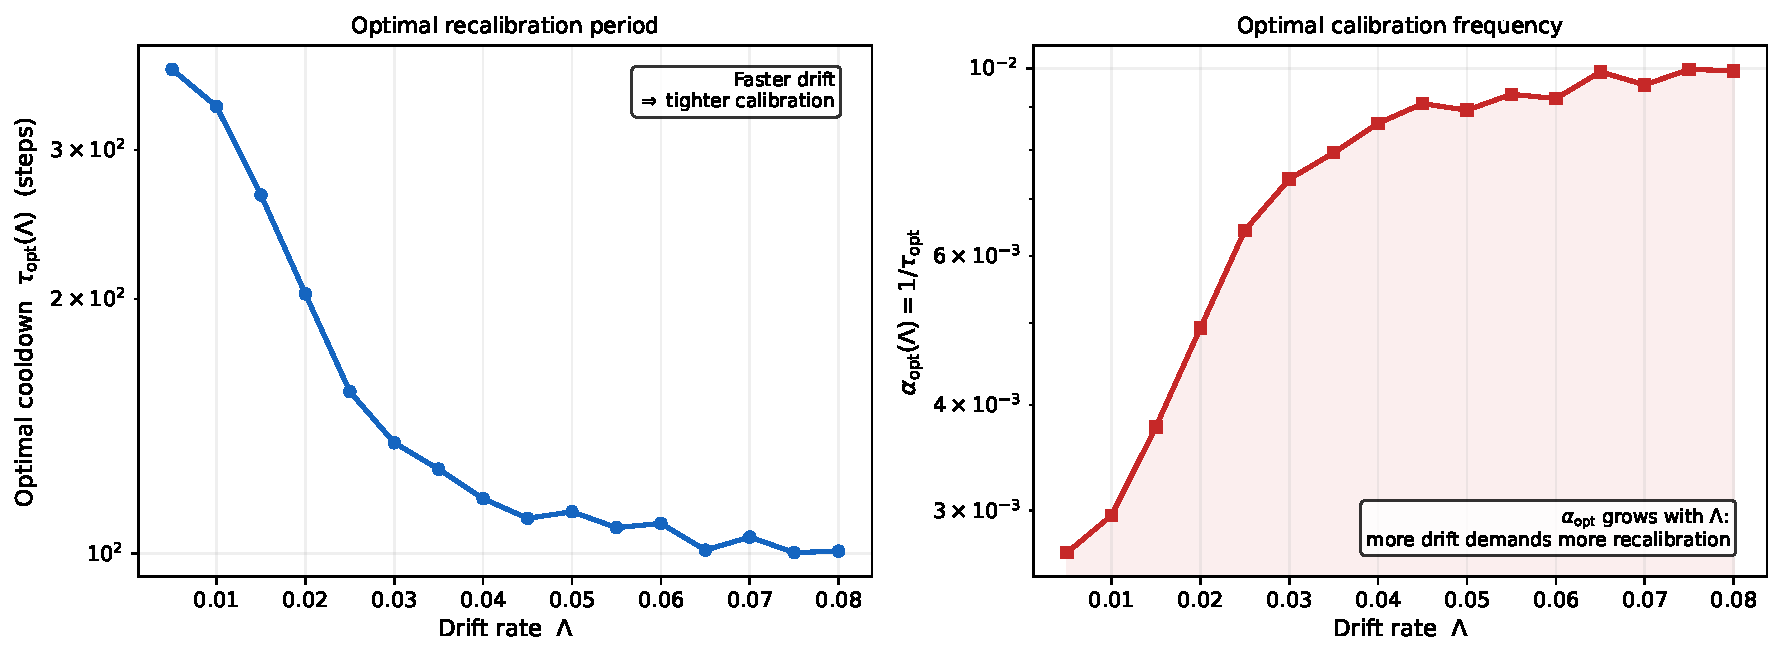
\includegraphics[width=\textwidth]{fig_alpha_opt.pdf}
\caption{%
\textbf{Optimal calibration frequency.}
\textbf{Left:}
$\tau_{\mathrm{opt}}(\Lambda_{\mathrm{demo}})$ decreases monotonically
with drift rate.
\textbf{Right:}
$\alpha_{\mathrm{opt}}(\Lambda_{\mathrm{demo}})
= 1/\tau_{\mathrm{opt}}$
increases with drift rate and saturates at the learner's
settling timescale ($\sim\!100$ steps), consistent with
an observation-window floor.}
\label{III-fig:demo_alpha}
\end{figure}

% ------------------------------------------------------------
\subsection{Scope of This Demonstration}
\label{III-subsec:demo_scope}

This demonstration \textbf{does} show:
\begin{enumerate}
\item The explicit Gaussian residual model has a directly measured
  score-squared Fisher signal with the quadratic and cubic scalings in
  Proposition~\ref{III-prop:gaussian_fisher}.
\item For the declared Gaussian parameters, the Fisher threshold is
  crossed before the linear visibility crossover.
\item A separate, non-Fisher frame-staleness proxy has clean threshold
  dynamics and triggers effective recalibration in the supplied linear
  controller.
\item An optimal calibration frequency
  $\alpha_{\mathrm{opt}}(\Lambda_{\mathrm{demo}})$ exists, increases
  monotonically with drift rate, and saturates at the
  learner's settling timescale in the scanned grid.
\end{enumerate}

\noindent
In summary, the direct experiment validates the declared Fisher
likelihood, while the controller experiment establishes a model-specific
proxy trade-off.  Neither is universal across architectures or
environment classes.

\medskip
This demonstration does \textbf{not} show:
\begin{enumerate}
\item That the specific functional form of
  $\alpha_{\mathrm{opt}}(\Lambda)$ matches the analytic
  Cram\'{e}r--Rao prediction in the
  large-$d$ limit.  The demonstration confirms the
  monotonic trend and saturation; deriving the exact
  scaling exponent from Theorem~\ref{III-thm:SRCR}
  remains open.
\item That the results generalise to all environment
  classes.  The model uses Gaussian features, linear
  regression, and isotropic background drift; extensions
  to non-linear, non-Gaussian, or structured-drift
  settings require further investigation.
\item That the calibration loop is optimal among all
  possible adaptive strategies.  It implements one
  specific realisation of the calibration-loop
  architecture.
\item That the gradient-overlap sentinel estimates Fisher information,
  or that recalibration-event frequency is a thermodynamic dissipation
  measurement.
\end{enumerate}

\paragraph{Reproducibility.}
\begin{sloppypar}
The controller simulation is in \texttt{tdome\_demo.py}.  The direct
Fisher experiment is in \texttt{fisher\_residual\_demo.py}, with raw
output in \texttt{fisher\_residual\_data.csv}.  Both require only NumPy
and Matplotlib and use fixed random seeds.
\end{sloppypar}

% ============================================================
\section{Discussion}
\label{III-sec:discussion}

% ------------------------------------------------------------
\subsection{Summary of Results}
\label{III-subsec:summary}

\begin{center}
\small
\setlength{\tabcolsep}{4pt}%
\begin{tabular}{@{}lP{6cm}c@{}}
\toprule
\textbf{Result} & \textbf{Statement} & \textbf{Sec.} \\
\midrule
Even-likelihood non-identifiability
  & The Gaussian residual record cannot identify mismatch sign
  & \ref{III-subsec:first_order} \\[3pt]
Drift Detectability
  & Per-sample FI is quadratic and accumulated local FI is cubic in the
    Gaussian linear-drift model
  & \ref{III-subsec:self_ref_fisher} \\[3pt]
Self-Referential CR Bound
  & Drift estimation bounded by
    $1/(n_{\mathrm{eff}}\,\mathbb E_\pi[\mathcal I_1]
    + \mathcal{I}_{\mathrm{ego}})$ under regular prior/likelihood data
  & \ref{III-subsec:SRCR} \\[3pt]
Loop Tracking Bound
  & Lyapunov $V$ with tracking neighbourhood
    $V_\infty = \|\dot{\sigma}^*\|^2/(\eta m_L)^2$ under local
    geodesic strong convexity
  & \ref{III-subsec:lyapunov} \\[3pt]
Four-Part Structure
  & Four supplied layers define the running model architecture
  & \ref{III-subsec:four_part} \\[3pt]
Loop Cost
  & $\dot{W}_{\mathrm{loop}} \geq k_BT\,\ln 2\,(R_s+R_c)
    + \mathcal{L}^2/\tau_{\mathrm{recalib}}^2$
    for a separable reset-based implementation
  & \ref{III-subsec:cost_theorem} \\[3pt]
Persistence Budget
  & Universal inherited budget withdrawn
  & \ref{III-subsec:persistence} \\[3pt]
Numerical Demonstration
  & Direct Fisher test plus a separate heuristic-controller scan
  & \ref{III-sec:numerical} \\
\bottomrule
\end{tabular}
\end{center}

% ------------------------------------------------------------
\subsection{Conditional Interface Sequence}
\label{III-subsec:logic_chain}

Papers~I--III provide a conditional interface sequence:

\begin{center}
\small
\setlength{\tabcolsep}{3pt}%
\begin{tabular}{@{}lP{3.2cm}P{3.8cm}l@{}}
\toprule
\textbf{Paper} & \textbf{Crisis} & \textbf{Resolution}
  & \textbf{What is born} \\
\midrule
Paper~I
  & Restricted autonomous baseline
  & Correlation-aware accounting
  & \textbf{Conditional resource model} \\[3pt]
Paper~II
  & Raw archive exceeds a declared budget
  & Supplied coordinate projection
  & \textbf{Frame model} \\[3pt]
Paper~III
  & Linear visibility loss in a fixed frame
  & Likelihood-based detection; conditional tracking
  & \textbf{Calibration model} \\
\bottomrule
\end{tabular}
\end{center}

The arrows are motivation or model interfaces.  The tracking theorem is
local and conditional, the universal persistence budget is withdrawn,
and no termination or completeness result follows.

% ------------------------------------------------------------
\subsection{What This Paper Does and Does Not Show}
\label{III-subsec:claims}

This paper \textbf{does} show:
\begin{enumerate}
\item The even Gaussian residual likelihood cannot identify mismatch
  sign, while its score has the explicit Fisher scalings in
  Proposition~\ref{III-prop:gaussian_fisher}.
\item Detection precedes visibility loss exactly when the threshold
  condition in Corollary~\ref{III-cor:detection_window} holds.
\item Drift estimation precision is bounded by the
  Self-Referential Cram\'{e}r--Rao bound
  (Theorem~\ref{III-thm:SRCR}).
\item The calibration loop tracks the optimal frame
  within a bounded neighbourhood under a Lyapunov
  tracking bound
  (Theorem~\ref{III-thm:loop_stability}).
\item A separable reset-based hardware model obeys the conditional cost
  bound in Proposition~\ref{III-prop:loop_cost_impl}.
\end{enumerate}

\medskip
This paper does \textbf{not} show:
\begin{enumerate}
\item That self-referential calibration implies or requires
  phenomenal consciousness, subjective experience, or
  qualia. ``Reflexivity'' as used here denotes
  second-order control, nothing more.
\item That the Lyapunov function $V$ is a measure of
  ``awareness.'' It is a control-theoretic stability
  condition, not a consciousness metric.
\item That the four-part template is necessary, sufficient, or a
  complete characterisation of agency.
\item That Fisher information requires the agent to
  ``know'' it is computing Fisher information.
  The computation can be implemented implicitly by any
  physical system whose dynamics approximate the natural
  gradient.
\item That the calibration loop eliminates the ego's bias.
  It tracks and compensates for drift in the bias;
  the four bias terms of Paper~II persist.
\item That sensing or computing is intrinsically dissipative.  The
  Landauer terms require irreversible register reset.
\item That this framework applies to all possible systems.
  It applies to systems satisfying~(C1)--(C5).
\item That the structural parallel with philosophical
  concepts of self-awareness constitutes a philosophical
  or metaphysical claim.
\item That the Clifford algebra is the only possible
  algebraic setting. Other control algebras may yield
  analogous results with different quantitative bounds.
\end{enumerate}

\medskip
We have established a checkable Gaussian Fisher signal, a regular
Bayesian estimation bound, and a local tracking result.  Their use in a
physical agent remains conditional on the declared observation,
optimization, and hardware models.

% ============================================================
% REFERENCES
% ============================================================


\backmatter

% ============================================================================
% UNIFIED BIBLIOGRAPHY
% ============================================================================
\begin{thebibliography}{99}

\bibitem{Amari1985}
S.-i.~Amari,
\emph{Differential-Geometrical Methods in Statistics},
Lecture Notes in Statistics \textbf{28}, Springer (1985).

\bibitem{Amari1998}
S.-i.~Amari,
\emph{Natural gradient works efficiently in learning},
Neural Computation \textbf{10}, 251 (1998).

\bibitem{AmariNagaoka2000}
S.-i.~Amari and H.~Nagaoka,
\emph{Methods of Information Geometry},
Translations of Mathematical Monographs \textbf{191},
AMS (2000).

\bibitem{Ashby1956}
W.~R.~Ashby,
\emph{An Introduction to Cybernetics},
Chapman \& Hall (1956).

\bibitem{AstromWittenmark1995}
K.~J.~\AA{}str\"{o}m and B.~Wittenmark,
\emph{Adaptive Control},
2nd ed., Addison-Wesley (1995).

\bibitem{BaratoSeifert2015}
A.~C.~Barato and U.~Seifert,
\emph{Thermodynamic uncertainty relation for biomolecular
processes},
Phys.\ Rev.\ Lett.\ \textbf{114}, 158101 (2015).

\bibitem{Bennett1982}
C.~H.~Bennett,
\emph{The thermodynamics of computation---a review},
Int.\ J.\ Theor.\ Phys.\ \textbf{21}, 905 (1982).

\bibitem{BialekNemenmanTishby2001}
W.~Bialek, I.~Nemenman, and N.~Tishby,
\emph{Predictability, complexity, and learning},
Neural Computation \textbf{13}, 2409 (2001).

\bibitem{BreuerLainePiilo2009}
H.-P.~Breuer, E.-M.~Laine, and J.~Piilo,
\emph{Measure for the Degree of Non-Markovian Behavior of Quantum Processes in Open Systems},
Phys.\ Rev.\ Lett.\ \textbf{103}, 210401 (2009).

\bibitem{BreuerPetruccione2002}
H.-P.~Breuer and F.~Petruccione,
\emph{The Theory of Open Quantum Systems},
Oxford University Press (2002).

\bibitem{Cencov1982}
N.~N.~\v{C}encov,
\emph{Statistical Decision Rules and Optimal Inference},
Translations of Mathematical Monographs \textbf{53},
AMS (1982).

\bibitem{CoverThomas2006}
T.~M.~Cover and J.~A.~Thomas,
\emph{Elements of Information Theory},
2nd ed., Wiley (2006).

\bibitem{Crooks2007}
G.~E.~Crooks,
\emph{Measuring thermodynamic length},
Phys.\ Rev.\ Lett.\ \textbf{99}, 100602 (2007).

\bibitem{CrutchfieldYoung1989}
J.~P.~Crutchfield and K.~Young,
\emph{Inferring statistical complexity},
Phys.\ Rev.\ Lett.\ \textbf{63}, 105 (1989).

\bibitem{EspositoLindenbergVandenBroeck2010}
M.~Esposito, K.~Lindenberg, and C.~Van~den~Broeck,
\emph{Entropy production as correlation between system and reservoir},
New J.\ Phys.\ \textbf{12}, 013013 (2010).

\bibitem{GKS1976}
V.~Gorini, A.~Kossakowski, and E.~C.~G.~Sudarshan,
\emph{Completely positive dynamical semigroups of $N$-level systems},
J.\ Math.\ Phys.\ \textbf{17}, 821 (1976).

\bibitem{GovernTenWolde2014}
W.~P.~Govern and P.~R.~ten~Wolde,
\emph{Optimal resource allocation in cellular sensing systems},
Proc.\ Natl.\ Acad.\ Sci.\ USA \textbf{111}, 17486 (2014).

\bibitem{Ito2018}
S.~Ito,
\emph{Stochastic thermodynamic interpretation of
information geometry},
Phys.\ Rev.\ Lett.\ \textbf{121}, 030605 (2018).

\bibitem{JohnsonLindenstrauss1984}
W.~B.~Johnson and J.~Lindenstrauss,
\emph{Extensions of Lipschitz mappings into a Hilbert space},
Contemp.\ Math.\ \textbf{26}, 189 (1984).

\bibitem{Landauer1961}
R.~Landauer,
\emph{Irreversibility and heat generation in the computing process},
IBM J.\ Res.\ Dev.\ \textbf{5}, 183 (1961).

\bibitem{Lindblad1976}
G.~Lindblad,
\emph{On the generators of quantum dynamical semigroups},
Commun.\ Math.\ Phys.\ \textbf{48}, 119 (1976).

\bibitem{MehtaSchwab2012}
P.~Mehta and D.~J.~Schwab,
\emph{Energetic costs of cellular computation},
Proc.\ Natl.\ Acad.\ Sci.\ USA \textbf{109}, 17978 (2012).

\bibitem{Nakajima1958}
S.~Nakajima,
\emph{On quantum theory of transport phenomena},
Prog.\ Theor.\ Phys.\ \textbf{20}, 948 (1958).

\bibitem{PooleOzairVanDenOord2019}
B.~Poole, S.~Ozair, A.~Van~Den~Oord, A.~Alemi, and G.~Tucker,
\emph{On variational bounds of mutual information},
Proc.\ ICML, PMLR \textbf{97}, 5171--5180 (2019).

\bibitem{Rao1945}
C.~R.~Rao,
\emph{Information and the accuracy attainable in the
estimation of statistical parameters},
Bull.\ Calcutta Math.\ Soc.\ \textbf{37}, 81 (1945).

\bibitem{RivasHuelgaPlenio2014}
\'{A}.~Rivas, S.~F.~Huelga, and M.~B.~Plenio,
\emph{Quantum non-Markovianity: characterization, quantification and detection},
Rep.\ Prog.\ Phys.\ \textbf{77}, 094001 (2014).

\bibitem{SagawaUeda2010}
T.~Sagawa and M.~Ueda,
\emph{Generalized Jarzynski Equality under Nonequilibrium Feedback Control},
Phys.\ Rev.\ Lett.\ \textbf{104}, 090602 (2010).

\bibitem{SagawaUeda2012}
T.~Sagawa and M.~Ueda,
\emph{Fluctuation Theorem with Information Exchange},
Phys.\ Rev.\ Lett.\ \textbf{109}, 180602 (2012).

\bibitem{Schrodinger1944}
E.~Schr\"odinger,
\emph{What is Life?},
Cambridge University Press (1944).

\bibitem{ShaliziCrutchfield2001}
C.~R.~Shalizi and J.~P.~Crutchfield,
\emph{Computational mechanics: Pattern and prediction, structure and simplicity},
J.\ Stat.\ Phys.\ \textbf{104}, 817 (2001).

\bibitem{Shannon1959}
C.~E.~Shannon,
\emph{Coding theorems for a discrete source with a
fidelity criterion},
IRE Nat.\ Conv.\ Rec., Part~4, pp.~142--163 (1959).

\bibitem{Simon1955}
H.~A.~Simon,
\emph{A behavioral model of rational choice},
Quarterly J.\ of Economics \textbf{69}, 99 (1955).

\bibitem{Sims2003}
C.~A.~Sims,
\emph{Implications of rational inattention},
J.\ Monetary Economics \textbf{50}, 665 (2003).

\bibitem{SivakCrooks2012}
D.~A.~Sivak and G.~E.~Crooks,
\emph{Thermodynamic metrics and optimal paths},
Phys.\ Rev.\ Lett.\ \textbf{108}, 190602 (2012).

\bibitem{Spohn1978}
H.~Spohn,
\emph{Entropy production for quantum dynamical semigroups},
J.\ Math.\ Phys.\ \textbf{19}, 1227 (1978).

\bibitem{Tishby2000}
N.~Tishby, F.~C.~Pereira, and W.~Bialek,
\emph{The information bottleneck method},
in Proc.\ 37th Allerton Conf.\ on Communication, Control,
and Computing (1999); arXiv:physics/0004057 (2000).

\bibitem{Zurek2009}
W.~H.~Zurek,
\emph{Quantum Darwinism},
Nature Physics \textbf{5}, 181 (2009).

\bibitem{Zwanzig1960}
R.~Zwanzig,
\emph{Ensemble method in the theory of irreversibility},
J.\ Chem.\ Phys.\ \textbf{33}, 1338 (1960).

\bibitem{vanTrees1968}
H.~L.~van Trees,
\emph{Detection, Estimation, and Modulation Theory},
Part~I, Wiley (1968).

\bibitem{vonFoerster2003}
H.~von Foerster,
\emph{Understanding Understanding: Essays on Cybernetics
and Cognition},
Springer (2003).

\bibitem{Liu2026HAFF_A}
S.~Liu, \emph{Emergent Geometry from Coarse-Grained Observable Algebras: The Holographic Alaya-Field Framework}, Zenodo (2026), DOI: 10.5281/zenodo.18361706.

\bibitem{Liu2026HAFF_B}
S.~Liu, \emph{Accessibility, Stability, and Emergent Geometry: Conceptual Clarifications on the Holographic Alaya-Field Framework}, Zenodo (2026), DOI: 10.5281/zenodo.18367060.

\bibitem{Liu2026HAFF_C}
S.~Liu, \emph{Causation, Agency, and Existence: Structural Constraints and Interpretive Bridges}, Zenodo (2026), DOI: 10.5281/zenodo.18374805.

\bibitem{Liu2026HAFF_F}
S.~Liu, \emph{Accessibility Propagation and Temporal Direction: A Conditional Structural Analysis}, Zenodo (2026), DOI: 10.5281/zenodo.18400425.

\bibitem{Liu2026HAFF_G}
S.~Liu, \emph{Structural Limits of Unification: Accessibility, Incompleteness, and a Programme-Level Final-Cut Diagnosis}, Zenodo (2026), DOI: 10.5281/zenodo.18402907.

\bibitem{Liu2026QRAIF_A}
S.~Liu, \emph{A Clifford-Encoding Model for Lorentzian Metrics in Entropic Gravity Frameworks}, Zenodo (2026), DOI: 10.5281/zenodo.18525876.

\bibitem{Liu2026QRAIF_B}
S.~Liu, \emph{Thermodynamic Stability Constraints on the Operator Algebra of Persistent Open Quantum Subsystems}, Zenodo (2026), DOI: 10.5281/zenodo.18525890.

\bibitem{Liu2026QRAIF_C}
S.~Liu, \emph{Conditional Image-Level Closure in the Q-RAIF Framework}, Zenodo (2026), DOI: 10.5281/zenodo.18528934.

\bibitem{Liu2026TDOME_I}
S.~Liu, \emph{Non-Markovian Memory and Temporal Accumulation: A Conditional Thermodynamic Analysis}, Zenodo (2026), DOI: 10.5281/zenodo.18574342.

\bibitem{Liu2026TDOME_II}
S.~Liu, \emph{Spontaneous Symmetry Breaking of Reference Frames as a Computational Cost Minimization Strategy}, Zenodo (2026), DOI: 10.5281/zenodo.18579703.

\end{thebibliography}

\end{document}
